
%========= File containing the main LaTex document ========%
%                                                          %
% Copyright (C) ISI - All Rights Reserved                  %
% Proprietary                                              %
% Written by Med Hossam <med.hossam@gmail.com>, April 2016 %
%                                                          %
% @author: HEDHILI Med Houssemeddine                       %
% @linkedin: http://tn.linkedin.com/in/medhossam           %
%==========================================================%

%\documentclass[pfe]{./tpl/isipfe}
\documentclass[]{./tpl/isipfe}
\graphicspath{{./img/}}

\usepackage{hyperref}
\usepackage{acronym}
\usepackage{subfig}

%=========== File containing some new commands ============%
%                                                          %
% Copyright (C) ISI - All Rights Reserved                  %
% Proprietary                                              %
% Written by Med Hossam <med.hossam@gmail.com>, April 2016 %
%                                                          %
% @author: HEDHILI Med Houssemeddine                       %
% @linkedin: http://tn.linkedin.com/in/medhossam           %
%==========================================================%

\newenvironment{changemargin}[2]{%
\begin{list}{}{%
\setlength{\leftmargin}{#1}%
\setlength{\rightmargin}{#2}%
}%
\item[]}
{\end{list}}

\makeatletter

%================= front cover variables =================%

\newcommand{\secondAuthor}[1]{\gdef\@secondAuthor{#1}}%
\newcommand{\@secondAuthor}{\@latex@warning@no@line{No \noexpand\secondAuthor given}}

\newcommand{\diplomaName}[1]{\gdef\@diplomaName{#1}}%
\newcommand{\@diplomaName}{\@latex@warning@no@line{No \noexpand\diplomaName given}}

\newcommand{\speciality}[1]{\gdef\@speciality{#1}}%
\newcommand{\@speciality}{\@latex@warning@no@line{No \noexpand\speciality given}}

\newcommand{\proFramerName}[1]{\gdef\@proFramerName{#1}}%
\newcommand{\@proFramerName}{\@latex@warning@no@line{No \noexpand\proFramerName given}}

\newcommand{\proFramerSpeciality}[1]{\gdef\@proFramerSpeciality{#1}}%
\newcommand{\@proFramerSpeciality}{\@latex@warning@no@line{No \noexpand\proFramerSpeciality given}}

\newcommand{\academicFramerName}[1]{\gdef\@academicFramerName{#1}}%
\newcommand{\@academicFramerName}{\@latex@warning@no@line{No \noexpand\academicFramerName given}}

\newcommand{\academicFramerSpeciality}[1]{\gdef\@academicFramerSpeciality{#1}}%
\newcommand{\@academicFramerSpeciality}{\@latex@warning@no@line{No \noexpand\academicFramerSpeciality given}}

\newcommand{\collegeYear}[1]{\gdef\@collegeYear{#1}}%
\newcommand{\@collegeYear}{\@latex@warning@no@line{No \noexpand\collegeYear given}}

\newcommand{\companyName}[1]{\gdef\@companyName{#1}}%
\newcommand{\@companyName}{\@latex@warning@no@line{No \noexpand\companyName given}}

%================== Signatures variables ==================%

\newcommand{\proSignSentence}[1]{\gdef\@proSignSentence{#1}}%
\newcommand{\@proSignSentence}{\@latex@warning@no@line{No \noexpand\proSignSentence given}}

\newcommand{\academicSignSentence}[1]{\gdef\@academicSignSentence{#1}}%
\newcommand{\@academicSignSentence}{\@latex@warning@no@line{No \noexpand\academicSignSentence given}}

%================== Backcover variables ==================%

\newcommand{\arabicAbstract}[1]{\gdef\@arabicAbstract{#1}}%
\newcommand{\@arabicAbstract}{\@latex@warning@no@line{No \noexpand\arabicAbstract given}}

\newcommand{\arabicAbstractKeywords}[1]{\gdef\@arabicAbstractKeywords{#1}}%
\newcommand{\@arabicAbstractKeywords}{\@latex@warning@no@line{No \noexpand\arabicAbstractKeywords given}}

\newcommand{\frenchAbstract}[1]{\gdef\@frenchAbstract{#1}}%
\newcommand{\@frenchAbstract}{\@latex@warning@no@line{No \noexpand\frenchAbstract given}}

\newcommand{\frenchAbstractKeywords}[1]{\gdef\@frenchAbstractKeywords{#1}}%
\newcommand{\@frenchAbstractKeywords}{\@latex@warning@no@line{No \noexpand\frenchAbstractKeywords given}}

\newcommand{\englishAbstract}[1]{\gdef\@englishAbstract{#1}}%
\newcommand{\@englishAbstract}{\@latex@warning@no@line{No \noexpand\englishAbstract given}}

\newcommand{\englishAbstractKeywords}[1]{\gdef\@englishAbstractKeywords{#1}}%
\newcommand{\@englishAbstractKeywords}{\@latex@warning@no@line{No \noexpand\englishAbstractKeywords given}}

\newcommand{\companyEmail}[1]{\gdef\@companyEmail{#1}}%
\newcommand{\@companyEmail}{\@latex@warning@no@line{No \noexpand\companyEmail given}}

\newcommand{\companyTel}[1]{\gdef\@companyTel{#1}}%
\newcommand{\@companyTel}{\@latex@warning@no@line{No \noexpand\companyTel given}}

\newcommand{\companyFax}[1]{\gdef\@companyFax{#1}}%
\newcommand{\@companyFax}{\@latex@warning@no@line{No \noexpand\companyFax given}}

\newcommand{\companyAddressFR}[1]{\gdef\@companyAddressFR{#1}}%
\newcommand{\@companyAddressFR}{\@latex@warning@no@line{No \noexpand\companyAddressFR given}}

\newcommand{\companyAddressAR}[1]{\gdef\@companyAddressAR{#1}}%
\newcommand{\@companyAddressAR}{\@latex@warning@no@line{No \noexpand\companyAddressAR given}}

%============= cmd for inserting blank page =============%
\newcommand\blankpage{%
    \null
    \thispagestyle{empty}%
    \addtocounter{page}{-1}%
    \newpage}

%================ document main language ================%
%\selectlanguage{english}
\selectlanguage{french}

%================== required packages ===================%

\usepackage{tcolorbox}
\usepackage{afterpage}
\usepackage{array,longtable,multirow}% http://ctan.org/pkg/{array,longtable,multirow}
\usepackage{pifont}

\usepackage{pdflscape}
\usepackage{rotating}
\usepackage{wrapfig}
\setlength{\parskip}{0pt} % Espacement vertical entre les paragraphes (par exemple, 12pt)
\setlength{\parindent}{0pt}
% @author: Stoufa
% the command `\makeindex` is mandatory to create the index file main.idx
% https://tex.stackexchange.com/questions/9913/input-index-file-not-found
\makeindex
\begin{document}
    
%=== File containing Global Configuration of the report ===%
%                                                          %
% Copyright (C) ISI - All Rights Reserved                  %
% Proprietary                                              %
% Written by Med Hossam <med.hossam@gmail.com>, April 2016 %
%                                                          %
% @author: HEDHILI Med Houssemeddine                       %
% @linkedin: http://tn.linkedin.com/in/medhossam           %
%==========================================================%

%=========== You MUST type your information here ==========%
% global_config.tex file is designed to configure your     %
% cover pages (main, back and black covers)                %
%==========================================================%

%============= Config new columns type ==============%
\newcolumntype{L}{>{\raggedright\arraybackslash}}
\newcolumntype{R}{>{\raggedleft\arraybackslash}}
\newcolumntype{C}{>{\centering\arraybackslash}}
%==================================================%

%========= Config the cover section ==========%

\title{Conception et développement d'une platforme analytique pour les méta-données de Snowflake }

\author{Ons CHAHED}
%%% if necessary
% Set isBinomal to true and type second author name
%\setboolean{isBinomal}{true}
%\secondAuthor{Prénom NOM}

\diplomaName{Diplôme National d'ingénieur}
\speciality{Ingénierie du Développement du Logiciel( IDL)}

%\speciality{Génie des Télécommunications et Réseaux}
%\speciality{Génie Informatique des Systèmes Industriels}

%% Encadrant professionnel
\proFramerName{Monsieur Nassim JALLOUD}
\proFramerSpeciality {Directeur adjoint du département Intégration et développement }

%% Encadrant académique
\academicFramerName{Monsieur Sahbi BAHROUN}
\academicFramerSpeciality{Maître Assistant}

%% Entreprise d'accueil
\companyName{Avaxia Group}

%% Année universitaire
\collegeYear{2023 - 2024}

%%%%%% Signatures section %%%%%%

% You can simply remove theses sentences by typing an empty string
% \proSignSentence{}

\proSignSentence{J'autorise l'étudiant à faire le dépôt de son rapport de stage de fin d'études en vue de l'obtention du diplôme national d'ingénieur.}

\academicSignSentence{J'autorise l'étudiant à faire le dépôt de son rapport de stage de fin d'études en vue de l'obtention du diplôme national d'ingénieur.}

%%% AR
\arabicAbstract{ هذا العمل هو جزء من مشروع ختم الدروس الهندسية في المعهد العالي للإعلامية للسنة الدراسية 2023-2024. لقد أجرينا تدريباً مع شركة \textLR{Avaxia Group} في نهاية الدراسة بهدف تصميم وتنفيذ منصة تحليلية لتصور البيانات الوصفية لـ Snowflake. يستخدم هذا الحل بنية الخدمات المصغرة لتوفير المرونة والنمطية وقابلية التوسع, دمج خدمات التحليل والمراقبة في الوقت الفعلي لتحسين الأداء وإدارة البيانات.}
\arabicAbstractKeywords{تحليل البيانات, \textLR{FastAPI}, \textLR{PostgreSQL}, \textLR{Snowflake}, \textLR{ReactJS}, \textLR{Kanban}, الخدمات المصغرة }

%% To use latin characters inside the arabic text
% just put them inside the command \textLR{}
%%%%

%%% FR
\frenchAbstract{Ce travail s'inscrit dans le cadre de l'accomplissement de notre Projet de Fin d'Études d'ingénieur à l'Institut Supérieur
d'Informatique pour l'année universitaire 2023-2024. Nous avons effectué ce stage au sein du Avaxia Group, qui ayant comme objectif de concevoir et implémenter une plateforme analytique pour la 
visualisation des métadonnées de Snowflake. Cette solution utilise une architecture microservices pour offrir flexibilité, modularité et évolutivité, 
intégrant des services d'analyse et de monitoring en temps réel pour optimiser les performances et la gestion des données.}

\frenchAbstractKeywords{\textbf{Analyse de données},\textbf{FastAPI},\textbf{PostgreSQL},\textbf{Snowflake},\textbf{ReactJS}, \textbf{Kanban}, \textbf{Microservices}.}

%%% EN
\englishAbstract{This work is part of the completion of our Final Engineering Project at the higher institute of computer science for the academic year 2023-2024.
 We carried out an end-of-study internship with the Avaxia Group with the aim of designing and implementing an 
 analytical platform for the visualisation of Snowflake metadata. This solution uses a microservices architecture 
 to offer flexibility, modularity and scalability, 
integrating real-time analysis and monitoring services to optimise performance and data management.}

\englishAbstractKeywords{\textbf{Data analysis}, \textbf{FastAPI},\textbf{PostgreSQL},\textbf{Snowflake},\textbf{ReactJS}, \textbf{Kanban}, \textbf{Microservices}.}

%% if you want to get rid of the company address just set the boolean variable to false
% PS : it's optional
\setboolean{wantToTypeCompanyAddress}{true}

\companyEmail{contact@avaxia-group.com}
\companyTel{71 904 013}
\companyAddressAR{منبلازير - تونس}
\companyAddressFR{A01, Mont-plaisir, AV Khaireddine PACHA CP 1073}
    
    \frontmatter
        
%===== File containing the main cover of the document =====%
%                                                          %
% Copyright (C) ISI - All Rights Reserved                  %
% Proprietary                                              %
% Written by Med Hossam <med.hossam@gmail.com>, April 2016 %
%                                                          %
% @author: HEDHILI Med Houssemeddine                       %
% @linkedin: http://tn.linkedin.com/in/medhossam           %
%==========================================================%

%== It's advised to not modify the content of this file ===%
% To set your information, go to global_config.tex file    %
%==========================================================%

\thispagestyle{cover}%
\newgeometry{bottom=25mm,left=20mm,top=15mm,right=20mm}
\hspace{-47pt}
\begin{minipage}[l]{0.2\columnwidth}
\vspace{6mm}

\includegraphics[width=1.1\columnwidth]{LogoISI}\\
\end{minipage}
\hfill
\begin{minipage}[l]{0.6\columnwidth}
\centering
\footnotesize
\textbf{{République Tunisienne}}\\
\vspace{1.5mm}
\textbf{{Ministère de l'Enseignement Supérieur\\
et de la Recherche Scientifique}}\\
\vspace{1.5mm}
\textbf{{Université de Tunis El Manar}}\\
\vspace{1.5mm}
\textbf{{Institut Supérieur d'Informatique d’El Manar}}
\end{minipage}
\hfill
\begin{minipage}[l]{0.02\columnwidth}
\end{minipage}
\hfill
\begin{minipage}[l]{0.18\columnwidth}
\vspace{6mm}

\includegraphics[width=0.9\columnwidth]{Logo_UTM}\\
\end{minipage}
\vskip1.5cm

\begin{center}
{\LARGE{\textbf{\textsc{rapport de projet de fin d'année}}}}\\
\vskip0.5cm
\large

{\textbf{Présenté en vue de la validation du}}\\
\vskip2mm
{\textbf{\@diplomaName}}\\
{\textbf{Spécialité : \@speciality}}\\
{}
\end{center}

\begin{center}
\textrm{Par}\\
\vskip0.3cm
{\ifthenelse{\boolean{isBinomal}}
    {% IF TRUE
        \begin{center}
            \large\textbf{\@author}~~~~~ et ~~~~~
            \large\textbf{\@secondAuthor}
        \end{center}
    }
    {\Large\textbf{\@author}}% FALSE
}
\vskip12mm

\definecolor{isiBlue}{RGB}{31, 78, 121}

\begin{changemargin}{-9mm}{0cm}
\begin{minipage}[l]{1.1\columnwidth}
\begin{tcolorbox}[colframe=isiBlue,colback=white,boxrule=0pt,toprule=3pt,bottomrule=3pt,arc=0pt,top=0mm,right=0mm,left=0mm,bottom=0mm,boxsep=0.5mm]{
    \begin{tcolorbox}[colframe=isiBlue,colback=white, boxrule=0pt,toprule=1pt,bottomrule=1pt,arc=0pt,enlarge bottom by=-0.9mm, auto outer arc]
        \centering
        {\huge\textbf{\@title}}
    \end{tcolorbox}
}
\end{tcolorbox}
\end{minipage}
\end{changemargin}

\end{center}
\vskip8mm%

\begin{center}
\large
\begin{minipage}[c]{0.28\columnwidth}
Encadrant professionnel:\\
Encadrant académique:
\end{minipage}
\hfill
\begin{minipage}[c]{0.42\columnwidth}
\textbf{\@proFramerName}\\
\textbf{\@academicFramerName}
\end{minipage}
\hfill
\begin{minipage}[c]{0.26\columnwidth}
\@proFramerSpeciality\\
\@academicFramerSpeciality
\end{minipage}
\end{center}
\vskip16mm

\begin{center}
\large
Réalisé au sein de \@companyName\\
\vskip0.4cm
\begin{figure}[h]
\centering
{\color{isiBlue}{\fboxrule=2.5pt\fbox{
\includegraphics[width=0.3\columnwidth]{Logo_Entreprise}}}}
\end{figure}
\end{center}

\afterpage{\blankpage}
        
%===== File containing the black cover of the document ====%
%                                                          %
% Copyright (C) ISI - All Rights Reserved                  %
% Proprietary                                              %
% Written by Med Hossam <med.hossam@gmail.com>, April 2016 %
%                                                          %
% @author: HEDHILI Med Houssemeddine                       %
% @linkedin: http://tn.linkedin.com/in/medhossam           %
%==========================================================%

%== It's advised to not modify the content of this file ===%
% To set your information, go to global_config.tex file    %
%==========================================================%

\thispagestyle{cover}%
\begin{minipage}[l]{0.2\columnwidth}
\vspace{6mm}
\hspace{+25mm}


\includegraphics[width=1.1\columnwidth]{Logo_ISI_Black}\\
\end{minipage}
\hfill
\begin{minipage}[l]{0.6\columnwidth}
\centering
\footnotesize
\hspace{-5mm}
\textbf{{République Tunisienne}}\\
\vspace{1.5mm}
\hspace{-5mm}
\textbf{{Ministère de l'Enseignement Supérieur\\
et de la Recherche Scientifique}}\\
\hspace{-5mm}

\textbf{{Université de Tunis El Manar}}\\
\hspace{-5mm}

\textbf{{Institut Supérieur d'Informatique d’El Manar}}
\end{minipage}
\hfill
\begin{minipage}[l]{0.02\columnwidth}
\end{minipage}
\hfill
\begin{minipage}[l]{0.18\columnwidth}
\vspace{6mm}
\hspace{+15mm}


\includegraphics[width=0.9\columnwidth]{Logo_UTM_Black}\\
\end{minipage}
\vskip1.5cm

\begin{center}
{\LARGE{\textbf{\textsc{rapport de projet de fin d'année}}}}\\
\vskip0.5cm
\large

{\textbf{Présenté en vue de la validation de }}\\
\vskip2mm
{\textbf{\@diplomaName}}\\
{\textbf{Spécialité : \@speciality}}\\
{}
\end{center}

\begin{center}
\textrm{Par}\\
\vskip0.3cm
{\ifthenelse{\boolean{isBinomal}}
    {% IF TRUE
        \begin{center}
            \large\textbf{\@author}~~~~~ et ~~~~~
            \large\textbf{\@secondAuthor}
        \end{center}
    }
    {\Large\textbf{\@author}}% FALSE
}
\vskip12mm

\begin{changemargin}{-9mm}{0cm}
\begin{minipage}[l]{1.1\columnwidth}
\begin{tcolorbox}[colback=white,boxrule=0pt,toprule=3pt,bottomrule=3pt,arc=0pt,top=0mm,right=0mm,left=0mm,bottom=0mm,boxsep=0.5mm]{
    \begin{tcolorbox}[colback=white, boxrule=0pt,toprule=1pt,bottomrule=1pt,arc=0pt,enlarge bottom by=-0.9mm, auto outer arc]
        \centering
        {\huge\textbf{\@title}}
    \end{tcolorbox}
}
\end{tcolorbox}
\end{minipage}
\end{changemargin}

\end{center}
\vskip8mm%

\begin{center}
\large
\begin{minipage}[c]{0.28\columnwidth}
Encadrant professionnel:\\
\newline
\newline
Encadrant académique:
\end{minipage}
\hfill
\begin{minipage}[c]{0.42\columnwidth}
\textbf{\@proFramerName}\\
\newline
\newline
\textbf{\@academicFramerName}
\end{minipage}
\hfill
\begin{minipage}[c]{0.26\columnwidth}
    \vspace{-2mm}

\@proFramerSpeciality\\
\@academicFramerSpeciality
\end{minipage}
\end{center}
\vskip16mm

\begin{center}
\large
Réalisé au sein de \@companyName\\
\vskip0.4cm
\begin{figure}[h]
\centering
{{\fboxrule=2.5pt\fbox{
\includegraphics[width=0.3\columnwidth]{Logo_Entreprise_Black}}}}
\end{figure}
\end{center}

\restoregeometry
        \thispagestyle{empty}

\begin{center}
    \begin{minipage}[l]{1\columnwidth}
        \begin{tcolorbox}[colback=white,boxrule=5pt,arc=10pt,height=105mm]{
            \vspace{2cm}
            \large \@proSignSentence
            \vspace{1mm}
            \begin{center}
                \Large
                Encadrant professionnel, \textbf{\@proFramerName}
            \end{center}
            \vspace{5mm}
            \hspace{0.71\columnwidth}\textbf{\large Signature et cachet}
        }
        \end{tcolorbox}
    \end{minipage}
    
    \vspace{2cm}
    
    \begin{minipage}[l]{1\columnwidth}
        \begin{tcolorbox}[colback=white,boxrule=5pt,arc=10pt,height=105mm]{
            \vspace{2cm}
            \large \@academicSignSentence
            \vspace{1mm}
            \begin{center}
                \Large
                Encadrant académique, \textbf{\@academicFramerName}
            \end{center}
            \vspace{5mm}
            \hspace{0.84\columnwidth}\textbf{\large Signature}
        }
        \end{tcolorbox}
    \end{minipage}
\end{center}
        
        \setcounter{page}{1}
        \chapter*{Dédicaces}
\begin{center}
\center \textbf{À mes chers parents, la lumière de ma vie},
\vspace{1mm}

\normalsize Puisque certaines dettes sont difficiles à rembourser, peu importe le temps que cela prend, je dédie ce
travail signe de reconnaissance et de dévouement à mes chers parents qui m’ont donné la vie et la tendresse. Leur joie n’est que le succès de leurs enfants. Leur amour, leur soutient et leurs sacrifices ont
abordé toutes les limites. J’espère avoir répondu même partiellement aux espoirs que vous avez fondés
en moi.


%--------------------------
\center \textbf{À Mes chèrs grands parents,},

\normalsize Ceci est ma profonde gratitude pour votre éternel amour, que ce rapport soit le meilleur cadeau que je
puisse vous offrir. 


%---------------------------
\center \textbf{À mon chére frère, Mouhamed},

\normalsize Même à des milliers de kilomètres, tu as toujours été une source de soutien. Ta présence,
 malgré la distance, m'a apporté réconfort et motivation pour 
surmonter les défis de ce projet. Chaque échange, chaque mot d'encouragement a compté plus que tu ne peux l'imaginer.

 \center \textbf{À ma chére belle-sœur, Nourchene},
 
 \normalsize Ta gentillesse et ton soutien ont été des sources inestimables de réconfort tout 
 au long de ce projet. Malgré la distance, tu as toujours su trouver les mots justes pour m'encourager et me motiver.
  Ton écoute et tes conseils m'ont aidé à traverser les moments difficiles. 
%---------------------------
\center \textbf{À Mouhamed Moubarek},

\normalsize Tu été et tu resperas toujours ma source de motivation inépuisable. Chaque instant passé tu m'a donné la force
 et la détermination nécessaires pour mener à bien ce projet. Ton soutien indéfectible, ta patience et tes 
 encouragements m'ont porté dans les moments les plus difficiles. Merci d'être toujours présent, de croire 
 en moi et de partager cette aventure.


 %---------------------------

\center \textbf{À mes meilleurs amis, Eya, Chaima, Moslem, Houssem et Abir},

\normalsize Parfois, j'ai oublié de remercier les personnes qui font ma vie si merveilleuse à bien des
égards.Aujourd'hui c'est le jour où j'aimerais leur dire que je vous remercie pour être là, à mes côtés durant cette période critique. Vous étiez ma source de motivation et je suis et je serais toujours fier de notre amitié !
Je suis impatiente de partager encore beaucoup d'autres moments fantastiques avec vous. 
\newpage
%---------------------------
\center \textbf{À mes chérs collégues,},

\normalsize Merci pour votre soutien constant et votre camaraderie. Vos conseils avisés, votre patience et votre esprit d'équipe ont transformé chaque défi
  en une opportunité d'apprentissage. Travailler avec vous a été une expérience enrichissante et motivante. 
%%%%%%%%%%%%%%%%%%%%%%%%%%%%%%%

\begin{flushright}
    \LARGE \@author
\end{flushright}
\end{center}












        \thispagestyle{frontmatter}
        \chapter*{Remerciement}
\begin{center}
    

\par \parindent=1.5em Après avoir rendu grâce à Dieu tout puissant et miséricordieux, je tenu à remercier vivement tous ceux
qui, de près ou de loin ont participé à l’achèvement du projet ou à la rédaction de ce document. 
\vspace{0.5cm}
\par \parindent=1.5em Je tiens tout particulièrement à remercier\textbf{ Monsieur Nassim JaLLOUD}, mon encadrant professionnelle
pour son accueil de joindre son personnel durant ce stage et de m'offrir l’opportunité de faire ce
travail. Pour sa disponibilité, sa compréhensibilité, sa rigueur scientifique et son sens d’écoute et
d’échange.
\vspace{0.5cm}
\par \parindent=1.5em Je remercie \textbf{ Monsieur Nassim Jalloud}, mon encadrant académique pour le temps consacré, les astuces et les conseils précieuses prodiguées durant ces années d'étude de cycle ingénieur.
\vspace{0.5cm}

\par \parindent=1.5em Enfin, je n’oublie pas tous \textbf{mes enseignants de l’ISI} qui ont contribué à ma formation, qu’ils trouvent ici toute ma gratitude.
\end{center}
\begin{flushright}
    \LARGE \@author
\end{flushright}
        \thispagestyle{frontmatter}
        
        \setcounter{secnumdepth}{3}
        \setcounter{tocdepth}{2}
        \dominitoc
        \tableofcontents
        \adjustmtc
        \thispagestyle{frontmatter}
        
        \listoffigures
        \thispagestyle{frontmatter}
        \listoftables
        \thispagestyle{frontmatter}
        
        \chapter*{Liste des abréviations}

\begin{acronyms}
   \sortitem[DAG]{
      \textbf{D}irected \textbf{A}cyclic \textbf{G}raph
      \label{acro:isi}
   }
   \sortitem[ISI]{
      \textbf{I}nstitut \textbf{S}upérieur de l'\textbf{I}nformatique
   }
   \sortitem[REST]{
      \textbf{RE}presentational \textbf{S}tate \textbf{T}ransfer
   }
   \sortitem[API]{
      \textbf{A}pplication \textbf{P}rogramming \textbf{I}nterface
   }
   \sortitem[ETL]{
      \textbf{E}xtract \textbf{T}ransform \textbf{L}oad
   }
   \sortitem[MQTT]{
      \textbf{M}essage \textbf{Q}ueuing \textbf{T}elemetry \textbf{T}ransport
   }
   \sortitem[CPU]{
      \textbf{C}entral \textbf{P}rocessing \textbf{U}nit
   }
   \sortitem[SQL]{
      \textbf{S}tructured \textbf{Q}uery \textbf{L}anguage
   }
   \sortitem[DAO]{
      \textbf{D}ata \textbf{A}ccess \textbf{O}bject
   }
   \sortitem[SRP]{
      \textbf{S}ingle \textbf{R}esponsibility \textbf{P}rinciple
   }
   \sortitem[CQRS]{
      \textbf{C}ommand \textbf{Q}uery \textbf{R}esponsibility  \textbf{S}egregation
   }
   \sortitem[JSON]{
      \textbf{J}ava\textbf{S}cript \textbf{O}bject  \textbf{N}otation
   }
   \sortitem[URL]{
      \textbf{U}niform \textbf{R}esource \textbf{L}ocator
   }
   \sortitem[DFS]{
      \textbf{D}epth \textbf{F}irst \textbf{S}earch
   }
   \sortitem[SGBD]{
      \textbf{S}ystéme de \textbf{G}estion de \textbf{B}ase de \textbf{D}onnées
   }
   \sortitem[DOM]{
      \textbf{D}omain \textbf{O}bject \textbf{M}odel
   }
   \sortitem[EMQ]{
      \textbf{E}rlang \textbf{MQ}TT Broker
   }
 
 
\end{acronyms}
        \thispagestyle{frontmatter}
    
    \mainmatter
        \chapter*{Introduction générale}
\addcontentsline{toc}{chapter}{Introduction générale} % to include the introduction to the table of content
\markboth{Introduction générale}{} %To redefine the section page head

%Exemple d'utilisation de la bibliographie utilisée \cite{webArticle2}. Le style utilisé est IEEE \cite{webArticle1}.\\
\par Dans un monde où les données jouent un rôle crucial dans la prise de décision stratégique, 
la gestion efficace des données est devenue un impératif pour la compétitivité des entreprises.
De plus avec l'avènement des plateformes de data warehousing cloud telles que Snowflake, une plateforme de 
données en nuage reconnue pour sa flexibilité et ses performances,les entreprises nécessitent désormais d'outils puissants pour gérer,
stocker et analyser leurs données à grande échelle. Ces systèmes de gestion de données performants permettent d'extraire 
des informations pertinentes et d'exploiter leur potentiel de manière optimale, ouvrant ainsi de nouvelles perspectives de croissance et d'innovation.
\par Cependant, exploiter les capacités de Snowflake requiert une surveillance constante et une optimisation 
proactive des opérations effectuées sur cette plateforme. C'est dans ce contexte que s'intègre notre sujet de fin d'études 
pour l'obtention du diplôme national d'ingénieur, effectué au sein de l'entreprise Avaxia Group, qui nous a accueilli dans
un environnement créatif et sérieux et qui nous a confiée de concevoir et d'implémenter une platforme analytique pour la 
visualisation des méta données de Snowflake son platforme d'entrepôt de données principal.

\par Pour retracer l'acheminement chronologique de notre travail, le présent rapport a été subdivisé en quatres chapitres 
principaux, chacun abordant une étape essentielle du projet, depuis la définition du cadre et des besoins jusqu'à la réalisation
 technique et la mise en œuvre de la solution.
 \par Le premier chapitre, \textbf{Cadre du projet}, pose les bases en introduisant le contexte général du projet, l'organisme d'accueil, 
 et en analysant les enjeux auxquels nous faisons face. Il identifie également la problématique,propose une analyse critique
  de l'existant et définit les objectifs et solutions envisagées. Enfin, un choix méthodologique est justifié pour assurer une 
  gestion de projet efficace.
\par Le deuxième chapitre, \textbf{Analyse et spécification des besoins}, se concentre sur la capture des besoins fonctionnels 
et non fonctionnels. Nous y détaillons les concepts clés liés à Snowflake, les solutions de monitoring et les techniques
d'analyse de données. Un diagramme de cas d'utilisation global est présenté pour visualiser les interactions système-utilisateur,
accompagné d'un flux de travail détaillant le processus de l'extraction à la visualisation des données.
Le backlog du produit est également élaboré pour structurer et prioriser les tâches à accomplir.
\par Dans le troisième chapitre, \textbf{Architecture et conception}, nous développons l'architecture logicielle et matérielle du système
 proposé. L'étude architecturale aborde à la fois les aspects logiques et physiques,
 tandis que l'étude conceptuelle se focalise sur la conception globale et détaillée de la solution, garantissant une structure robuste et scalable.\\
 \par Enfin, Le quatrième et dernier chapitre, \textbf{Réalisation}, décrit le choix des technologies, les frameworks et outils utilisés
  pour le développement, ainsi que les étapes de réalisation des différents micro-services composant notre système de monitoring.
   Chaque micro-service est détaillé, illustrant la manière dont ils s'intègrent pour former une solution cohérente et efficace.
   \par Nous clôturons notre rapport par une conclusion générale qui résume les réalisations essentielles de notre travail et propose des éventuelles perspectives.
        \clearpage
        
        \chapter{Cadre du projet}
\section*{Introduction}
\addcontentsline{toc}{section}{Introduction }
\par {\huge C}e chapitre introductif sera le départ pour la compréhension de notre projet. 
Nous commençons la première partie par le cadre et le contexte de notre projet. 
Ensuite, nous étudions les solutions existantes afin de cibler les insuffisances et l'embauche de notre nouvelle solution.
% Une section

% Exemple d'une section qui porte une référence à une bibliographie
% NB: il faut bien suivre le syntaxe pour ne pas tomber dans le cas où il y a une référence dans la table des matières.
\section{Context général du projet}
\par Ce projet Ce travail s'inscrit dans le cadre d'un sujet de fin d'études en vue de l'obtention du diplôme national d'ingénieur sein de L'\textbf{I}nstitut \textbf{S}upérieur de l'\textbf{I}nformatique \textbf{(ISI)}.
 Durant un stage de quatres mois effectués chez \textbf{Avaxia group}, notre mission consiste à concevoir et implémenter une platforme analytique pour les méta-données de la platforme Snowflake.
\section[Organisme d'accueil]{Organisme d'accueil}
\par Dans cette section, nous allons présenter l'organisme d'accueil \textbf{Avaxia Group}. 
\subsection{Présentation générale de Avaxia Group}

\par Avaxia Group, une entreprise de conseil en technologie créée en 1998 et ayant son siège à Dubaï, étend actuellement sa présence mondiale avec des bureaux  en Tunisie, au Japon et au Canada, et de futurs emplacements prévus en France et à Dakar. 
Avaxia Group se spécialise dans les solutions middleware, la gestion des infrastructures système, ainsi que dans le conseil fonctionnel, couvrant des domaines tels que l'architecture, l'intégration et les opérations \cite{avaxia}.
\subsection{Les services de Avaxia Group}
\par Avaxia Group opère sur le vaste marché international, avec une présence dans de nombreux pays. 
L'entreprise propose une gamme diversifiée de services, notamment les suivants\cite{serAvaxia}:

\setlist[itemize]{label=$\bullet$}
\begin{itemize}
\setlist[itemize]{label= \textbf{-}}

    \item \textbf{Expertise Technique en SAP: }
    \begin{itemize}
        \item  Gestion de l'infrastructure ;
        \item  Optimisation et amélioration des performances ;
        \item  Conception et architecture du paysage SAP ;
        \item  Installation des systèmes, configuration et mises à niveau ;
        \item  Assistance technique 24/7.
    \end{itemize}
    % 
    \item \textbf{Conseil Fonctionnel : }
            \begin{itemize}
                \item  Gestion fonctionnelle du déploiement et planification des tests ;
                \item  Conception de solutions métier pour le déploiement de nouveaux modules SAP.
        
            \end{itemize}
     \item \textbf{ Solutions Logicielles Personnalisées :}
            \begin{itemize}
                \item  Conception et développement de solutions logicielles utilisant des technologies telles que Java J2E, DELL BOOMI Flow, Salesforce et SAP Fiori.
            \end{itemize}
         \item \textbf{Intégration des Systèmes :}
            \begin{itemize}
                \item  Intégration de données et gestion des flux de données ;
                \item Intégration d'applications métier ;
                \item Développement et gestion d'API : DELL BOOMI, Atmosphère.
            \end{itemize}
    \item \textbf{Ingénierie des Données :}
            \begin{itemize}
                \item  Modélisation, découverte, traitement, visualisation et exploration des données, ainsi que gestion du Big Data.
            \end{itemize}
    \item \textbf{Nouvelles Technologies :}
            \par Création et déploiement de solutions logicielles d'entreprise en utilisant les dernières technologies, notamment :
            \begin{itemize}
                \item  Apprentissage automatique (Machine Learning) ;
                \item Réalité virtuelle (VR) ;
                \item Réalité augmentée (AR) ;
                \item Internet des objets (IoT).
            \end{itemize}
    
\end{itemize}
\par Cette gamme diversifiée de services reflète l'engagement d'Avaxia Group à fournir des solutions techniques avancées et à rester à la pointe de l'innovation pour répondre aux besoins variés de ses clients à l'échelle mondiale.


\section{\'Etude du projet}
\par Dans cette section, nous explorons en détail l'étude de ce projet toutes en commmançant par la problématique qui a menée à sa réalisation,et les spécifications de cette derniére ainsi que son objectif.
\subsection{Problématique}
\par Avec l'avènement des technologies de cloud computing et des entrepôts de données modernes tels que Snowflake, les entreprises disposent désormais d'une flexibilité 
et d'une évolutivité inégalées pour la gestion et l'analyse de leurs données. 
Cependant, cette transition vers le cloud présente des défis spécifiques en termes de performance, de coûts, et de surveillance des opérations. 
\par Dans ce contexte, Avaxia Group ainsi que ces clients, se trouvent confronter à des problématiques particulières liées à l'utilisation de Snowflake, leurs entrepôt de données principal, telque : 
\begin{itemize}
    \item \textbf{Gestion des performances : } \par - Avaxia Group constate des délais dans l'exécution des requêtes et des temps de traitement prolongés lors de l'utilisation de Snowflake. 
    Ces problèmes impactent directement la productivité des équipes et la satisfaction des utilisateurs finaux ;

    \par - les requêtes \textbf{S}tructured \textbf{Q}uery \textbf{L}anguage \textbf{(SQL)} complexes ou mal optimisées peuvent engendrer des goulets d'étranglement et des inefficacités dans l'utilisation des ressources de Snowflake, du coup elles
    nécessitent une surveillance et une optimisation constantes ;

    \item \textbf{Maîtrise des coûts :} \par - les coûts associés à l'utilisation de Snowflake peuvent rapidement augmenter en raison d'une gestion inadéquate des ressources. 
    Avaxia Group doit donc trouver des moyens de maîtriser les coûts tout en garantissant des performances optimales pour ses opérations ;

    \item \textbf{Surveillance et analyse des opération :} \par - pour assurer le bon fonctionnement de ses opérations Snowflake, Avaxia Group a besoin d'une solution de surveillance avancée pour détecter les anomalies, identifier les goulets d'étranglement et optimiser les performances.
    \par De plus, une analyse approfondie des métriques opérationnelles telles que le temps d'exécution des requêtes, l'utilisation des ressources et les performances des entrepôts sont essentielles pour optimiser l'efficacité et l'efficience des opérations. 
\end{itemize}

\subsection{Analyse et critique de l'existant}
Dans cette section, nous passerons en revue les fonctionnalités, les avantages de chaque solution existante, tout en mettant en lumière les lacunes qui ont conduit au développement de notre propre solution de monitoring des opérations Snowflake.
\subsubsection{Analyse de l'existant}
\par L'analyse de l'existant est une étape cruciale dans le processus de développement de notre solution.
C'est pour céla, nous allons entammer l'analyse les outils existants utilisés pour surveiller et analyser les opérations sur les divers plateformes de l'analyse des données et le cloud data warehousing.
\begin{itemize}
    \item\textbf{Snowflake account usage dashboard :}  est un tableau de bord intégré dans snowflake qui fournit des informations sur l'utilisation de Snowflake, telles que le nombre de sessions utilisateur, 
    la quantité de données stockées et le temps \textbf{C}entral \textbf{P}rocessing \textbf{U}nit (\textbf{CPU}) utilisé.
    Il offre une vue rétrospective des opérations passées, permettant aux utilisateurs de comprendre l'historique d'utilisation de la plateforme. 
    \par La figure \textbf{\ref{fig:SAU}} suivante illustre une partie de cette dashboard:
        %code image
            \begin{figure}[H]
            \centering
            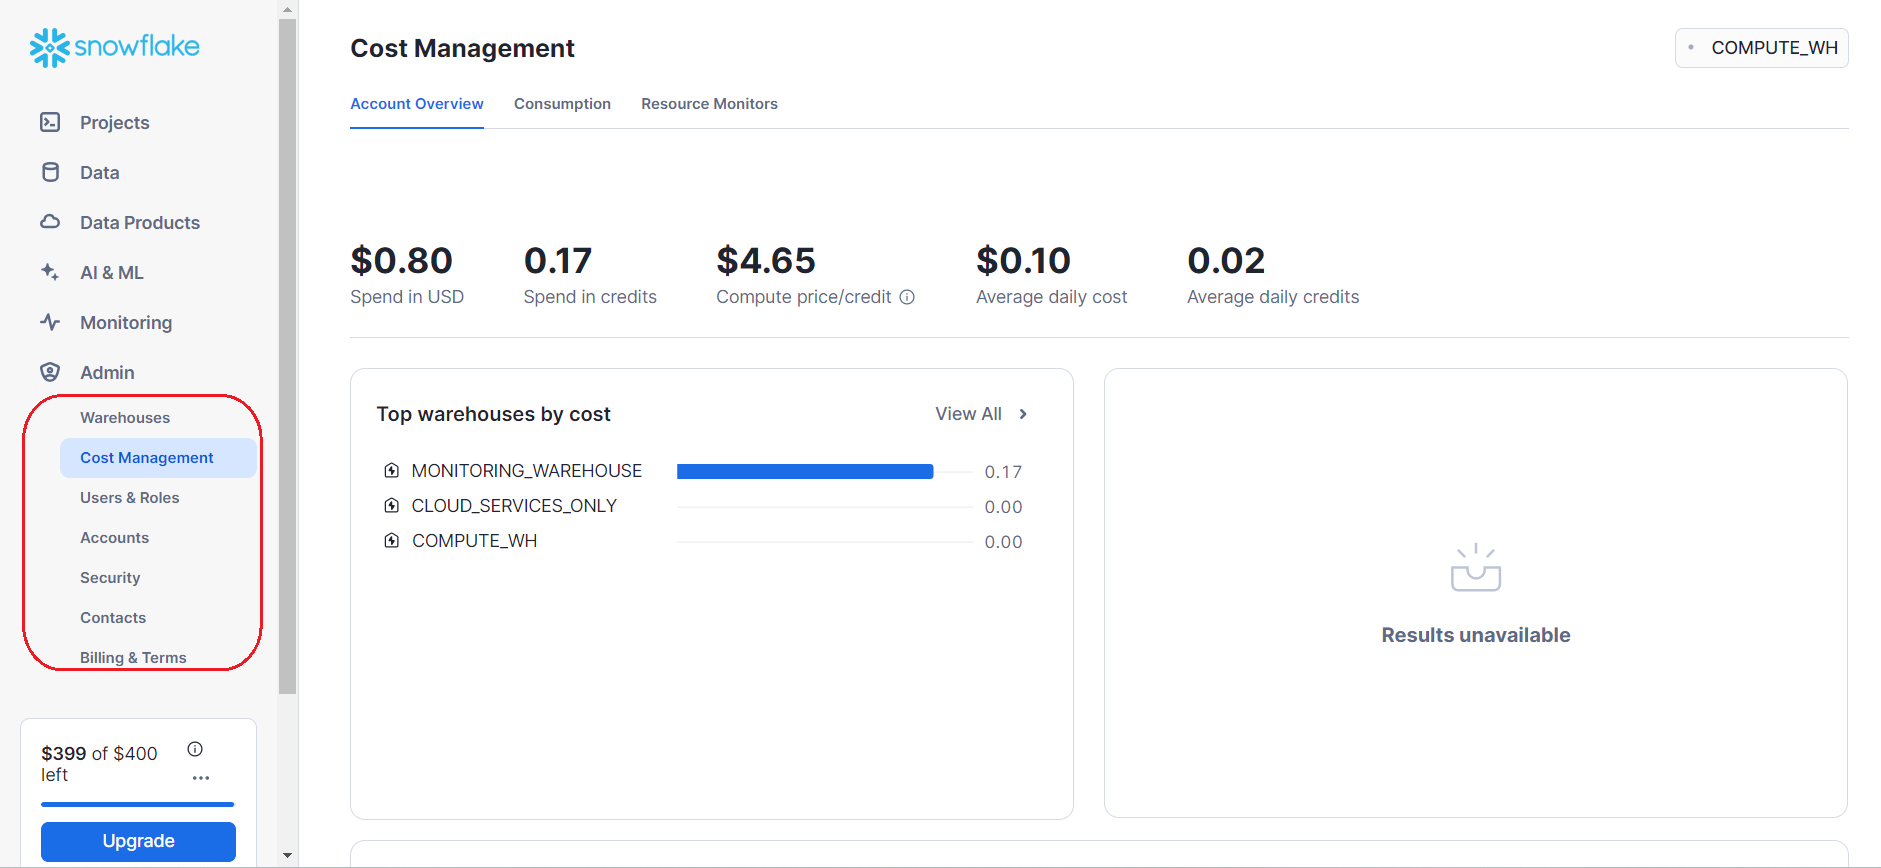
\includegraphics[width =13cm, height=7.5cm]{img/captures/account_usage}
            \caption{Snowflake account usage dashboard}
            \label{fig:SAU}
            \end{figure}
        %fin
    \item\textbf{Snowflake Information Schema :} est une collection de vues système qui fournissent des métadonnées sur les objets et les opérations effectuées dans un compte Snowflake. 
    Ces vues offrent une granularité élevée pour examiner les détails des requêtes SQL exécutées, les performances des entrepôts de données et d'autres aspects des opérations Snowflake. 
    \par La figure \textbf{\ref{fig:info}} suivante illustre une partie de cette vue:
        %code image
            \begin{figure}[H]
            \centering
            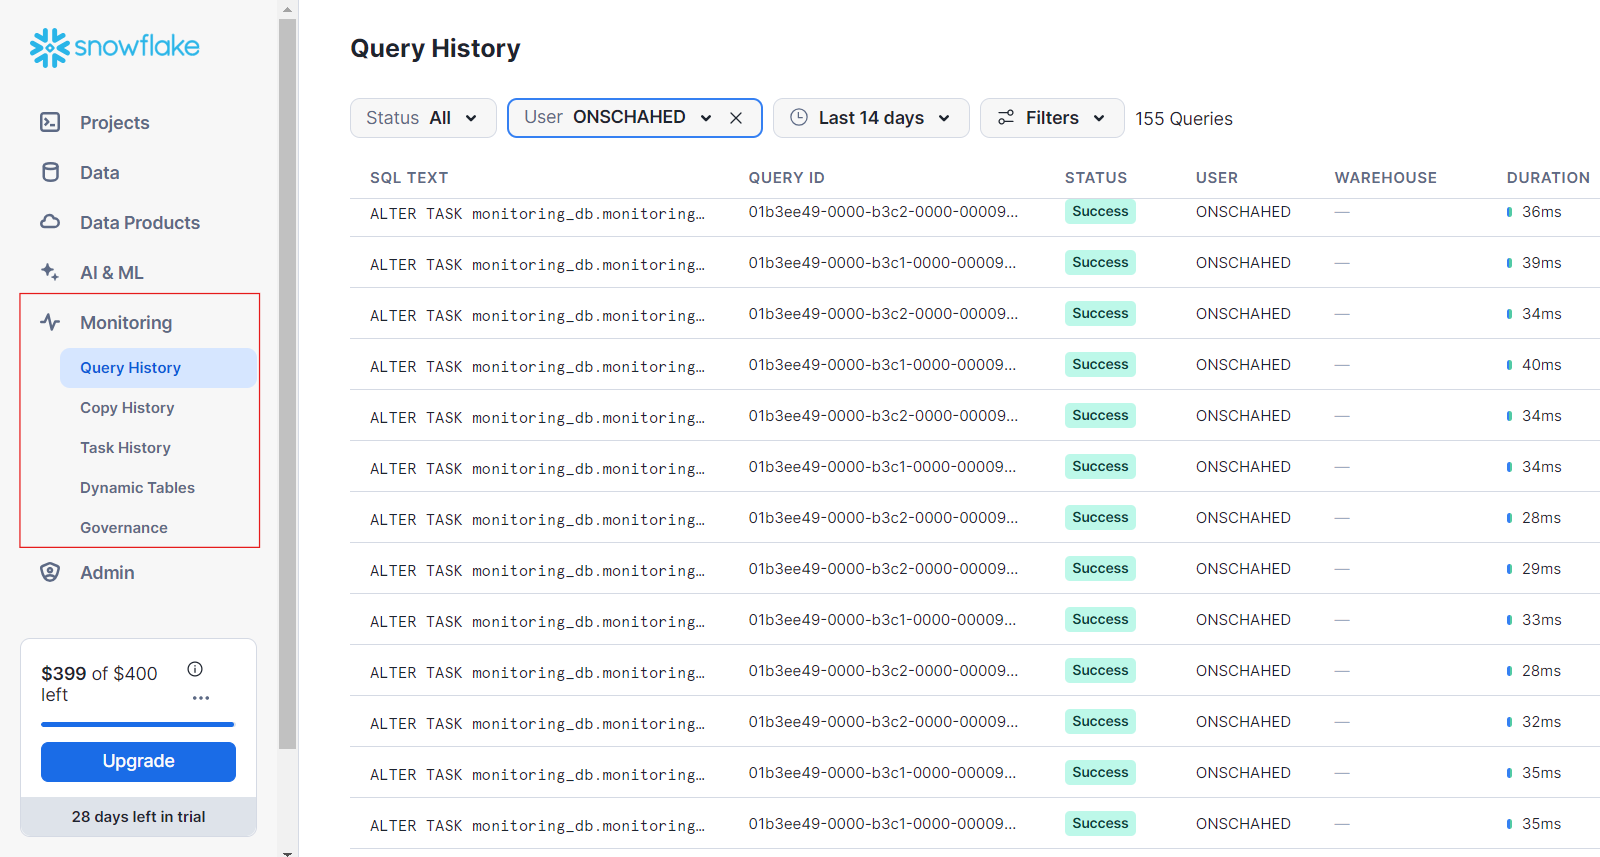
\includegraphics[width =13cm, height=7.5cm]{img/captures/info}
            \caption{Snowflake account usage dashboard}
            \label{fig:info}
            \end{figure}
        %fin
    \item\textbf{Google BigQuery :} est une autre option populaire pour le stockage et l'analyse des données dans le cloud. 
    Il offre des fonctionnalités avancées telles que le traitement massivement parallèle et la capacité à exécuter des requêtes SQL complexes sur de grands ensembles de données. 
    \par La figure \textbf{\ref{fig:BQ}} suivante illustre une partie de tableau de bord de BigQuery :
        %code image
            \begin{figure}[H]
            \centering
            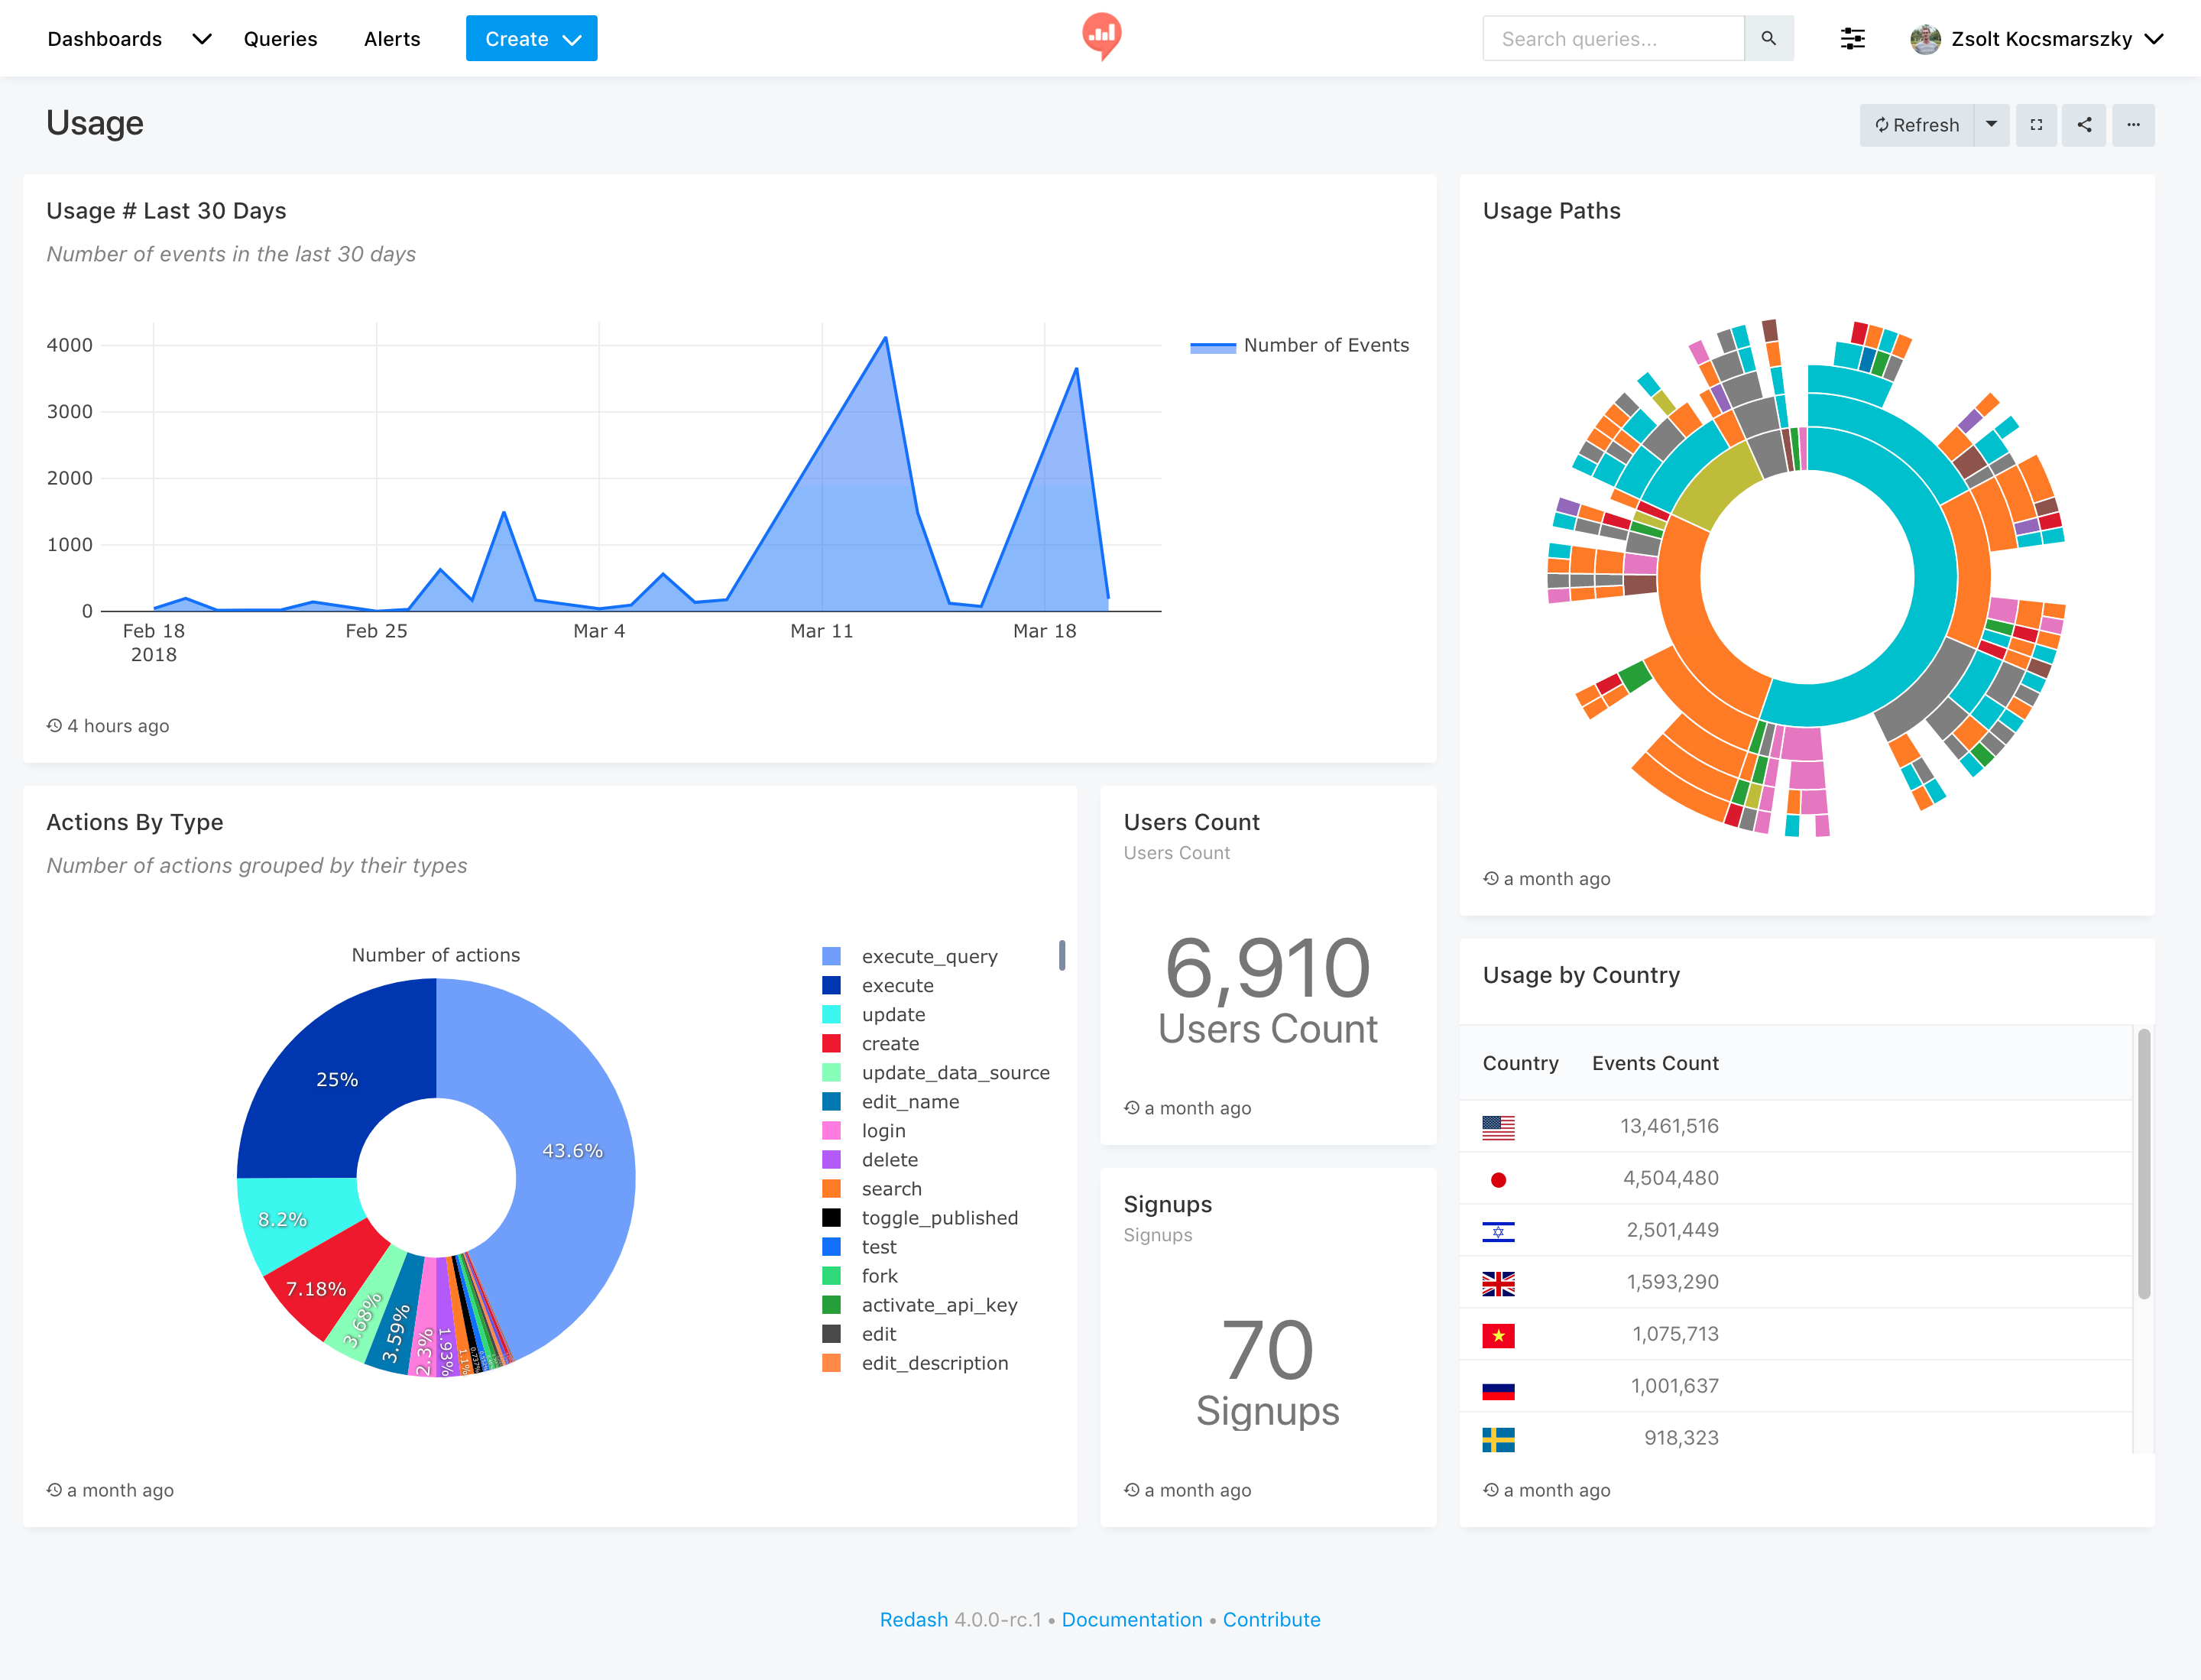
\includegraphics[width =13cm, height=7.5cm]{img/captures/bigquery}
            \caption{Tableau de bord de <<Google BigQuery>>}
            \label{fig:BQ}
            \end{figure}
        %fin

    \item\textbf{Amazon Redshift :} est un entrepôt de données cloud basé sur PostgreSQL, conçu pour gérer de gros volumes de données et exécuter des analyses complexes.
    Il offre des performances élevées et une extensibilité, mais son modèle de tarification basé sur l'utilisation des ressources peut entraîner des coûts supplémentaires pour les entreprises.
    \par La figure \textbf{\ref{fig:RS}} suivante illustre le tableau de bord de ResShift:
        %code image
            \begin{figure}[H]
            \centering
            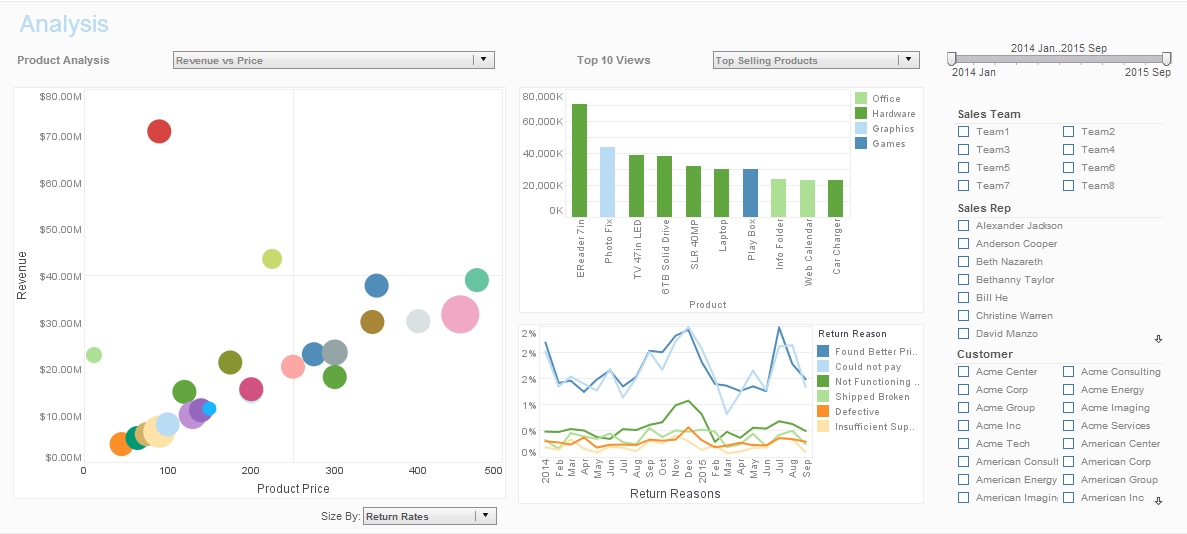
\includegraphics[width =13cm, height=7.5cm]{img/captures/redshift}
            \caption{Tableau de bord de "Amazon Redshift"}
            \label{fig:RS}
            \end{figure}
        %fin
\end{itemize}
\subsubsection{Critique de l'existant}
\par Dans cette section, nous allons examiner de manière critique les solutions actuellement utilisés dans le domaine de l'analyse de données, afin de fournir une base solide pour concevoir une solution qui surmonte les limitations et offre une valeur ajoutée significative à nos parties prenantes.
\begin{itemize}
    \item\textbf{Complexité des solutions : }les solutions de surveillance existants, comme le Snowflake Information Schema, sont souvent complexes à utiliser et nécessitent des compétences techniques avancées pour interpréter les données fournies. 
    Cette complexité peut rendre difficile la compréhension des métriques et la prise de décisions éclairées par les équipes opérationnelles ;
    (par exemple dans un flux de travail si une certaine tache est échouée, les indicateurs disponibles sur snowflake ne peuvent pas identifier ou exactement le workflow est suspendu de façon à rendre les choses plus compliqué pour les utilisaturs de Snowflake de détecter les anomalies si ils savent pas comment le manipuler techniquement.)

    \item\textbf{Personnalisation limitée : }les options de personnalisation offertes par les outils existants sont souvent limitées. 
    Par exemple, Google BigQuery propose des fonctionnalités avancées, mais la personnalisation des tableaux de bord et des rapports est restreinte. Cela peut être un obstacle pour les entreprises ayant des besoins spécifiques en matière de surveillance et d'analyse des performances ;

    \item\textbf{Coûts supplémentaires : }certains outils, comme Amazon Redshift, peuvent entraîner des coûts supplémentaires importants pour les entreprises. La tarification basée sur l'utilisation des ressources peut rapidement augmenter, surtout si les entreprises ne surveillent pas activement leur utilisation. Cela peut constituer une barrière financière pour les petites et moyennes entreprises souhaitant utiliser ces outils de surveillance ;

\end{itemize}

\subsection{Objectif du projet}
\par  L'objectif principal de ce projet est de propulser les opérations Snowflake d'Avaxia Group vers de nouveaux sommets en termes de performance, de rentabilité et d'efficacité. 
Le développement de cette nouvelle plateforme de surveillance aidera l'équipe d'Avaxia à surmonter ces défis majeurs.
\par Grâce à cette initiative, Avaxia Group pourra optimiser ses processus, réduire les coûts opérationnels et améliorer la qualité des services offerts à ses clients. En effet, cette nouvelle plateforme 
permettra de détecter rapidement les problèmes de performance, d'anticiper les besoins en ressources et de garantir une gestion plus efficace des opérations.
\subsection{Solution proposée}
\par Notre solution repose sur la conception et l'implémentation d'un système de surveillance et d'optimisation des opérations exhaustif. 
Cette solution se repartie en plusieurs composants clés, chacun ciblant des aspects spécifiques des problématiques identifiées:

\begin{itemize}
    \item La mise en place des stratégies de monitoring en temps réel cela permettra d'identifier rapidement les problèmes de performance et de prendre des mesures correctives efficaces ;
    \item le développement d'outils d'analyse avancée des coûts qui aiderent nos utilisateurs finaux à mieux comprendre ses dépenses et à trouver des opportunités d'optimisation pour 
    réduire les coûts tout en maintenant des performances élevées ;
    \item Développement des tableaux de bord interactifs et riches en informations pour permettre à Avaxia Group et à ses clients de surveiller en temps réel les performances de leurs opérations Snowflake. 
    Ces tableaux de bord fourniront des indicateurs clés de performance, des graphiques et des visualisations pour faciliter la détection des anomalies et la prise de décisions éclairées ;
    \item Utilisation de techniques d'analyse avancée des données opérationnelles pour permettre aux utilisateurs  d'identifier les opportunités d'amélioration et d'optimisation de leurs opérations, 
    renforçant ainsi leur compétitivité et leur efficacité ;
    \item Développement d'algorithmes d'optimisation des requêtes SQL afin de de réduire les temps d'exécution et de minimiser les goulets d'étranglement dans l'utilisation des ressources de Snowflake.
\end{itemize}


\section{Choix méthodologique}
\par Dans le but d'aboutir à une solution de qualité qui répond aux besoins exigés dans des
temps et des coûts prévisibles, le choix du processus de développement convenable est
une phase primordiale dans tout projet. Nous devons appliquer une méthode rigoureuse
sur la conduite de notre projet.
\subsection{Différence entre Scrum et Kanban}
\par La table \textbf{1.1} résume une comparaison entre les méthodes agiles de gestion des projets \textbf{Scrum} et \textbf{Kanban} :
\begin{table}[H]
    \centering
    \begin{tabular}{|p{3.5cm}|p{6cm}|p{6cm}|}
        \hline
        \rowcolor{blue!18}\textbf{\hbox{Point de comparaison}} & \textbf{Scrum} & \textbf{Kanban} \\
        \hline
        \textbf{Origine} & Développement logiciel & \hbox{ Fabrication Lean (Lean Manufacturing)} \\
        \hline
        \textbf{Idéologie} & Apprendre de ses expériences,\par s'organiser et hiérarchiser, et réfléchir à ses réussites et ses échecs afin de s'améliorer en permanence & Utiliser des visuels pour améliorer le travail en cours \\
        \hline
        \textbf{Cadence} & Sprints réguliers et à durée déterminée (à savoir, deux semaines) & Flux continu \\
        \hline
        \textbf{Bonnes pratiques }& Planification du sprint, sprint, mêlée \par quotidienne (Daily Scrum), revue du sprint, rétrospective du sprint & Visualiser le flux de travail, limiter le travail en cours, gérer le flux, intégrer des boucles de rétroaction \\
        \hline
        \textbf{Rôles }& Product Owner, Scrum Master, équipe de développement & Aucun rôle requis \\
        \hline
        \textbf{Utilisation des tableaux} & Un tableau Scrum est nettoyé et recyclé après chaque sprint & Un tableau Kanban est utilisé tout au long du cycle de vie d'un projet \\
        \hline
        \textbf{Nombre des tâches }& Un tableau Scrum possède un nombre \par de tâches définies ainsi que des\par échéances strictes pour les effectuer&
        Les tableaux Kanban sont plus flexibles en termes de tâches et d'échéances. Les tâches peuvent être hiérarchisées à nouveau, réassignées ou mises à jour si besoin. \\
        \hline
       
    \end{tabular}
    \label{tab:difference}
\caption{Comparaison entre les méthodes de gestion du projet Scrum et Kanban }
\end{table}

\subsection{Justification de choix}
\par Notre choix de Kanban comme étant pour la gestion de notre projet est le fruit d'une réflexion stratégique minutieuse. 
En effet, Kanban, qui tire son origine du terme japonais signifiant << tableau >>\cite{origine}, se démarque par sa flexibilité, sa transparence et sa focalisation sur l'amélioration constante.

\par Dans le cadre de notre projet, Kanban s'impose naturellement comme le choix optimal. 
Cette méthode permet une gestion visuelle et en temps réel des tâches et des flux de travail, une caractéristique cruciale pour un projet centré sur l'analyse de données et la visualisation.
 Chaque étape de notre processus, de la collecte des données à la présentation des résultats, trouve une représentation claire et concise dans le tableau Kanban.

\par De surcroît, Kanban promeut une approche itérative et progressive, parfaitement en harmonie avec notre objectif d'amélioration continue. 
Elle autorise une gestion fluide et adaptable des tâches, offrant la souplesse nécessaire pour ajuster notre plan en fonction des découvertes et des besoins changeants du projet.
\par En optant pour Kanban, nous mettons l'accent sur la transparence et la communication au sein de l'équipe. 
Chacun dispose d'une vision limpide de l'état d'avancement du projet, favorisant ainsi la collaboration et l'engagement de tous les membres.
\subsection{Le tableau Kanban}
\par Un tableau Kanban est un outil de gestion de projet Agile conçu pour aider à visualiser le travail, limiter le travail en cours et maximiser l'efficacité (ou le flux) \cite{kanban}.
\par Dans cette section, nous allons s'interésser à la spécificités des tableaux Kanban et leurs types

\subsubsection{Composants d'un tableau Kanban}
\par Dans cette partie, nous allons découvrir les composants d'un tableau Kanban. En effect, Les tableaux Kanban utilisent des cartes, des colonnes, des couloirs et des limites de travail 
en cours pour permettre aux équipes de visualiser et de gérer efficacement leurs flux de travail. Examinons ces principaux éléments plus en détail:

\begin{itemize}
    \item{\textbf{Carte Kanban}} : c'est une représentation visuelle des tâches. Chaque carte contient des informations importantes sur la tâche, telles que sa description, son statut d'avancement, les personnes impliquées, 
    les échéances, etc\cite{tableau} ;
    \item {\textbf{Colonne Kanban}}:chaque colonne une étape distincte du processus de travail. Les tâches traversent ces différentes colonnes au fur et à mesure 
    de leur avancement, jusqu'à ce qu'elles soient complètement terminées. Cette organisation visuelle permet de suivre et de maîtriser le flux de travail de manière efficace \cite{tableau} ;

    \item{\textbf{Couloir Kanban}} : sont des bandes horizontales pour séparer différents éléments tels que les activités, les équipes, les classes de service, etc.
     Ces bandes permettent d'organiser visuellement le tableau de manière plus granulaire et de mieux différencier les éléments qui le composent \cite{tableau} ;

     \item{\textbf{Limite de travail en cours}} : elles limitent la quantité maximum de tâches dans les différentes étapes du flux de travail.
      Elles vous permettent de terminer des tâches plus rapidement en aidant votre équipe à ne concentrer que sur les tâches en cours \cite{tableau};

    \item{\textbf{Point d'engagement}} : un point d'engagement est un point dans le processus de travail auquel une tâche est prête à être incorporée au système \cite{tableau} ;
    \item{\textbf{Point de livraison }} : point du flux de travail auquel une tâche est considérée comme terminée \cite{tableau}.
\end{itemize}
    \subsubsection{Types des tableaux Kanban}
    \par Les tableaux Kanban peuvent être divisés en plusiedeux types :
    \begin{enumerate}
        \item[1-]\textbf{Un tableau Kanban physique }: est la forme la plus basique, les équipes utilisent des Post-its (représentant des tâches) et un tableau blanc (ou en liège). 
        Les phases de travail sont représentées par des colonnes et les Post-its sont déplacés d'une étape à une autre \cite{tableau}.
        \item[2-]\textbf{Un tableau Kanban numérique }: est une solution logicielle, ce qui le rend plus accessible que son pendant physique. Il peut vous fournir une visibilité sur la progression du travail depuis quasiment n'importe où, ce qui facilite la collaboration d'équipe. 
        Certaines solutions numériques s'avèrent très souples, permettant aux responsables de suivre plusieurs flux de travail et d'organiser leur travail en différentes catégories \cite{tableau}.
    \end{enumerate}
\par Pour la gestion de notre projet, nous avons choisi \textbf{<< Trello >>} qui est une platforme rapide et simple pour la création d'un tableau Kanban numérique.


\par En résumé, la méthode Kanban s'impose comme un choix stratégique judicieux pour notre projet, offrant un cadre solide pour une gestion efficace, transparente et itérative, tout en servant l'objectif fondamental d'amélioration continue de la performance de l'équipe.

\section*{Conclusion}
\addcontentsline{toc}{section}{Conclusion}
   À la clôture de ce chapitre initial, nous avons jeté les fondements pour la compréhension complète de la sphère du projet. Cette phase est cruciale pour cadrer les enjeux et les perspectives qui guident notre travail. Dans le prochain chapitre, nous explorerons en détail l'analyse et la spécification des besoins, une étape essentielle pour la réalisation de notre projet.
        \clearpage
        
        \chapter{Analyse et spécification des besoins}

\section*{Introduction}
\addcontentsline{toc}{section}{Introduction }
    \par {\huge L}a réussite de toute étude dépend de la qualité de la phase de démarrage. 
    De ce fait, l'étape d'analyse des besoins constitue la base de départ de notre travail 
    ainsi qu'une étape déterminante pour la suite. 
    Dans ce chapitre, nous évoquerons tout d'abord les besoins fonctionnels et non
    fonctionnels de notre solution. Ensuite Nous définissons clairement le flux de travail 
    qu'oon va élaborer tout au long de ce projet. Finalement, nous allons dresser le backlog produit qui contient toutes les fonctionnalités que nous
    allons utiliser comme étant la base essentielle de la phases suivantes de planification et de développement.
    \section{Concepts de base}

    Dans cette section, nous définissons et expliquons les principaux concepts et technologies essentiels à notre projet de monitoring des opérations sur Snowflake. La compréhension de ces concepts est cruciale pour saisir le fonctionnement et les objectifs de notre solution.
    
    \subsection{La platforme Snowflake }
    
    \textbf{Snowflake} est une plateforme de data warehousing cloud conçue pour le stockage et l'analyse de données à grande échelle.
    Elle offre des capacités de traitement massivement parallèle, permettant une scalabilité pratiquement illimitée. 
    Snowflake se distingue par la séparation des couches de stockage et de calcul, offrant ainsi des avantages en termes de flexibilité, de performance et de coût \cite{snowflake}.
    
    \textbf{Fonctionnalités clés de Snowflake :}
    \begin{itemize}
        \item \textit{Stockage des données} : Utilisation de la compression et de la partition pour optimiser le stockage ;
        \item \textit{Calcul élastique} : Possibilité de redimensionner les ressources de calcul en fonction des besoins ;
        \item \textit{Partage sécurisé des données} : Facilite le partage des données entre différentes organisations tout en assurant la sécurité ;
        \item \textit{Support SQL complet} : Prise en charge des commandes SQL standards pour la manipulation des données.
    \end{itemize}
    
    \subsection{Directed Acyclic Graph (DAG)}
    
    Un \textbf{DAG (Directed Acyclic Graph)} est une structure de données qui représente un ensemble de tâches et leurs dépendances sous forme
     de graphe dirigé sans cycles\cite{dagdef}. Dans le contexte des pipelines de données, un DAG est souvent utilisé pour définir les étapes de traitement des données et leur ordre d'exécution.
    
    \textbf{Utilisation des DAGs :}
    \begin{itemize}
        \item \textit{Planification des tâches} : Détermination de l'ordre dans lequel les tâches doivent être exécutées ; 
        \item \textit{Gestion des dépendances} : Assure que les tâches dépendantes sont exécutées dans le bon ordre ;
        \item \textit{Parallélisme} : Permet l'exécution simultanée de tâches indépendantes.
    \end{itemize}
    
    \subsection{Solution de Monitoring}
    
    Une \textbf{solution de monitoring} est un ensemble d'outils et de pratiques conçus pour surveiller les performances,
     la disponibilité et la santé des systèmes informatiques. Elle collecte, analyse et affiche des métriques et des logs 
     pour aider les administrateurs à détecter et résoudre les problèmes\cite{monitoring}.
    
    \textbf{Caractéristiques d'une solution de monitoring efficace :}
    \begin{itemize}
        \item \textit{Collecte de métriques en temps réel} : Surveillance continue des performances et des ressources ;
        \item \textit{Alertes et notifications} : Système d'alerte en cas d'anomalies ou de dépassement de seuils définis ;
        \item \textit{Visualisation des données} : Tableaux de bord interactifs pour l'analyse des métriques et des tendances ;
        \item \textit{Reporting} : Génération de rapports détaillés pour le suivi et l'analyse historique.
    \end{itemize}
    
    \subsection{Analyse des Données}
    
    L'\textbf{analyse des données} est la science qui consiste à examiner les données pour en tirer des informations permettant de prendre des décisions ou d'approfondir les connaissances sur divers sujets \cite{analyse}. Elle vise à comprendre et exploiter les données pour des prises de décision éclairées.
    
    \textbf{Étapes de l'analyse des données :}
    \begin{itemize}
        \item \textit{Collecte des données} : Réunir les données pertinentes à partir de diverses sources.
        \item \textit{Préparation des données} : Nettoyage et transformation des données brutes en un format utilisable.
        \item \textit{Modélisation} : Utilisation de modèles statistiques et algorithmiques pour analyser les données.
        \item \textit{Interprétation et visualisation} : Présentation des résultats sous forme de graphiques et de rapports compréhensibles.
    \end{itemize}
    
    \subsection{L'ingénierie des données}
    
    L'\textbf{ingénierie des données} est la discipline consistant à concevoir, construire et maintenir des systèmes et des architectures pour collecter, stocker et analyser des données. Elle se concentre sur la création de l'infrastructure permettant l'exploitation des données par les analystes pour des prises de décision éclairées.
    
    \textbf{Responsabilités du l'ingénierie des données :}
    \begin{itemize}
        \item \textit{Conception de pipelines de données} : Définir et implémenter les processus de collecte, de transformation et de stockage des données.
        \item \textit{Gestion des bases de données} : Assurer la performance, la sécurité et l'intégrité des bases de données.
        \item \textit{Optimisation des requêtes} : Améliorer les requêtes pour une exécution plus rapide et efficace.
        \item \textit{Intégration de données} : Combiner les données provenant de diverses sources pour une vue unifiée.
    \end{itemize}
    
    Cette section vise à établir une compréhension claire des concepts et des technologies essentiels utilisés dans notre projet. Cela permettra de mieux appréhender les choix de conception et les décisions techniques prises tout au long du développement de la solution de monitoring des opérations sur Snowflake.
    
\section{Capture des besoins}
\par La capture des besoins est une phase fondamentale dans la réalisation du projet puisque elle doit
permettre aux utilisateurs finaux et au maître d'ouvrage de bien exprimer leurs besoins et de bien
comprendre les fonctionnalités que le système va fournir.
    % Une sous section
    \subsection{Besoins fonctionnels}
        \par Cette section décrit en détail les besoins fonctionnels du projet de monitoring des opérations Snowflake.
        Ces besoins ont été identifiés à partir des exigences de l'entreprise et des utilisateurs, et sont essentiels pour le développement d'une solution efficace et adaptée aux besoins de l'entreprise.
    \begin{itemize}
            \item \textbf{La collecte automatique des données de Snowflake} :
            Le système doit être capable de collecter automatiquement les données de Snowflake, y compris les requêtes exécutées et leurs informations, l'utilisation des ressources (CPU, mémoire, stockage), les bases de données et leurs objets ( tâches, tables, tubes, etc. ), les statistiques sur les entrepôts de données, etc... ;
            
            \item \textbf{La surveillance en temps réel des requêtes SQL} :
            Le système doit surveiller en temps réel les requêtes SQL exécutées sur Snowflake, enregistrant ces informations détaillées, les erreurs éventuelles, et en identifiant les requêtes lentes ou mal optimisées ;
            
            \item \textbf{La surveillance en temps réel des entrepôts de données} :
            Le système doit surveiller en temps réel les métriques des entrepôts de données, y compris l'utilisation de l'espace disque, la répartition de la charge de travail et la consommation de ressources ;
            
            \item \textbf{L'élaboration des tableaux de bord interactifs pour les métriques clés} :
            Le système doit fournir des tableaux de bord interactifs permettant de visualiser les métriques clés de performance de Snowflake, y compris les temps de réponse des requêtes, l'utilisation des ressources et les statistiques sur les entrepôts de données ;
            
            \item \textbf{Suivi des tâches et leurs DAGs} :
            Le système doit permettre le suivi des tâches et des DAGs exécutées dans Snowflake, enregistrant les étapes effectuées, les tous leurs informations et les erreurs éventuelles ;
            
            \item \textbf{La surveillance de l'utilisation des crédits} :
            Le système doit surveiller l'utilisation des crédits de calcul sur Snowflake, enregistrant les crédits utilisés par chaque requête ou chaque tâche, ainsi que les tendances d'utilisation au fil du temps ;
            
            \item \textbf{La surveillance des utilisateurs et des accès} :
            Le système doit suivre l'activité des utilisateurs sur Snowflake, en enregistrant leurs requêtes exécutées, les objets accédées et les autorisations utilisées ;
            
            \item \textbf{Alertes et notifications en cas d'anomalies} :
            Le système doit générer des alertes et des notifications en temps réel en cas d'anomalies ou de situations critiques, telles qu'une augmentation soudaine du temps de réponse des requêtes ou une utilisation anormale des ressources; 
            
            \item \textbf{Personnalisation des tableaux de bord} :
            Le système doit permettre aux utilisateurs de personnaliser les tableaux de bord en fonction de leurs besoins spécifiques, en sélectionnant les métriques à afficher et en configurant les seuils d'alerte.
        \end{itemize}        
    % Une deuxième sous section
    \subsection{Besoins non fonctionnels}
  \par Cette section détaille les besoins non fonctionnels du projet de monitoring des opérations Snowflake. 
  Ces besoins concernent principalement les aspects de performance, de sécurité, d'évolutivité et d'expérience utilisateur de la solution. 
  Ils sont essentiels pour garantir que le système répond aux attentes de l'entreprise en termes de qualité et de fiabilité.

  \begin{itemize}
        \item\textbf{Besoins en Performance}

                \begin{enumerate}
                    \item[1.] \textbf{Temps de réponse} : Le système doit fournir des temps de réponse rapides pour l'affichage des tableaux de bord, afin de garantir une expérience utilisateur fluide ;
                    
                    \item[2.] \textbf{Évolutivité} : Le système doit être capable de gérer une grande quantité de données et de trafic sans compromettre ses performances, en s'adaptant de manière transparente à l'augmentation de la charge.
                \end{enumerate}
    
        \item\textbf{Besoins en Sécurité}
    
                \begin{enumerate}
                    \item[1.] \textbf{Confidentialité des données} : Le système doit garantir la confidentialité des données collectées, en assurant leur cryptage lors du stockage et de la transmission ;
                    
                    \item[2.] \textbf{Authentification et autorisation} : Le système doit mettre en place des mécanismes d'authentification robustes pour vérifier l'identité des utilisateurs 
                    et des administrateurs, ainsi que des contrôles d'autorisation pour limiter l'accès aux données sensibles.
                \end{enumerate}
    
        \item\textbf{Besoins en Disponibilité}
    
                \begin{enumerate}
                    \item[1.] \textbf{Disponibilité} : Le système doit être disponible en permanence, avec un temps de fonctionnement maximal et une reprise rapide en cas de panne ;
                    
                    \item[2.] \textbf{Tolérance aux pannes} : Le système doit être capable de résister aux pannes matérielles ou logicielles, en assurant la redondance des composants critiques et la sauvegarde des données.
                \end{enumerate}
    
        \item\textbf{Besoins en Expérience Utilisateur}
    
                \begin{enumerate}
                    \item[1.] \textbf{Facilité d'utilisation} : Le système doit être intuitif et convivial, avec une interface utilisateur bien conçue et une navigation facile ;
                    
                    \item[2.] \textbf{Personnalisation} : Le système doit permettre aux utilisateurs de personnaliser leur expérience, en configurant les préférences d'affichage et les paramètres de notification.
                \end{enumerate}
        \item \textbf{Archivage des données: }Les données historiques doivent être archivées de manière efficace pour garantir l'intégrité des données.
  \end{itemize}
  \subsection{Diagramme de cas d'utilisation global}
  \par Le diagramme de cas d'utilisation permet d'identifier les possibilités d'interaction entre le système et les acteurs (intervenants extérieurs au système), c'est-à-dire toutes les fonctionnalités
  que doit fournir le système. L'idée forte est de dire que l'utilisateur d'un système logiciel a un objectif quand il utilise le système \cite{use_case}.
  \par La figure \textbf{\ref{fig:use}} qui suit représente le diagramme de cas d'utilisation global de notre système:     
    %code image
        \begin{figure}[H]
            \centering
            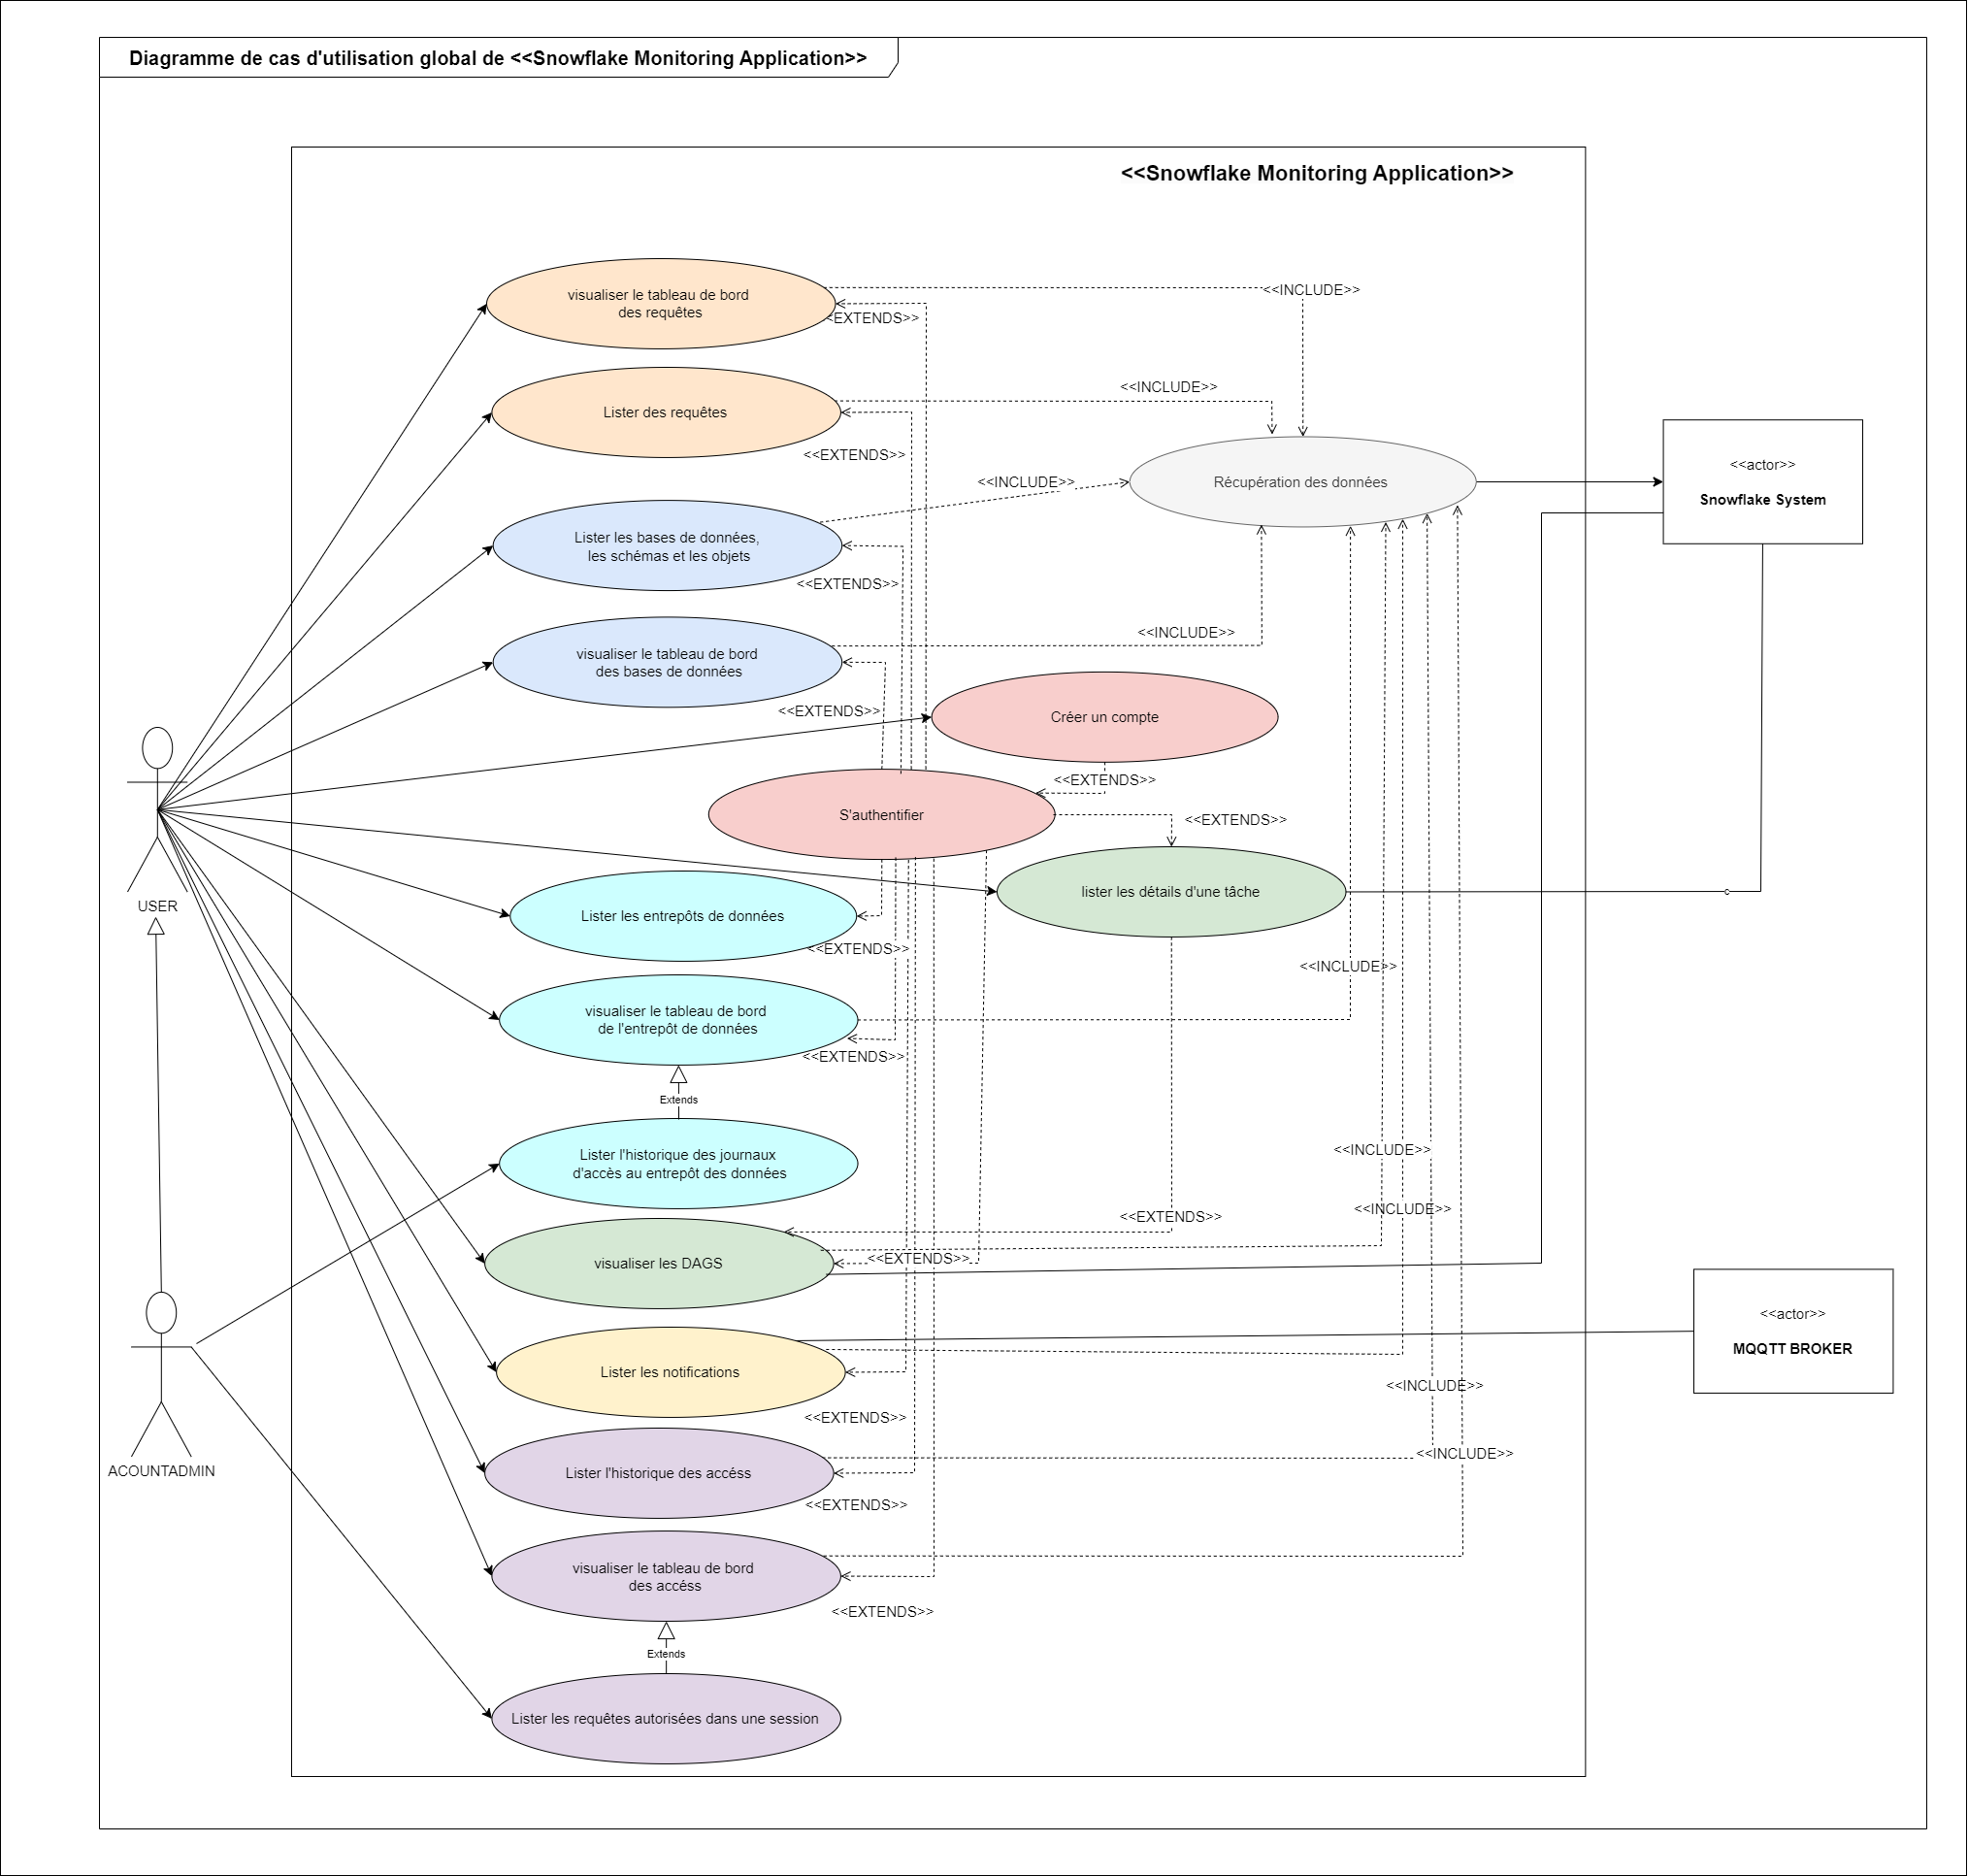
\includegraphics[ width=1\linewidth]{img/conception/use_case.png}
            \caption{Diagramme de cas d'utilisation globale <<Snowflake Monitoring Application>>}
            \label{fig:use}
            \end{figure}
\par Le diagramme de cas d'utilisation global présenté ci-dessus offre une vue d'ensemble des interactions potentielles entre les utilisateurs et le système de monitoring Snowflake. 
En identifiant clairement les objectifs des utilisateurs et les fonctionnalités requises, ce diagramme joue un rôle crucial dans la définition des exigences du système. 
En somme, ce diagramme est un outil essentiel pour garantir que le système final réponde aux besoins des utilisateurs de manière efficace et cohérente.


  \section{Flux de travail}
  \par Durant la réalisation de notre projet, ce processus a été notre fil conducteur, nous permettantpermettons de passer par plusieurs étapes clés pour atteindre notre objectif. 
La figure \textbf{\ref{fig:BPMN}} suivante illustre notre processus métier :
    %code image
        \begin{figure}[H]
        \centering
        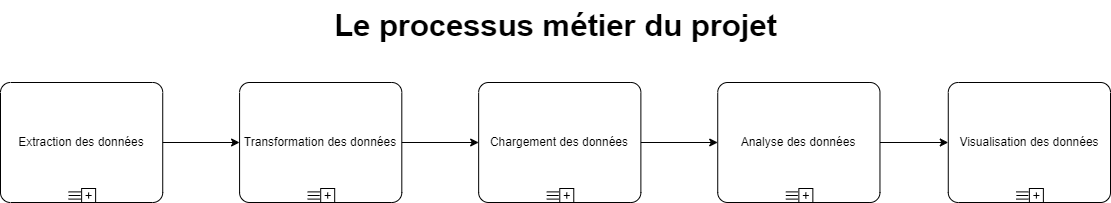
\includegraphics[width=1\linewidth, height=3.5cm]{img/conception/BPMN.png}
        \caption{Processus métier du projet}
        \label{fig:BPMN}
        \end{figure}
    %fin
  \par Maintenant, nous allons explorer en détail le flux de travail que nous avons suivi, en soulignant l'importance de chaque étape et en expliquant comment elles se sont complétées pour aboutir à une solution complète. 
  Ensuite, nous examinerons chaque étape de manière approfondie pour comprendre comment elles ont contribué à notre succès global.
  \par Passons maintenant à l'examen détaillé de chacune de ces étapes.

  \begin{itemize}
  
  \item \textbf{Extraction des données :}
  \par Cette étape consistait à recueillir des informations provenant des différentes vues du système Snowflake. 
  L'objectif principal est de collecter les données nécessaires à notre analyse. 
  L'extraction de données est une phase cruciale dans l'ingénierie des données, car elle constitue le point de départ de tout projet d'analyse. 
  Les techniques d'extraction comprenaient des requêtes SQL avancées et l'automatisation des processus d'extraction pour garantir une collecte fiable et régulière.

  \item \textbf{Transformation des données :}
  \par L'objectif principal de cette étape est de nettoyer et structurer les données. Car, ces données brutes pouvaient contenir des erreurs, des doublons, des incohérences et/ou des valeurs manquantes. 
  Nous allons appliquer des techniques de nettoyage, telles que l'imputation des valeurs manquantes, la déduplication et la normalisation des données.
   De plus, des processus de transformation ont été utilisés pour convertir les données dans des formats appropriés pour l'étape suivante.

  \item \textbf{Chargement des données :}
  \par Une fois les données nettoyées et préparées, elles sont acheminées vers une base de données ou un entrepôt de données. Le chargement vise à stocker les données de manière centralisée pour une accessibilité et une analyse ultérieures.
   Cette phase garantit que les données sont correctement indexées, partitionnées et optimisées pour des requêtes rapides et efficaces.

  \item \textbf{Analyse des données :}
  \par Cette phase consiste à explorer les données pour en extraire des informations significatives. 
  L'analyse des données utilise des méthodes statistiques, des techniques de modélisation, des calculs de corrélation, etc., pour comprendre les tendances et les relations entre les données.
   Cette étape est essentielle pour transformer les données brutes en informations exploitables.

  \item \textbf{Visualisation des données :}
  \par L'analyse des données est souvent présentée de manière visuelle sous forme de tableaux de bord interactifs, de graphiques ou bien des diagrammes.En effet, ces visualisations permettent aux utilisateurs de comprendre rapidement les résultats de l'analyse. 

  \end{itemize}
  \par Ces phases constituent un flux de travail complet pour gérer les données, les transformer en informations exploitables et les présenter de manière efficace pour aider nos utilisateurs finaux à surveiller leurs données de manière concrète.

  \section{Le backlog du produit}
\par Le backlog de produit est destiné à recueillir tous les besoins du client pour l'équipe projet. Il contient la liste des fonctionnalités inclues dans un produit, ainsi que les éléments nécessitant l'intervention de l'équipe projet. Le backlog Scrum classe les éléments par priorité pour indiquer leur ordre de réalisation.\cite{blog}.

 \par Le backlog en KANBAN n'est pas si différent d'un backlog scrum en réalité. La différence réside surtout sur les règles de sa gestion \cite{BPK}.  
    
    \par la table \textbf{\ref{tab:backlog_produit}} suivante présente le backlog de produit de notre projet. 
%%%%%table
\begin{center}

    \begin{longtable}{|p{0.05\linewidth}|p{0.65\linewidth}|p{0.12\linewidth}|p{0.12\linewidth}|}
        \hline       
        \rowcolor{blue!18}\textbf{ID} & \textbf{User Story} &  \textbf{Priorité} & \textbf{Estimation (points)} \\
        \hline
        \endfirsthead
        US1 &  En tant qu'administrateur, je veux un tableau de bord global pour surveiller les performances générales de l'entrepôt de données, y compris les temps de réponse des requêtes, l'utilisation des ressources et les erreurs éventuelles. & Haute & 8 \\
        
        \hline
        
        US2 &  En tant qu'administrateur, je veux être en mesure de suivre en temps réel l'exécution des requêtes SQL sur la plateforme Snowflake, y compris les temps d'exécution, le nombre de lignes retournées et les plans d'exécution. & Haute & 10 \\
        
        \hline
        
        US3 &  En tant qu'administrateur, je veux surveiller l'utilisation des ressources (CPU, stockage, etc.) des bases de données pour identifier les goulots d'étranglement et les problèmes de capacité. & Haute & 9 \\
        
        \hline
        
        US4 &  En tant qu'administrateur, je veux recevoir des alertes en temps réel en cas de dégradation des performances de l'entrepôt de données afin de pouvoir réagir rapidement et résoudre les problèmes. & Haute & 8 \\
        
        \hline
        
        US5 & En tant qu'utilisateur, je veux surveillance la consommation de crédits, le coût par requête et l'utilisation des ressources au fil du temps. & Moyenne & 6 \\
        
        \hline
        
        US6 &  En tant qu'administrateur, je veux suivre l'activité des utilisateurs sur la plateforme Snowflake, y compris les requêtes exécutées, les tables accédées et les autorisations utilisées. & Moyenne & 7 \\
        
        \hline
        
        US7 &  En tant qu'administrateur, je veux être capable de gérer les sessions utilisateur actives, y compris la déconnexion des sessions inactives et la surveillance des sessions gourmandes en ressources. & Haute & 8 \\
        
        \hline
        
        US8 &  En tant qu'administrateur, je veux pouvoir définir des alertes personnalisées basées sur des seuils de performance spécifiques pour les requêtes, les ressources et les sessions. & Moyenne & 7 \\
        
        \hline
        
        US9 &  En tant que utilisateur, je veux accéder à des recommandations d'optimisation des requêtes SQL pour améliorer les performances et réduire les coûts. & Faible & 9 \\
        
        \hline
        
        US10& En tant qu'administrateur, je veux surveiller l'exécution des tâches planifiées (comme les pipelines de chargement) pour détecter les retards ou les échecs. & Haute & 21 \\
        
        \hline
        
        US11 & En tant qu'utilisateur, je veux pouvoir analyser les tendances historiques des performances pour identifier les schémas et les anomalies. & Moyenne & 8 \\
        
        \hline
        
        US12 & En tant qu'utilisateur, je veux s'authentifier d'une façon sécurisée pour accéeder a la platforme de monitoring & Moyenne & 5 \\
        
        \hline
        US13 & En tant qu'administrateur, je veux suivre en temps réelle l'execution des taches en temps réel avec une visualisation compléte du DAG, ainsi les différents états des tâches  & haute & 13 \\
        
        \hline
        US14 & En tant qu'administrateur, je veux suivre l'historique des journaux d'accès au entrepôt des données & haute & 9 \\
        
        \hline
        US15 & En tant qu'administrateur, je veux paramétrer les visualisations, les alertes, les limites du coûts selon les besoins ou/et les rôles & faible & 9 \\
        
        \hline
        
        \caption{Backlog de Produit}
        \label{tab:backlog_produit}
    \end{longtable}
    \par 

\end{center}
\par En conclusion, le backlog du produit joue un rôle essentiel dans notre projet en fournissant une vue d'ensemble claire et priorisée des fonctionnalités à développer et des tâches à accomplir. 
En utilisant la méthodologie Kanban, nous avons pu gérer efficacement ces éléments, ajuster nos priorités en temps réel et assurer une progression continue vers nos objectifs.

%%%%%table
\vspace{-1cm}
\section*{Conclusion}
\addcontentsline{toc}{section}{Conclusion}
 \par Ce chapitre a établi les fondations de notre projet.  Nous avons commencé par une introduction détaillée des concepts clés et des technologies qui sous-tendent notre solution, garantissant ainsi une compréhension solide de notre domaine d'application. 
 Ensuite, nous avons effectué les besoins fonctionnels et non fonctionnels, et présenté le diagramme de cas d'utilisation global pour illustrer les interactions entre utilisateurs et système. 

\par Nous avons également détaillé le flux de travail, de l'extraction à la visualisation des données, et élaboré un backlog de produit structuré et priorisé, 
garantissant une progression continue du projet. 
En résumé, ce chapitre a formalisé les bases nécessaires pour le développement et la mise en œuvre de notre solution de monitoring, assurant ainsi une réponse cohérente aux besoins des utilisateurs. Dans le prochain chapitre, nous explorerons les aspects architecturaux et conceptuels de notre projet.


        \clearpage
        
        \chapter{Architecture et conception}

\section*{Introduction}
\addcontentsline{toc}{section}{Introduction}
    \par Le troisième chapitre explore l'architecture du projet et sa étude conceptuelle. 
Nous allons justifier notre choix architectural et détaillrons la conception qui nous a ménné à la réalisation de notre solution.

\section{Étude architecturale}
    \par  L'étude architecturale joue un rôle central dans la conception et le déploiement d'une solution robuste et évolutive.
\subsection{Architecture logique}
\par Dans cette section, nous examinerons en profondeur l'architecture du système, couvrant à la fois ses dimensions logiques et physiques. Nous discuterons également des défis techniques et logiques rencontrés et des solutions déployées pour assurer une infrastructure solide et efficace.

\subsubsection{Architecture logique adoptée} 
\par Pour la mise en place de ce projet, nous avons délibérément opté pour \textbf{une architecture micro-services}, une décision dictée par des critères spécifiques qui s'accordent parfaitement avec les exigences de notre projet ainsi que les differentes parties prenantes.
 Cette architecture met en lumière les différents composantes fonctionnelles et explique comment ces composantes interagissent pour fournir une expérience utilisateur fluide et des analyses précises\cite{archi_log}. 
Cette derniére est illustrée par la figure \textbf{\ref{fig:arch_log}} suivante :
%code image
        \begin{figure}[H]
        \centering
        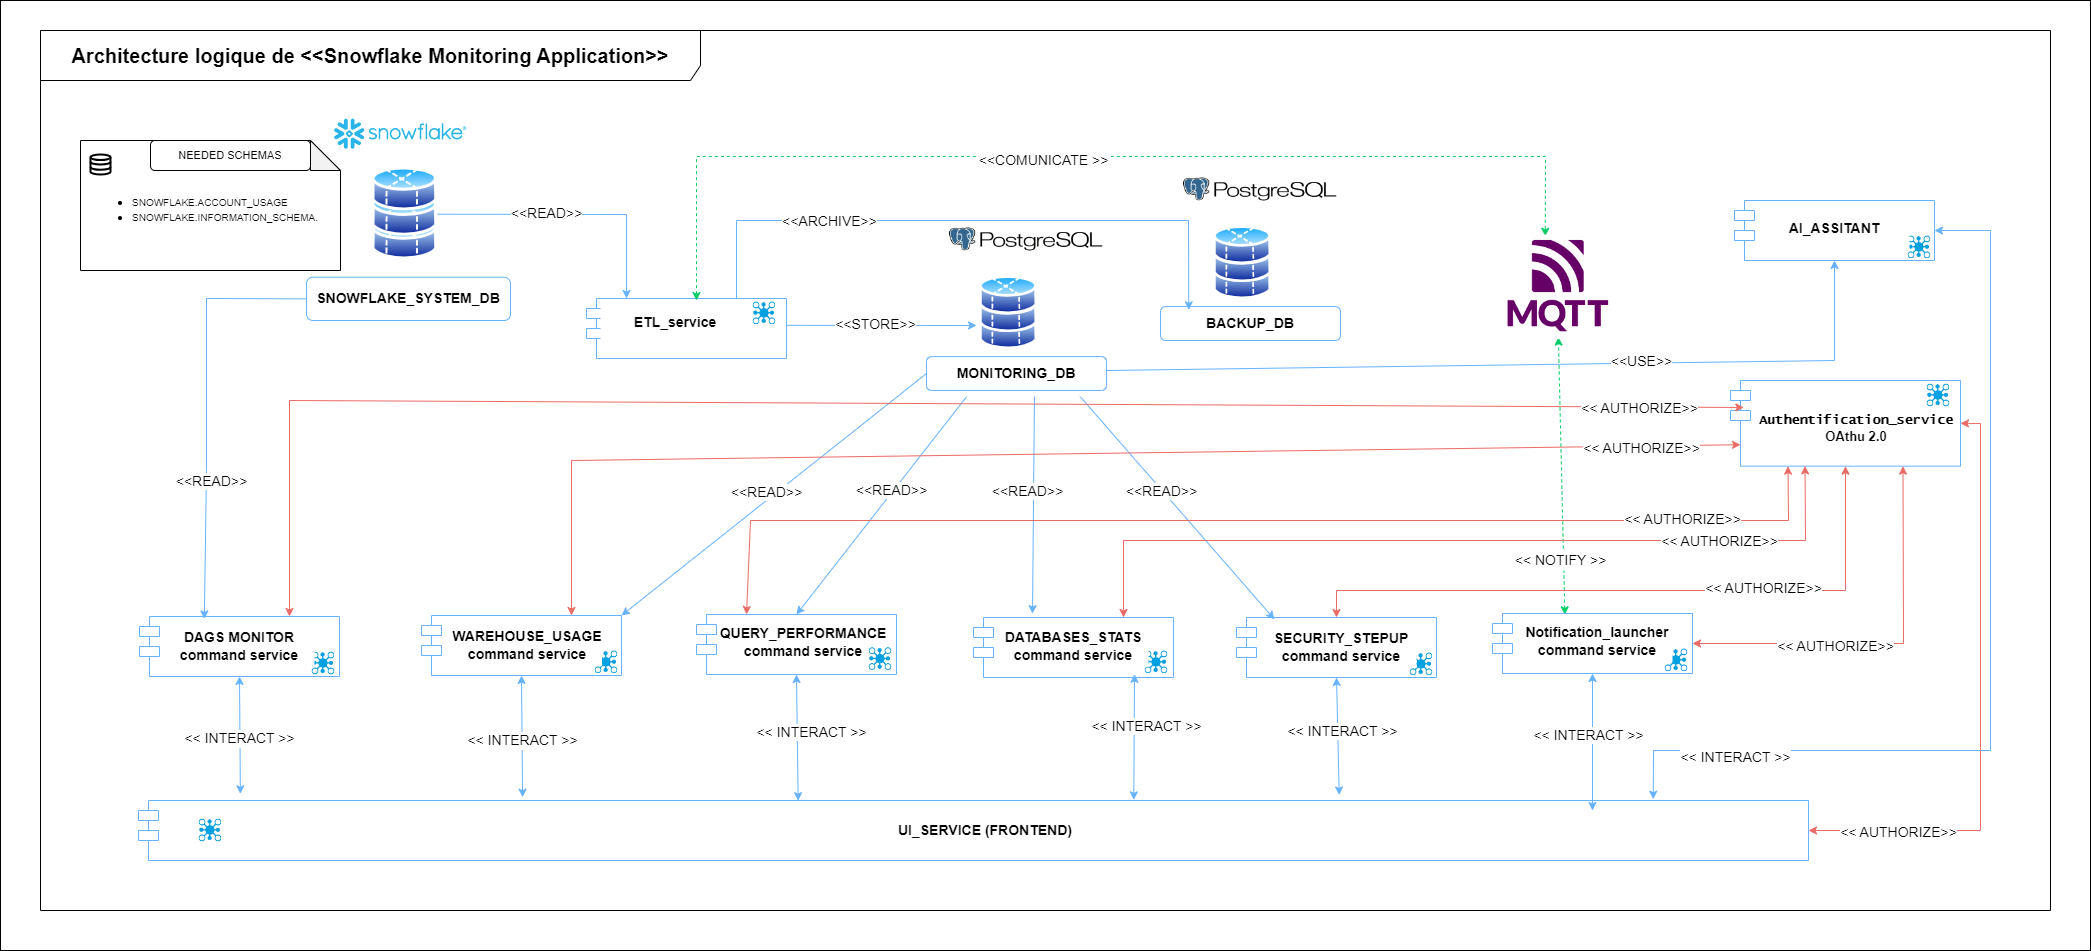
\includegraphics[width = 1\linewidth]{img/conception/archi.png}
        \caption{Architecture logique de <<Snowflake Monitoring Application>>}
    \label{fig:arch_log}
        \end{figure}
        %fin
    \par Notre architecture est repartie comme suit: 
    \begin{enumerate}

        \item[1.] \textbf{Couche des données:} 
                \begin{itemize}
                \item \textbf{Snowflake}: ce composant représente les vues sytémes de Snowflake telque <<Account\_ussage>> et <<information\_schema>> qui regroupent tous les données à monitorer.
                %\item \textbf{Monitoring_DB_Snowflake}: elle garantit une transformation et une intégration harmonieuse des données pour une analyse ultérieure.
                \item \textbf{Monitoring\_DB}: c'est une base de données PostgreSQL stockant les données de monitoring collectées.
                \item \textbf{BACKUP\_DB}: c'est une base de données PostgreSQL qui permet de garantir la durabilité et la redondance des données, en cas de panne ou de besoin de restauration des données de MONITORING\_DB principale.

            \end{itemize}
            
         \item[2.] \textbf{Couche applicative << micro-services >>:}
                \begin{itemize}
                \item \textbf{Etl\_Service}: service responsable de l'extraction, de la transformation et du chargement des données depuis Snowflake vers la base de données de monitoring,
                \item \textbf{DAG\_Monitoring}: service responsable du suivi et de la surveillance des workflows <<DAG>> Snowflake,
                \item \textbf{Warehouse\_Monitoring}: service chargé de la surveillance de l'utilisation des entrepôts de données Snowflake,
                \item \textbf{Query\_Performance }: service d'analyse des performances des requêtes Snowflake,
                \item \textbf{ Databases\_Statistics}: service de collecte des statistiques sur les bases de données Snowflake,
                \item \textbf{Access\_Statistics}: service de collecte des statistiques sur les access au diffrenets comptes et entrepôts de données Snowflake,
                \item \textbf{Notifications\_Launcher }:service responsable de la gestion des notifications.ll s'abonne aux événements publiés par le service ETL\_serviceou bien par le service warehouse\_monitoring via le système MQTT, et se charge ensuite de transmettre ces notifications aux utilisateurs finaux par les canaux de communication appropriés,
                \item \textbf{Authentification\_Service }: service d'authentification et d'autorisation basé sur OAuth 2.0.
                \item \textbf{AI\_ASSISTANT\_service }: un service d'assistance IA intégré dans l'architecture pour apporter une dimension d'intelligence artificielle aux fonctionnalités de surveillance et d'analyse.

            \end{itemize}
                \par Cette couche assure la gestion de la logique métier de l'application en traitant et examinant les données collectées.
                Elle interagit avec l'interface utilisateur pour fournir des informations pertinentes, des fonctionnalités d'analyse, et des résultats.
        \item[3.] \textbf{Couche de Communication: }
                \begin{itemize}
                    \item \textbf{MQTT}: système de messagerie basé sur le protocole MQTT, utilisé pour la communication asynchrone et découplée entre les différents services.
                    \item \textbf{MQTT Broker}: composant central du système MQTT, chargé de la distribution des événements publiés par les services.
                    \item \textbf{REST}: la communication entre les microservices ce fait via des API REST.
                \end{itemize}
            
        \item[4.] \textbf{Couche de Présentation:}
            \begin{itemize}
                \item \textbf{UI\_Service}: ce servise fournit des tableaux de bord et des interfaces utilisateur pour visualiser les données de monitoring.
                \par Il offre une expérience utilisateur conviviale et interactive pour la visualisation des données de performance et les résultats d'analyse.
            \end{itemize}
    \end{enumerate}
\subsubsection{Justification du choix de l'architecture micro-services}

\par Le choix de l'architecture d'une application revêt une importance capitale dans le processus de conception d'un projet. 
Il détermine comment les diverses parties de l'application interagiront pour atteindre les objectifs fixés.
\par Dans cette section, nous explorerons en détail les raisons pour lesquelles nous avons opté pour cette architecture, en soulignant sa pertinence pour notre projet.
\begin{itemize}
        \item \textbf{Flexibilité et scalabilité: } nous avons choisi l'architecture microservices pour sa flexibilité et sa capacité à évoluer facilement. 
        En adoptant une approche basée sur des services indépendants, nous pouvons développer, déployer et mettre à l'échelle chaque composant de manière autonome, 
        ce qui facilite l'adaptation aux changements de charge et aux besoins évolutifs de notre système,
        \item \textbf{Isolation des fonctionnalités: } grâce aux microservices, le déploiement et la gestion des applications sont simplifiés. Chaque service peut être déployé de manière indépendante, ce qui réduit les risques et accélère les cycles de déploiement.
         De plus, cela facilite la gestion des mises à jour et des correctifs, car seuls les services concernés sont impactés,
        \item \textbf{Déploiement et gestion simplifiés:} grâce aux microservices, le déploiement et la gestion des applications sont simplifiés. Chaque service peut être déployé de manière indépendante, ce qui réduit les risques et accélère les cycles de déploiement.
         De plus, cela facilite la gestion des mises à jour et des correctifs, car seuls les services concernés sont impactés,
         \item \textbf{Évolutivité et résilience:} les microservices favorisent une architecture résiliente et évolutive. 
         En cas de panne d'un service, les autres services peuvent continuer à fonctionner normalement, ce qui réduit les interruptions.
         De plus, cette approche permet une meilleure répartition de la charge, assurant des performances optimales même lors de pics de trafic.
\end{itemize}
\par En conclusion, l'architecture microservices offre une solution flexible, évolutive et facilement maintenable pour notre projet de monitoring des opérations sur Snowflake.
Elle nous permet de répondre efficacement aux besoins changeants de nos utilisateurs tout en garantissant des performances et une fiabilité optimales de notre système.
\subsubsection{Patrons de conception}
\par Les patrons de conception représentent des solutions éprouvées à des problèmes fréquents en conception logicielle. Ce sont comme des modèles ou des structures que l'on peut adapter pour résoudre des problèmes récurrents dans notre code\cite{design_pattern}.
\par Lors de l'élaboration de cette architecture, nous avons focaliser sur le fait de respecter les patrons de conception afin d'avoir une architecture solide et structurée.
\par Nous avons utilisé les patrons de conception suivants:
\begin{itemize}
    \item \textbf{Le patron <<Command Query Responsibility Segregation (CQRS)>>}: il est aussi un model d'architecture qui sépare les deux parties de traitement (Écriture) et de réponse (Lecture) \cite{CQRS}.
    \par L'architecture applique le modèle CQRS, avec une séparation des responsabilités entre le services de commande (ETL\_service) et les services de requête (tout les autres services).
    Cette séparation optimise les performances des flux de lecture et d'écriture de manière indépendante.
    \item \textbf{Le patron <<Façade>>}: c'est un modèle de conception structurel qui fournit une interface simplifiée pour accéder à une bibliothèque, 
    un framework ou à tout ensemble complexe de classes\cite{facade}.
    \par Le service <<ETL\_service>> fait office de façade, en encapsulant la complexité de l'interaction avec Snowflake, 
    de façon que les autres services n'ont pas besoin de connaître les détails de l'interaction avec Snowflake.
    \item \textbf{Le patron <<Observateur>>}: c'est un modèle de conception comportemental qui permet d'établir un mécanisme de souscription pour envoyer des notifications à plusieurs objets concernant des événements liés aux objets qu'ils observent\cite{observer}.
    \par Le service <<MQTT\_broker>> fait office d'observateur, car implémente un modèle de publication/souscription, permettant aux services de s'abonner aux événements qui les intéressent.
    Cela découple les services et facilite l'ajout de nouveaux services.
    \item \textbf{Le pricipe <<de responsabilité unique (SRP)>>}: ce principe dénance que chaque qu'un composant (classe, service, module, etc.) ne doit avoir qu'une seule raison de changer. 
    Cela se traduit par une séparation claire des responsabilités au sein de l'architecture\cite{SRP}.
    \par Chaque microservice (DAGS\ MONITOR, WAREHOUSE\_USAGE, QUERY\_PERFORMANCE, etc.) est responsable d'une fonctionnalité spécifique du monitoring.
   \par De plus, la séparation entre la base de données Snowflake (données surveiller) et la base de données Monitoring\_DB (données de monitoring) respecte le SRP.
    \item \textbf{Le patron <<Objet d'accès aux données (DAO)>>}: ce moàdéle représente une façon d'organiser le code pour gérer la communication entre le programme et la base de données.
    Il permet de conserver un code propre et de séparer la logique d'interaction avec les données du reste de l'application\cite{DAO}.
    \par L'accès à la base de données de monitoring (Monitoring\_DB) est géré via un modèle DAO, séparant la logique d'accès aux données du reste de l'application.
    Cela améliore la maintenabilité et permet une indépendance entre la couche de données et la logique métier.
\end{itemize}

\subsection{Architecture physique}
    \par L'architecture physique d'un projet constitue la matérialisation concrète de son architecture logique. Elle se consacre aux aspects matériels et aux ressources nécessaires pour assurer le bon fonctionnement de l'application\cite{archi_phy}.
    \par Pour la mise en place de ce système de monitoring Snowflake, nous avons suivi une approche en n-tiers afin de garantir une séparation claire des responsabilités, 
    une meilleure évolutivité et une plus grande résilience de l'ensemble du système. Elle permet une gestion efficace des ressources, une répartition optimale des charges de travail et une sécurisation renforcée de l'infrastructure. 
    \par la figure \textbf{\ref{fig:arch_phy}} suivante illustre l'architecture adopté dans ce projet : 
%code image
        \begin{figure}[H]
        \centering
        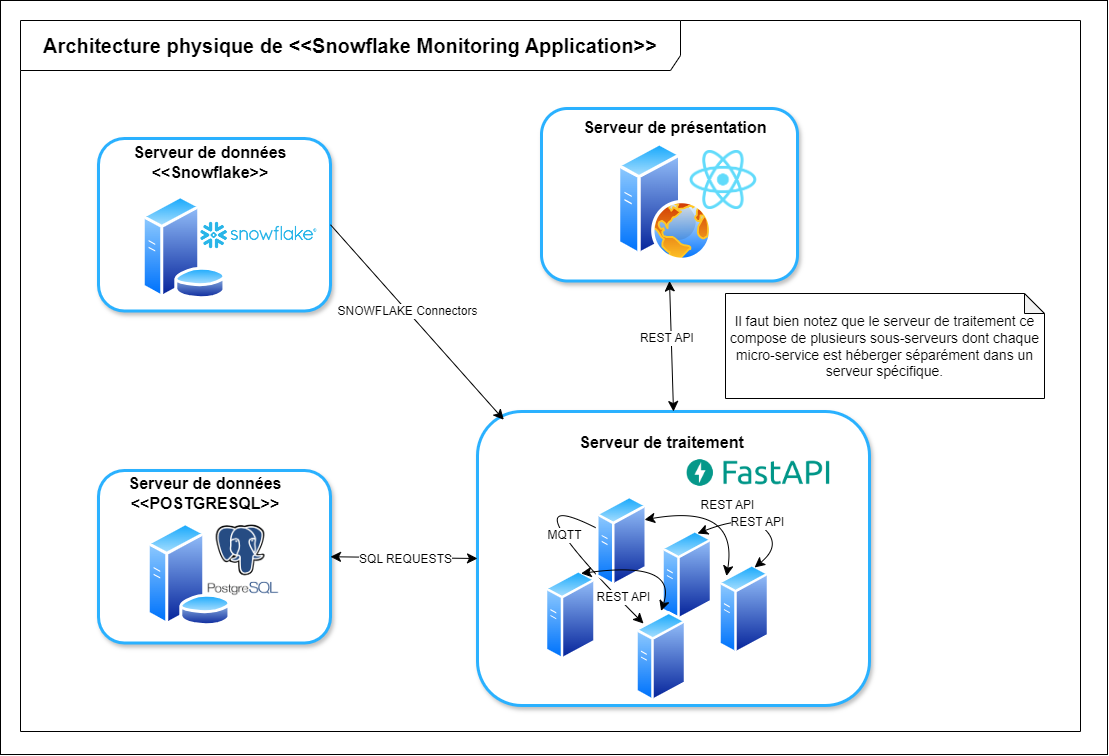
\includegraphics[width = 17cm ]{img/conception/archi_phy.png}
        \caption{Architecture physique de <<Snowflake Monitoring Application>>}
        \label{fig:arch_phy}
        \end{figure}
        %fin
        \par Notre architecture physique est composée de plusieurs éléments essentiels qui travaillent en tandem pour permettre la collecte, le traitement, le stockage et la présentation des données de manière optimale. Voici un aperçu détaillé de ces composants :
        \begin{enumerate}
            \item[1-] \textbf{Tier des Services (Tier Application): } 
            cet tier comprend les différents serveurs d'application hébergeant les microservices du système.
            \par Il inclut des serveurs pour les services DAGS\_MONITOR, WAREHOUSE\_USAGE, QUERY\_PERFORMANCE, ETL\_service, AUTH\_service, etc.
            \par Ces serveurs sont responsables de la logique métier et du traitement des données.
            \item [2-] \textbf{Tier des Données:} 
            cet tier est composé du serveur de base de données hébergeant la base de données MONITORING\_DB.
            \par Il est chargé du stockage et de la gestion des données de monitoring collectées.
            \par Le serveur Snowflake, hébergeant la base de données SNOWFLAKE\_SYSTEM\_DB, fait également partie de ce tier des données.
             
            \item[3-]  \textbf{Tier de présentation: }
            cet tier comprend le serveur frontend hébergeant le service ui\_service (Frontend).
            \par Il est responsable de la présentation des données de monitoring aux utilisateurs via les tableaux de bord et les interfaces.
            \item[4-] \textbf{inter-communication:}
            cet tier représente les modes de communication utilisés entre les composants de l'architecture, via les requêtes SQL, les API REST, les connecteurs Snowflake et le système de messagerie MQTT.

        \end{enumerate}
    \par Cette architecture en n-tiers offre plusieurs avantages clés, tels que la séparation des préoccupations, l'évolutivité, la résilience et la sécurité renforcée du système. 
    Chaque tier étant responsable d'une fonction spécifique, il devient plus aisé de maintenir, de mettre à l'échelle et de sécuriser les différents composants de manière indépendante.
\section{Étude conceptuelle}
\par Dans cette section nous allons s'intéresser à la modélisation de notre projet à l'aide des différents modelés et diagrammes qui vont nous permettre de mieux comprendre le flux de travail ainsi la nature des données et les traitements qui circulent dans notre système.
\subsection{Conception globale}
    \par Dans cette section, nous allons s'intéresser à presenter les differents diagrammes illustant la conception globale de notre solution.
    \subsubsection{Diagramme de paquetages}
    \par Les diagrammes de paquetages sont des diagrammes structurels qui illustrent l'organisation et la disposition de différents éléments modélisés sous forme de packages\cite{diag_pack}.

    \par Il sert à grouper des éléments en un ensemble cohérent, et à fournir un espace de noms pour ces éléments.\par La figure \textbf{\ref{fig:e_a}} qui suit représente le diagramme de paquetages de notre système: 
        %code image
            \begin{figure}[H]
            \centering
            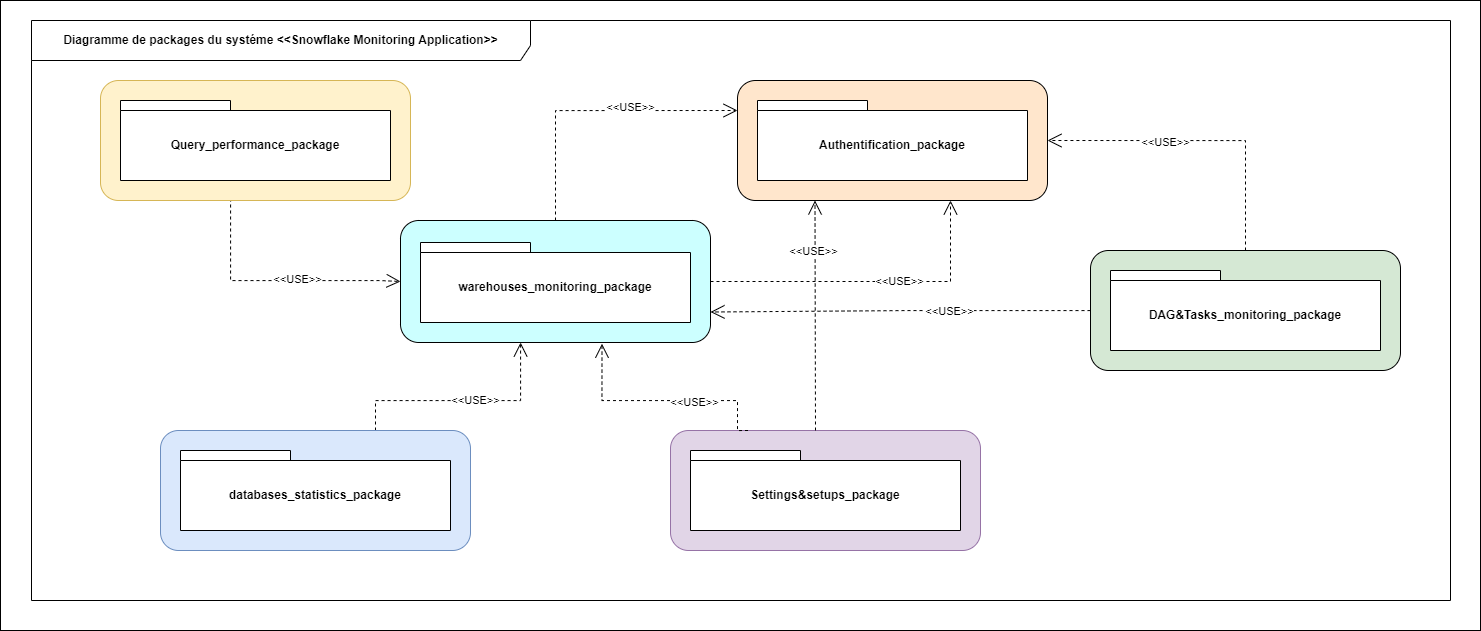
\includegraphics[]{img/conception/diag_pack.png}
            \caption{Diagramme de paquetages de <<Snowflake Monitoring Application>>}
            \label{fig:e_a}
            \end{figure}
        %fin
    \subsubsection{Diagramme de classe}
        \par Les diagrammes de classes fournissent une représentation détaillée de la structure d'un système spécifique.
        Ils modélisent les classes du système, leurs attributs, leurs opérations ainsi que les relations entre les objets\cite{diag_class}. 
        \par Ce diagramme permet de visualiser clairement la composition du système, facilitant ainsi la compréhension des interactions et des dépendances entre les différents éléments. 
        En représentant les attributs et les méthodes des classes, ils aident également à définir les responsabilités et les comportements des objets dans le contexte global du système.
        \par La figure \textbf{\ref{fig:class}} qui suit représente le diagramme de classe de notre système: 
        %code image
        \begin{figure}[H]
            \centering
            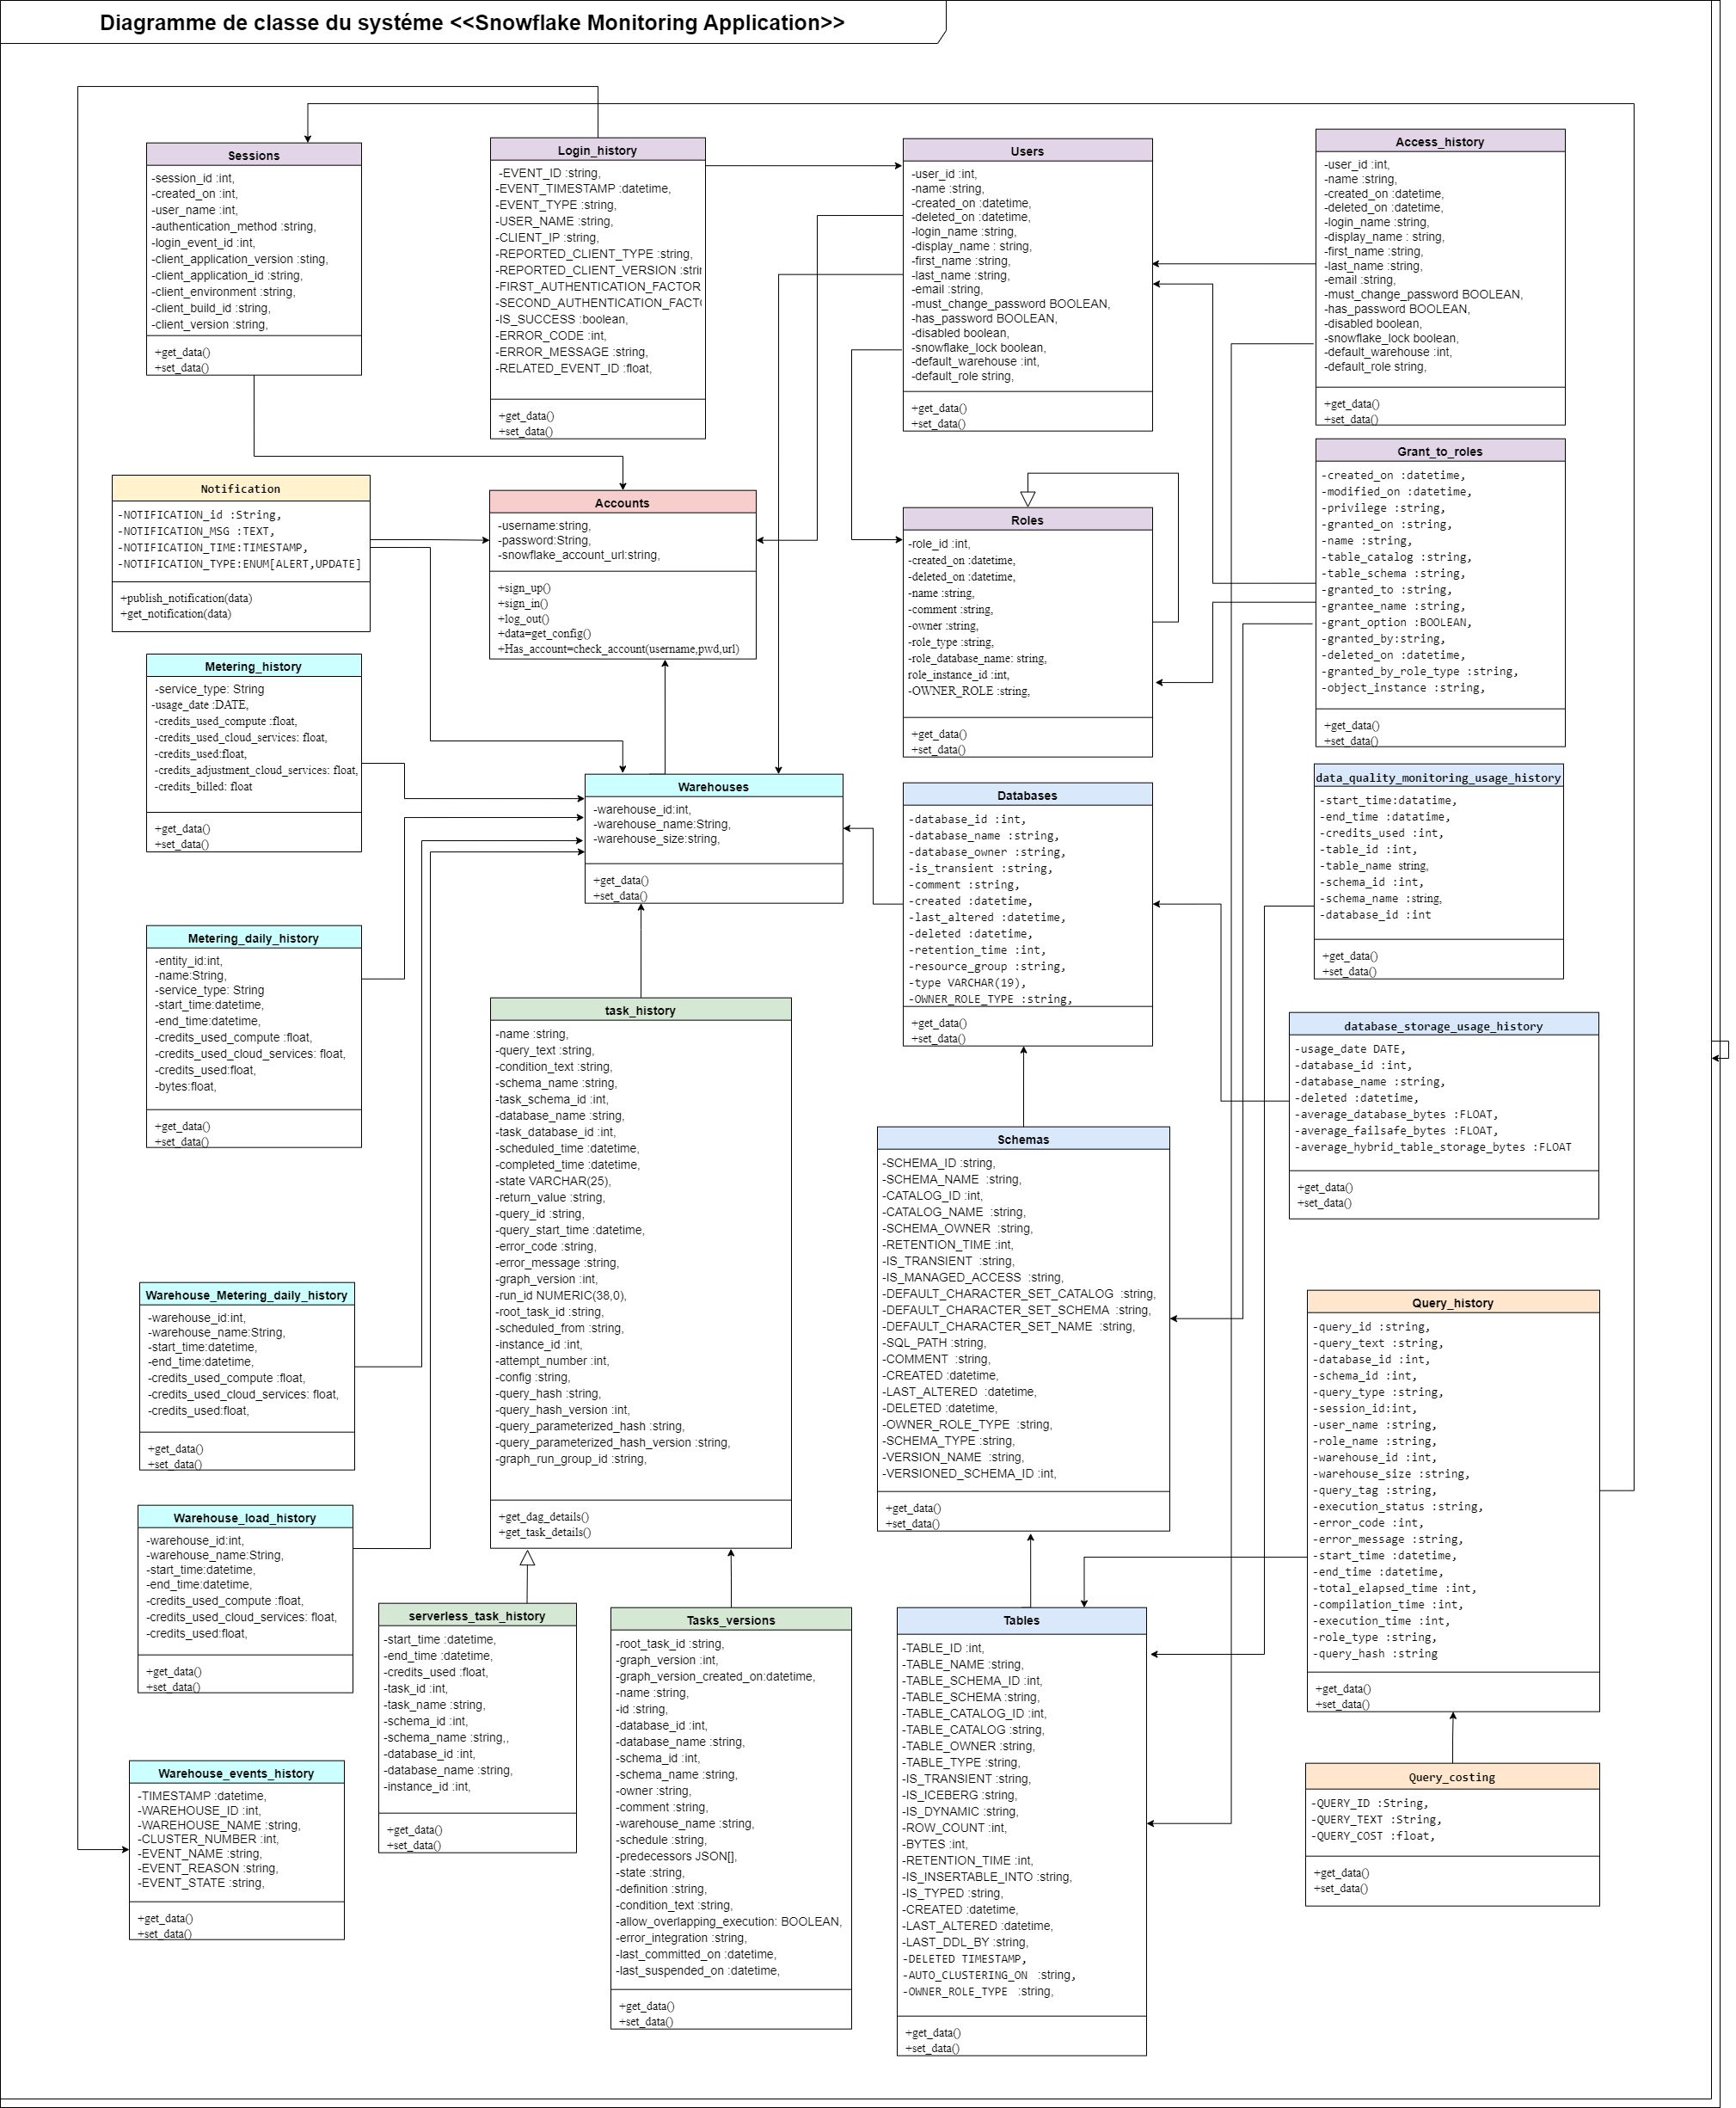
\includegraphics[width =1\linewidth, height=22cm]{img/conception/class.png}
            \caption{Diagramme de classe de <<Snowflake Monitoring Application>>}
            \label{fig:class}
            \end{figure}
        %fin
    \subsubsection{Diagramme de cas d'utilisation global}
    \par Le but fondamental d'un diagramme de cas d'utilisation UML consiste à illustrer les diverses interactions entre un utilisateur et un système \cite{use_case}.
    \par  \par La figure \textbf{\ref{fig:use}} qui suit représente le diagramme de cas d'utilisation global de notre système:     
    %code image
        \begin{figure}[H]
            \centering
            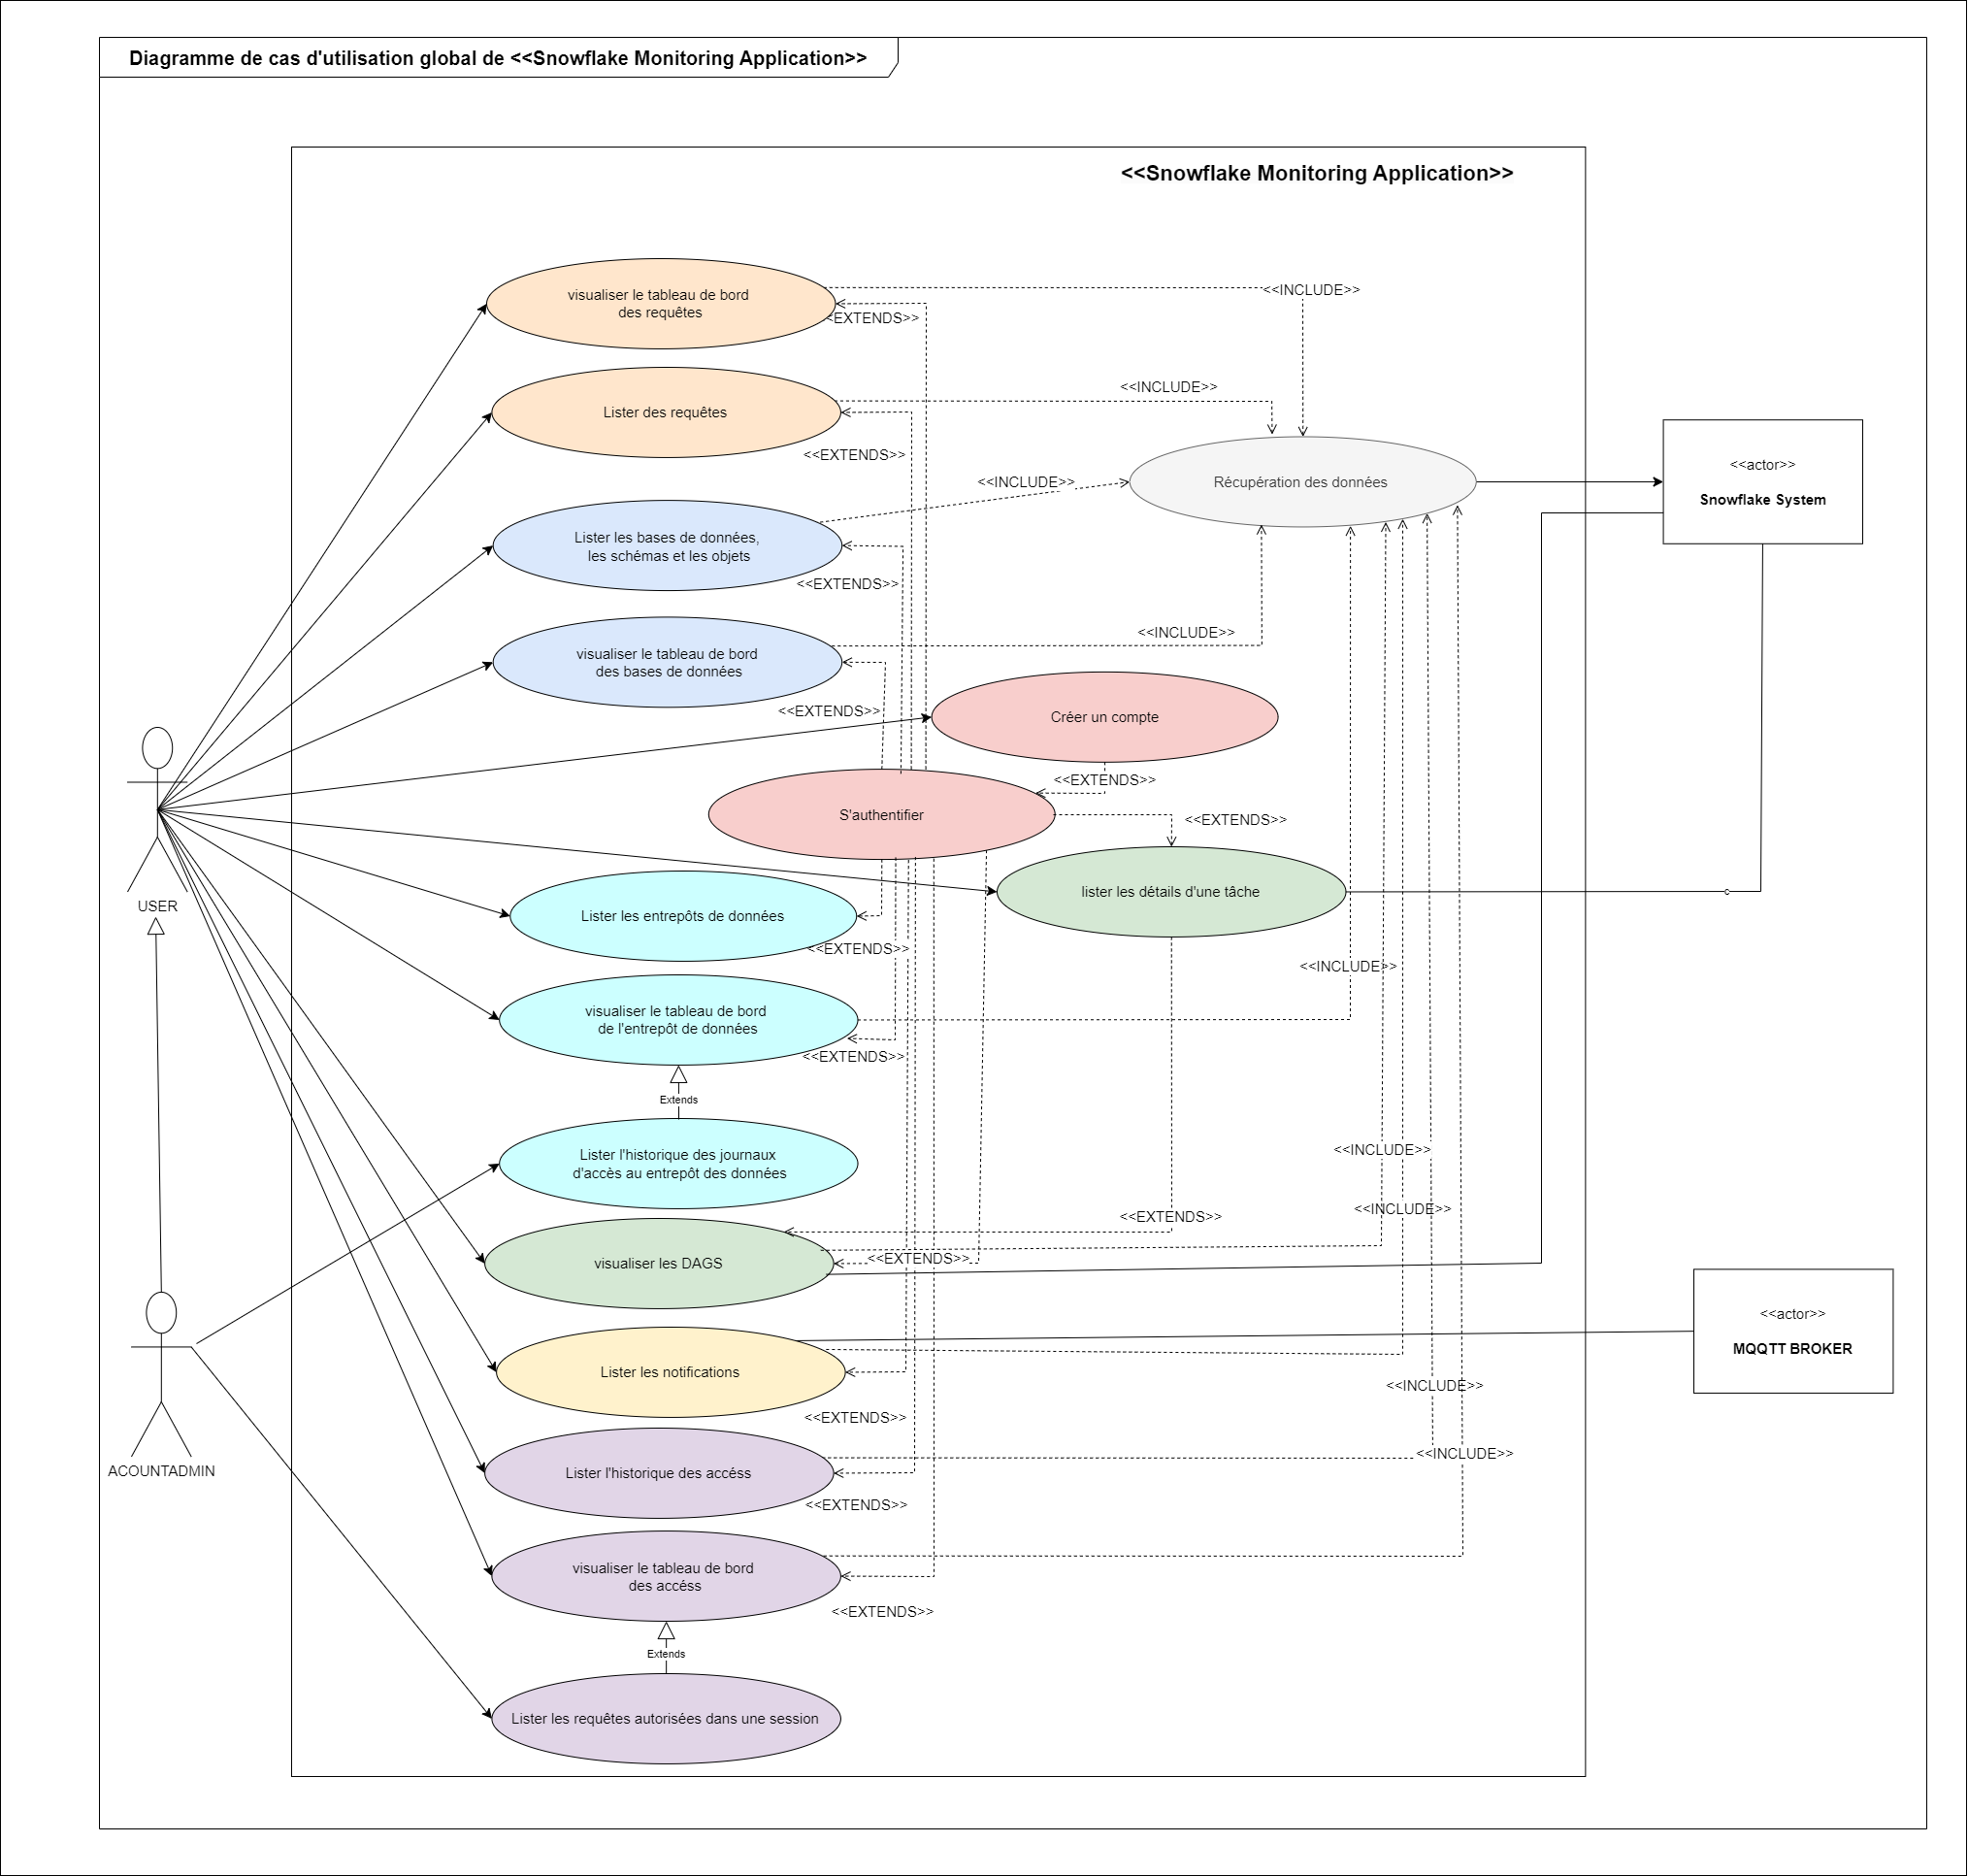
\includegraphics[ height=17cm]{img/conception/use_case.png}
            \caption{Diagramme de cas d'utilisation globale <<Snowflake Monitoring Application>>}
            \label{fig:use}
            \end{figure}
        %fin
\subsection{Conception detaillée}
    \par Dans cette section, nous allons s'intéresser à présenter les diagrammes illustant la conception détaillée de chaque micro-service présent dans solution.
        
\subsubsection{Description textuelle des cas d'utilisation}
\par c'est une description claire et précise des interactions entre les acteurs et le système pour mener à bien le cas d'utilisation. Cette description identifie les acteurs impliqués ainsi que les autres cas d'utilisation pertinents\cite{descp}.
\begin{enumerate}
    \item[1.] \textbf{Description textuelle du cas d'utilisation <<Lister les entrepôts de données>>:}
    \begin{table}[H]
        \centering
            \begin{tabular}{|p{3.5cm}|p{12cm}|}
                \hline \textbf{Titre} &  Lister les entrepôts de données \\
                \hline \textbf{Résumé} & L'utilisateur souhaite de lister les données de ses entrepôts de données' \\
                \hline \textbf{Acteurs} & Utilisateur\\
                \hline \textbf{Pré conditions }& L'utilisateur est authentifié et autorisé, via une token, à accéder à cette fonctionnalité\\
                \hline \textbf{Scénarios Nominaux} &
                    \begin{enumerate}
                        \item [1.] L'utilisateur sélectionne l'option <<Warehouses>>,
                        \item [2.] l'application récupère la liste des entrepôts et leurs données de la base de données Monitoring\_DB,
                        \item [3.] l'application affiche les informations détaillées sur chaque entrepôt (nom, taille, performances, etc.),
                        \item [4.] l'utilisateur peut consulter les détails de chaque entrepôt.      
                    \end{enumerate}\\
                        \hline \textbf{Scénario alternatif} & 
                        3.a. \hspace{0.3cm} [«Pas de warehouses»]: Le système retourne un tableaux indiquant que la liste est vide \newline                             \\
                \hline  \textbf{Scénarios d'exceptions} & 
                    [«Token éxpirée»]: Le système signale l'erreur et redirecte l'utilisateur vers la page de <<login>>.\\
                \hline \textbf{Post conditions} & L'utilisateur a accès à la liste des entrepôts de données et peut consulter leurs informations détaillées.
         \\
                \hline
            \end{tabular}
            \caption{description textuelle de cas d'utilisation <<Lister les entrepôts de données>>}
        \end{table}
        \newpage
        \vspace{2cm}
        \item[2.] \textbf{Description textuelle du cas d'utilisation <<Lister les requêtes SQL>>:}
    \begin{table}[H]
        \centering
            \begin{tabular}{|p{3.5cm}|p{12cm}|}
                \hline \textbf{Titre} &  Lister les requêtes SQL \\
                \hline \textbf{Résumé} & L'utilisateur souhaite de lister les données de ses entrepôts de données' \\
                \hline \textbf{Acteurs} & Utilisateur \\
                \hline \textbf{Pré conditions }& L'utilisateur est authentifié et autorisé, via une token, à accéder à cette fonctionnalité\\
                \hline \textbf{Scénarios Nominaux} &
                    \begin{enumerate}
                        \item [1.] L'utilisateur sélectionne l'option <<<Queries>> ;
                        \item [2.] le système récupère la liste des requêtes SQL exécutées par cet utilisateur de la base de données Monitoring\_DB ;
                        \item [3.] le système affiche les informations détaillées sur chaque requête (ID, type, status, etc.) ;
                        \item [4.] l'utilisateur peut consulter les détails de chaque requête.      
                    \end{enumerate}\\
                        \hline \textbf{Scénario alternatif} & 
                            2.a. \hspace{0.3cm} [«Aucune requête trouvée »]: Le système retourne une liste vide en indiquant qu'il y aucune ligne\\
                \hline  \textbf{Scénarios d'exceptions} & 
                  [«Token éxpirée»]: Le système signale l'erreur et redirecte l'utilisateur vers la page de <<login>>.\\
                \hline \textbf{Post conditions} & L'utilisateur a accès à la liste des entrepôts de données et peut consulter leurs informations détaillées.\\
                \hline 
            \end{tabular}
        \caption{description textuelle de cas d'utilisation <<Lister les requêtes SQL>>}
        \end{table}
        \par \textbf{Il faut mentionner que : } Si l'utilisateur est un \textbf{administrateur} le deuxième point de scénario nominal est modifiée. 
        Car dans ce cas, le systéme va retourner la liste de tout les requêtes SQL exécutées par tout le monde.
\newpage
\vspace{2cm}
        \item[3.] \textbf{Description textuelle du cas d'utilisation <<Lister l'historique des journaux d'accès au entrepôt des données>>:}
    \begin{table}[H]
        \centering
        \begin{tabular}{|p{3.5cm}|p{12cm}|}
            \hline \textbf{Titre} &  Lister l'historique des journaux d'accès au entrepôt des données\\
            \hline \textbf{Résumé} & L'l'administrateur souhaite de lister l'historique des journaux d'accès à un entrepôt des données \\
            \hline \textbf{Acteurs} & Administrateur \\
            \hline \textbf{Pré conditions }& L'administrateur est authentifié et avoir le role autorisé, via une token, à accéder à cette fonctionnalité\\
            \hline \textbf{Scénarios Nominaux} &
                \begin{enumerate}
                    \item [1.] L'administrateur sélectionne l'option <<<warehouse Monitoring>> ;
                    \item [2.] le système récupère les données nécéssaires pour afficher le tableau de bord des entrepôts de donnés  ;
                    \item [3.] l'administrateur sélectionne un entrepôt parmis la liste des entrepôts ;
                    \item [4.] le système renvoi les données spécifiques à cet entrepôt et liste ces journaux d'accées ainsi leurs détails dans le tableau de bord.      
                \end{enumerate}\\
                    \hline \textbf{Scénario alternatif} & 
                    2.a. \hspace{0.3cm} [«Aucun entrepôt trouvé »]: Le système retourne un tableau de bord vide en indiquant qu'il y a pas de données à monitorer.\\
            \hline  \textbf{Scénarios d'exceptions} & 
              [«Token éxpirée»]: Le système signale l'erreur et redirecte l'administrateur vers la page de <<login>>.\\
            \hline \textbf{Post conditions} & L'administrateur a accès à la liste des journaux d'accès au entrepôt des données leurs informations détaillées.\\
            \hline 
        \end{tabular}
        \caption{description textuelle de cas d'utilisation <<Lister l'historique des journaux d'accès au entrepôt des données>>}
        \end{table}
        
        \item[4.] \textbf{Description textuelle du cas d'utilisation <<Lister les bases de données, les schémas et les objets>>:}
    \begin{table}[H]
        \centering
        \begin{tabular}{|p{3.5cm}|p{12cm}|}
            \hline \textbf{Titre} &  Lister les bases de données et leurs objets\\
            \hline \textbf{Résumé} & L'l'utilisateur souhaite de lister les bases de données et leurs objets \\
            \hline \textbf{Acteurs} & utilisateur \\
            \hline \textbf{Pré conditions }& L'utilisateur est authentifié et autorisé, via une token, à accéder à cette fonctionnalité\\
            \hline \textbf{Scénarios Nominaux} &
                \begin{enumerate}
                    \item [1.] L'utilisateur sélectionne l'option <<Databases>> ;
                    \item [2.] le système récupère la liste des bases de données existants dans le compte Snowflake de l'utilisateur en affichant les détailles de chaque base (Id, nom, date de création, etc.) ;
                    \item [3.] l'utilisateur sélectionne une base de données de la liste ;
                    \item [4.] le système récupére l'ID de cette base et lance une recherche dans la base de données Monitoring\_DB des schémas appartenant à cette base ;
                    \item [5.] le systéme affiche la liste des schémas de données de la base sélectionnée avec leurs détailles ;
                    \item [6.] l'utilisateur sélectionne un schéma d'aprés la liste des schémas pour lister les objets conteant dans cet schéma ;
                    \item [7.] le système récupére l'ID de cet schéma et lance une recherche dans la base de données Monitoring\_DB des objets appartenant à ce schéma de données ;
                    \item [8.] le système affiche la liste des objets avec tout les détailles.
                \end{enumerate}\\
                    \hline \textbf{Scénario alternatif} & 
                    2.a. \hspace{0.3cm} [«Aucune base de données trouvée »]: Le système retourne une liste des base de données vide.
                    4.a. \hspace{0.3cm} [«Aucun schéma trouvé »]: Le système retourne une liste des schémas vide.
                    7.a. \hspace{0.3cm} [«Aucun objet trouvé »]: Le système retourne une liste des objets vide.\\
            \hline  \textbf{Scénarios d'exceptions} & 
              [«Token éxpirée»]: Le système signale l'erreur et redirecte l'utilisateur vers la page de <<login>>.\\
            \hline \textbf{Post conditions} & L'utilisateur a accès aux listes des base de données, des schémas et des objets ainsi que leurs informations détaillées.\\
            \hline 
        \end{tabular}
        \caption{description textuelle de cas d'utilisation <<Lister les bases de données, les schémas et les objets>>}
        \end{table}
\end{enumerate}
\subsubsection{Diagrammme d'activité du cas d'utilisation <<Récupération des données >>:}
\par Les diagrammes d'activités démontrent la logique d'un algorithme. De plus, ils fournissent une vue détaillée du comportement d'un système en décrivant la séquence d'actions au sein d'un processus\cite{diag_act}.
\par Le diagramme d'activité du cas d'utilisation ETL-service est représenté dans la figure \textbf{\ref{fig:act}} suivante:
    %code image
    \begin{figure}[H]
        \centering
        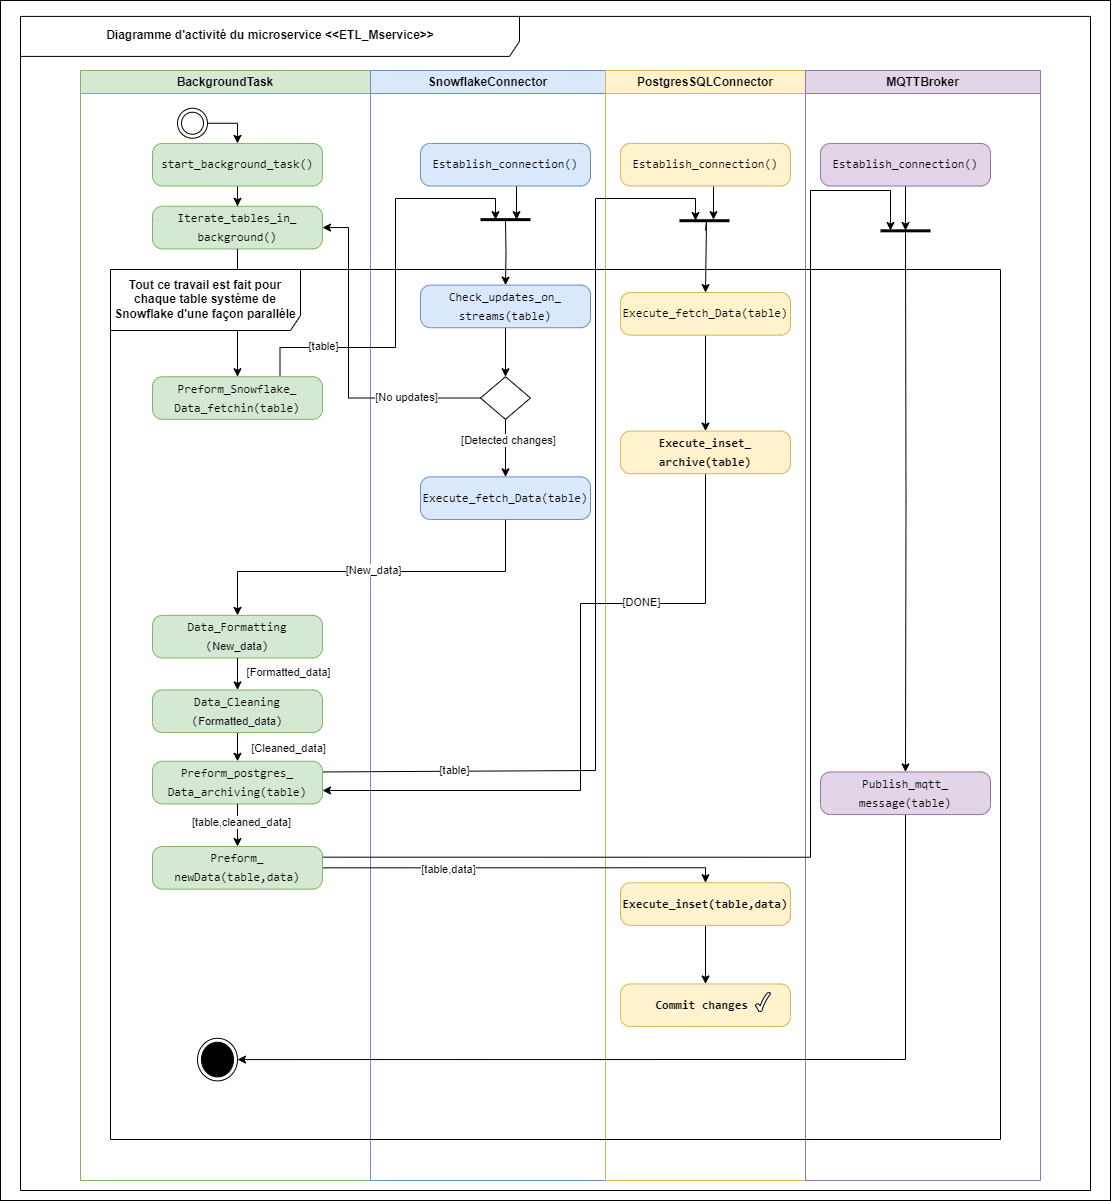
\includegraphics[width=1\linewidth, height=17cm]{img/conception/diag_act_1.png}
        \caption{Diagramme d'activité du cas d'utilisation <<Récupération des données >>}
            \label{fig:act}
        \end{figure}
    %fin
\par Le traitement du cas d'utilisation <<Récupération des données >> commence par l'appele la méthode \textbf{<<start\_background\_task()>>}, qui est une méthode programmée automatiquement chaque 24 heurs.
En lancant cette méthode, elle parcourt les tables du système Snowflake, dont nous voulons projeter, en utilisant la méthode \textbf{<<iterate\_tables\_in\_background()>>}.
\par À ce stade, le connecteur Snowflake établit une connexion avec le système Snowflake via la méthode \textbf{<<establish\_connection()>>}, 
qui à ca part connecte notre service avec le compte Snowflake dont nous souhaitons monitorer ces données plus tard.
\par Ensuite, le contrôleur système vérifie s'il y a des mises à jour sur les tables Snowflake en appelant la méthode \textbf{<<check\_updates\_on\_streams(tables)>>}. 
\par Si il y des changements détectés, la méthode \textbf{<<execute\_fetch\_data(table)>>} est exécutée pour récupérer les nouvelles données de la table Snowflake.
\par Les nouvelles données récupérées sont ensuite transmises à l'étape de formatage des données \newline \textbf{<<Data\_Formatting()>>}, où elles sont mises en forme(typage, longeur, format etc.). 
Après cela, l'étape de nettoyage des données \textbf{<<Data\_Cleaning()>>} intervient pour préparer et nettoyer les données formatées. 
\par Postérieurement, l'étape d'archivage des données dans PostgreSQL \textbf{<<Preform\_Data\_archiving>>}, là où nous allons transformer les anciennes données de cette table vers une base de données d'archivage afin d'avoir toujours une traçabilité des données. 
\par Parallèlement, le connecteur PostgreSQL établit une connexion avec les base de données PostgreSQL, \textbf{monitoring\_db} et la base d'archive \textbf{backup\_db}, via la méthode \textbf{<<establish\_connection()>>}. 
tout en éxécutant la méthode \textbf{<<execute\_insert\_archive(table, data)>>}. 
\par Par la suite,le système déclanche la methode \textbf{<<Preform\_newData(table,data)>>} pour insérer les nouveaux données nettoyées dans la base de données de monitoring. 
Après l'insertion des données, le microservice effectue un commit des changements dans la base de données.
\par il faut notez bien que, ce flux de travail ce repéte éventuellement pour chaque table, séparament ou/et séquentiellement pour les tables qui on une relation entre eux, dans un \textbf{<<thread>>} à part.
\par Aprés la mise à jour de tout les tables, il publie un message MQTT via la méthode \newline \textbf{<<publish\_mqtt\_message()>>} afin de notifier le systéme de l'ajout de nouvelles données. 
\par Cette approche garantit que toutes les étapes sont correctement coordonnées et que chaque composant est informé des mises à jour de manière efficace et en temps réel.
\par Enfin, le microservice ETL-service termine son traitement en attendant son prochain déclanchement.
\subsubsection{Diagrammme de séquence de cas d'utilisation <<Visualiser DAG>>:}
\par Les diagrammes d'activités démontrent la logique d'un algorithme. De plus, ils fournissent une vue détaillée du comportement d'un système en décrivant la séquence d'actions au sein d'un processus\cite{diag_act}.
\par Le diagramme de séquence de cas d'utilisation <<Visualiser DAG>> est représenté dans la figure \textbf{\ref{fig:seq1}} suivante:
    %code image
    \begin{figure}[H]
        \centering
        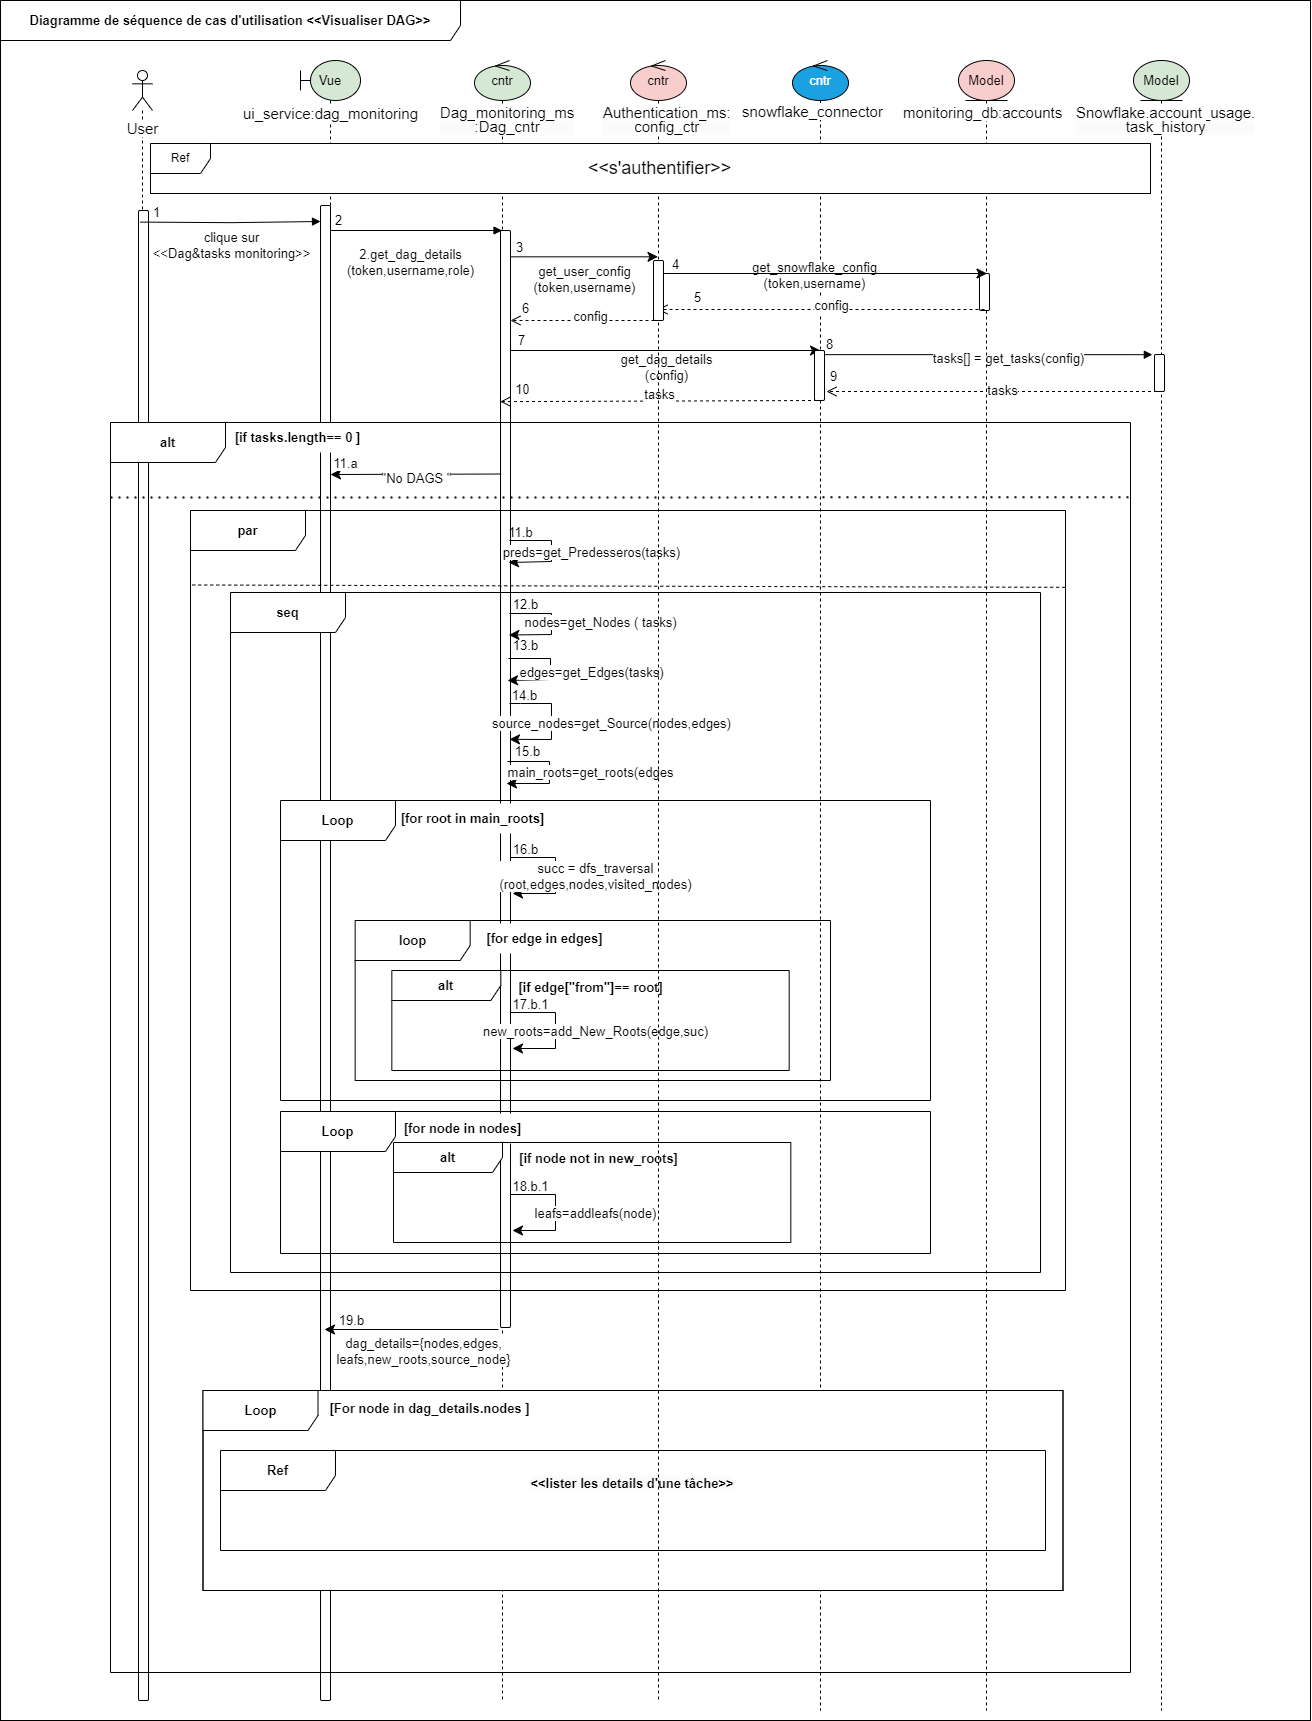
\includegraphics[width =1\linewidth, height=23.5cm]{img/conception/seq1.png}
        \caption{Diagrammme de séquence de cas d'utilisation <<Visualiser DAG>> }
            \label{fig:seq1}
    \end{figure}
    \par Ce diagramme de séquence décrit le cas d'utilisation \textbf{<<Visualiser le DAG>>} où 
    un utilisateur souhaite visualiser les détails du Directed Acyclic Graph (DAG) des tâches Snowflake en temps réel.
    \par Le traitement ce lance lorsque l'utilisateur clique sur le bouton <<Task\&Dag Monitoring>> de l'interface, 
    cette action lance un appel au contrôleur du micro service <<DAG\_monitoring>> pour récupérer les DAGs.
    Une fois l'appel est lancé, le contrôleur en question envoit à son tour une requête au micro-service d'authentification pour avoir les configurations de compte Snowflake assosiés au nom d'utilisateur avec la token d'autorization.
    \par Le contrôleur snowflake config\_ctr du service d'authentification renvoit les configurations néssesaires au contrôleur principal.
    \par Une fois les configurations sont retournées, le contrôleur de DAG\_monitoring fait appel au snowflake\_connector, qui est le point de communication direct entre l'application et Snowflake, pour accéder au compte Snowflake de l'utilisateur et récupérer la liste des tâches qui lui sont associées.
    \par le contrôleur snowflake\_ctr effectue les opérations nécessaires sur Snowflake et retourne la liste des tâches au DAG\_ctr:
    \begin{itemize}
        \item \textbf{Si [la longeur de la liste égal à 0];} le contrôleur DAG\_ctr renvoit un message au service du frontend en indiquant qu'il y a aucune DAG pour cette utilisateur,
        \item \textbf{Sinon;} \parindent=1.5em \par -le contrôleur DAG\_ctr commance le traitement sur les tâches retournées, en récupérant la liste des prédécesseurs de chaque tâches.
       
        \parindent=1.5em \par -Parallèlement, dans un autre thread séparament, il recupére:les noeuds (nodes), les arêtes (edges), les noeuds sources (source\_nodes), les routes principales (main\_roots). 
        \parindent=1.5em \par -Ensuite, pour chaque route il fait un parcours en profondeur (DFS\_transfersal) afin marquer les noeuds visités et collecter les successeurs. 
        \parindent=1.5em \par -Puis, il verife pour chaque arête, si l'arête part de la racine actuelle et si c'est le cas, il ajoute le noeud de destination au new\_roots qui sera l'ensemble des nouvelles racines pour la prochaine itération de la boucle principale.
        \parindent=1.5em \par -Aprés tout cela, il parcourt tout les noeuds pour identifier les noeuds feuilles, ceux qui ne sont pas dans new\_root.
        \parindent=1.5em \par -Finalement, il renvoit tout les informations traitées aux service frontend comme etant un objet JSON.
                
    \end{itemize}
    \par Enfin, le service frontend va lui même parcourue les noeudes de l'objet retourné, en dessinant le DAG finale en faisant appel au contrôleur Task\_details (cas d'utilisation <<lister les details d'une tâche>>) inclus du même service pour afficher en details chaque noeud du DAG.
    \par \textbf{NB:} Il faut bien préciser que le declanchement de cet cas d'utilisation nécessite l'authentification de l'utilisateur et qu'il a les permissons et les roles qui lui permet de visualiser les DAG.
    \subsubsection{Diagramme de séquence du cas d'utilisation <<Lister les détaills d'une tâche>>:}
    \par La figure \textbf{\ref*{fig:seq2}} illustre le diagramme de séquence du cas d'utilisation <<Lister les détaills d'une tâche>>:

    \begin{figure}[H]
        \centering
        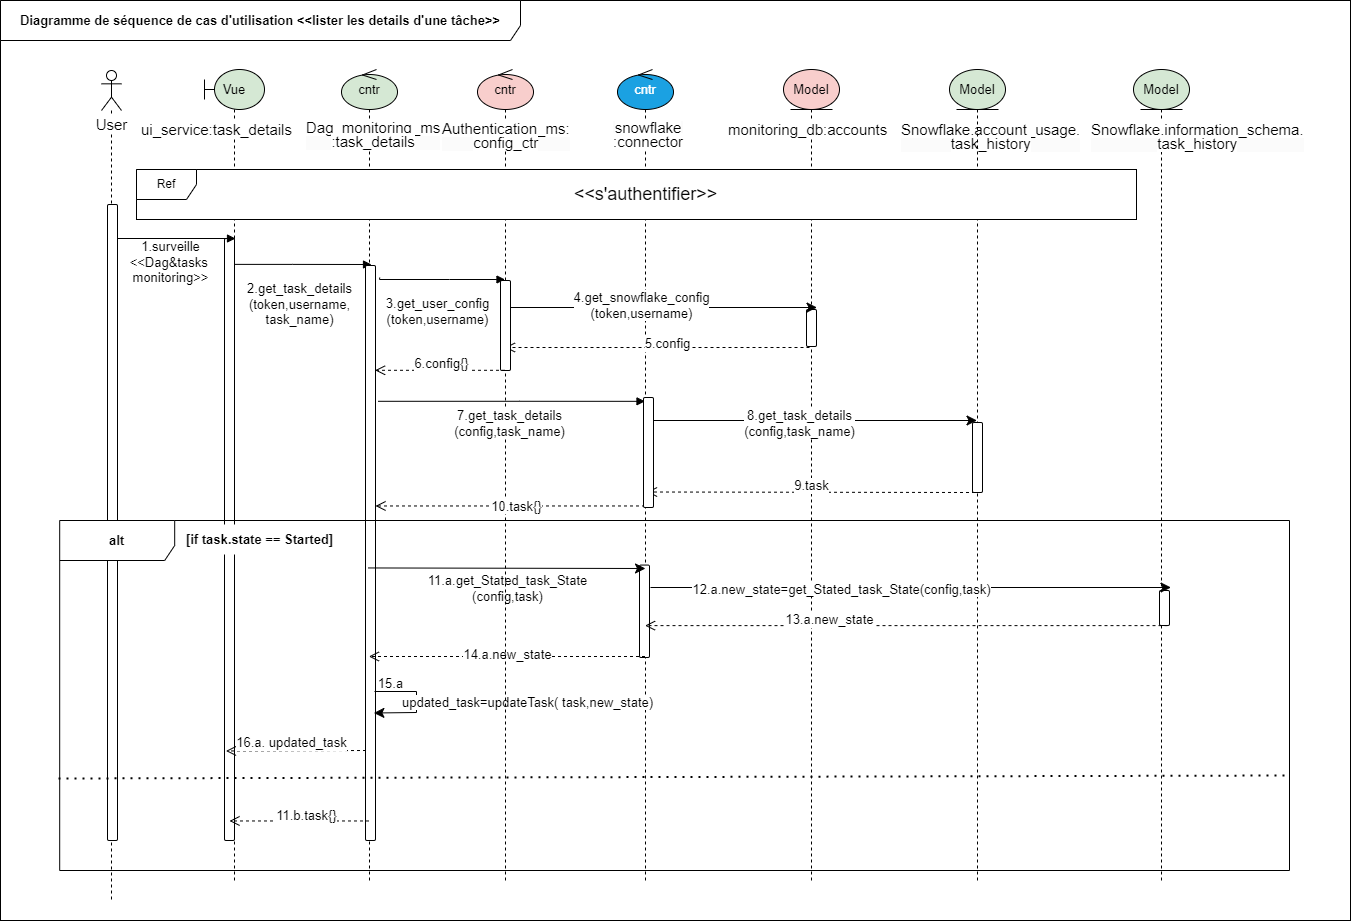
\includegraphics[width=1\linewidth ,height=17cm]{img/conception/seq2.png}
        \caption{Diagrammme de séquence de cas d'utilisation <<Lister les détaills d'une tâche>> }
        \label{fig:seq2}
    \end{figure}
    \par Pour Lister les details d'une tâche, et aprés avoir vérifier que l'utilisateur est authentifié, le service du frontend lance un appel au contrôleur task\_details 
    pour récupérer les données souhaitées. 
    \par En lançant cet contrôleur, il envoit à son tour une requête au micro-service d'authentification pour avoir les configurations de compte Snowflake assosiés au nom d'utilisateur avec la token d'autorization.
    \par Le contrôleur snowflake config\_ctr du service d'authentification renvoit les configurations néssesaires au contrôleur principal.
    \par Une fois les configurations sont retournées, le contrôleur de DAG\_monitoring fait appel au \par snowflake\_connector, qui est le point de communication direct entre l'application et Snowflake, 
    pour accéder au compte Snowflake de l'utilisateur et récupérer les détailles de tâche en question de la vue \textbf{Task\_History} du schéma système de snowflake \textbf{Account\_Ussage}, qui a des informations global sur les tâches.
    \par le contrôleur snowflake\_ctr effectue les opérations nécessaires sur Snowflake et retourne les détailles du task demandé sous le format JSON.
    \par Le contrôleur task\_details traite le résultat retourné; 
    \begin{itemize}
        \item \textbf{Si [L'état du tâche est <<Started>>]:} 
        \par - le contrôleur task\_details relance un autre appel au snowflake\_connector,
        \par - ce dernier il va accéder à nouveau à Snowflake mais cette fois si il va opérer la vue \textbf{Task\_History} du schéma \textbf{Information\_schema} de Snowflake, qui est la vue qui a les informations sur les tâches commencées, pour récupérer l'êtat de cette tâche en temps rélle qui peut être ( plannifiée, entrain de s'éxécuter ou échouée),
        \par - une fois le nouveau état est retourner task\_details met à jour les données en modifiant l'état <<Started>> par le nouveau ètat du tâche et l'envoyer au service du frontend en fomat JSON.
        \item \textbf{Sinon [L'état sera <<suspended>>]:} le controleur va retourner directement les données du tâche au service de frontend sans faire aucune modification.
    \end{itemize}

    \subsubsection{Diagramme de séquence du cas d'utilisation <<Créer un compte>>:}
    \par La figure \textbf{\ref*{fig:seq3}} illustre le diagramme de séquence du cas d'utilisation <<Créer un compte>>:
    \begin{figure}[H]
        \centering
        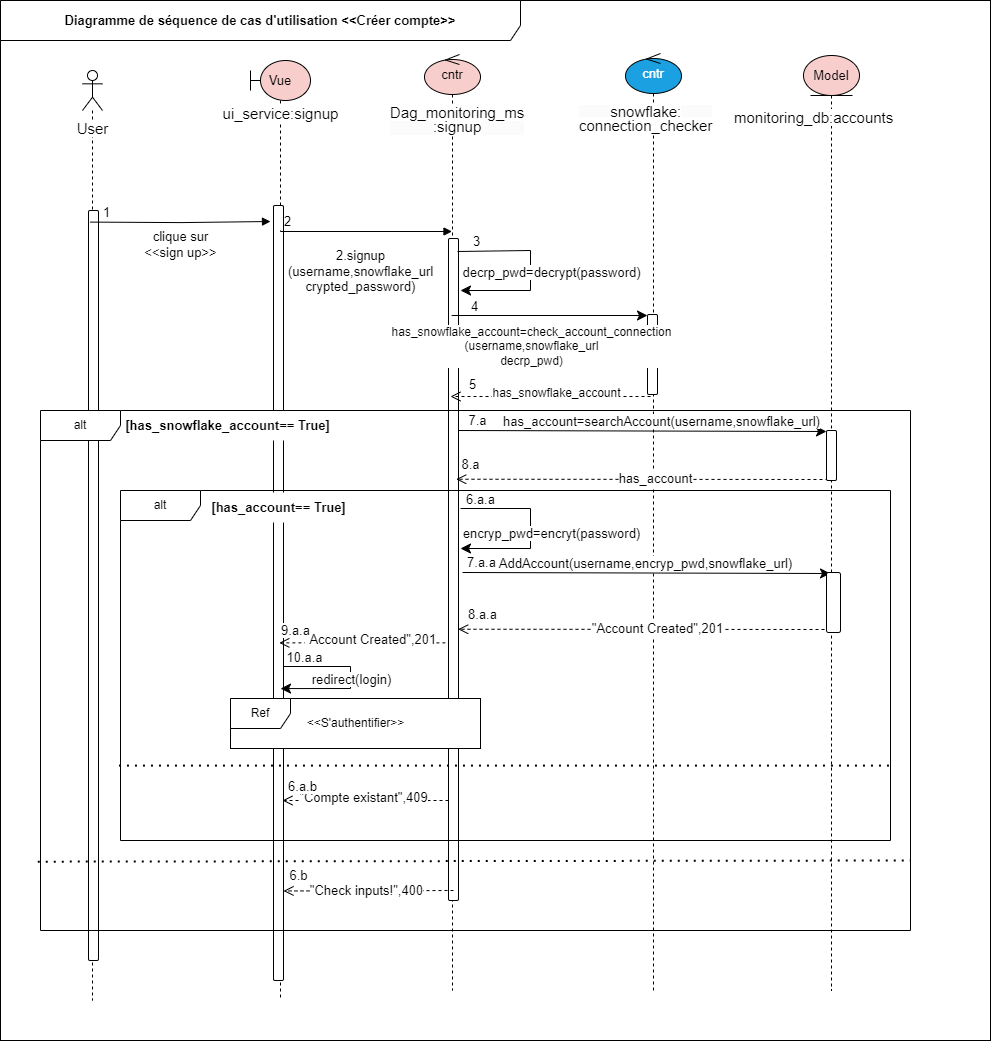
\includegraphics[height=17cm]{img/conception/signup.png}
        \caption{Diagrammme de séquence de cas d'utilisation <<Créer un compte>> }
        \label{fig:seq3}
    \end{figure}
    \par Afin de pouvoir inscrire dans <<Snowflake Monitoring Application>>, l'utilisateur accéde à l'interface de creation de compte de l'application en saisisant son username, mot de passe, 
    ainsi que l'URL d'accés à son compte Snowflake.
    \par En cliquant sur <<signup>>, le contrôleur signup\_ctr récupére les données saisites du frontend et décrypte le mot de passe.
    \par Ensuite, il emettre un appel au contrôleur de snowflake pour que ce dernier vérifie l'existance de ce compte dans Snowflake en retournant une réponse vers le contrôleur principal. 
    \begin{itemize}
        \item \textbf{[has\_snowflake\_account == True]}:
       \par -le contrôleur lance une recherche dans la table de monitoring\_DB \textbf{accounts}
       \par -\textbf{si [has\_account == True]}, le contrôleur renvoit une erreur au frontend.
       \par -\textbf{sinon}, le contrôleur va encrypter le mot de passe et crée un compte dans la table \textbf{accounts} avec les données saisies.
       \par Enfin, il va renvoyer un message de succéss au frontend qui va à son tour rediger l'utilisateur vers la page de l'authentification. 
       \item \textbf{[Sinon]}: 
       \par -Le contrôleur renvoit un message d'erreur au frontend en indiquant que les données saisites n'appartient à aucun compte Snowflake.
    \end{itemize}
    \subsubsection{Diagramme de séquence du cas d'utilisation <<S'authentifier>>:}
    \par La figure \textbf{\ref*{fig:seq4}} illustre le diagramme de séquence du cas d'utilisation <<S'authentifier>>:

    \begin{figure}[H]
        \centering
        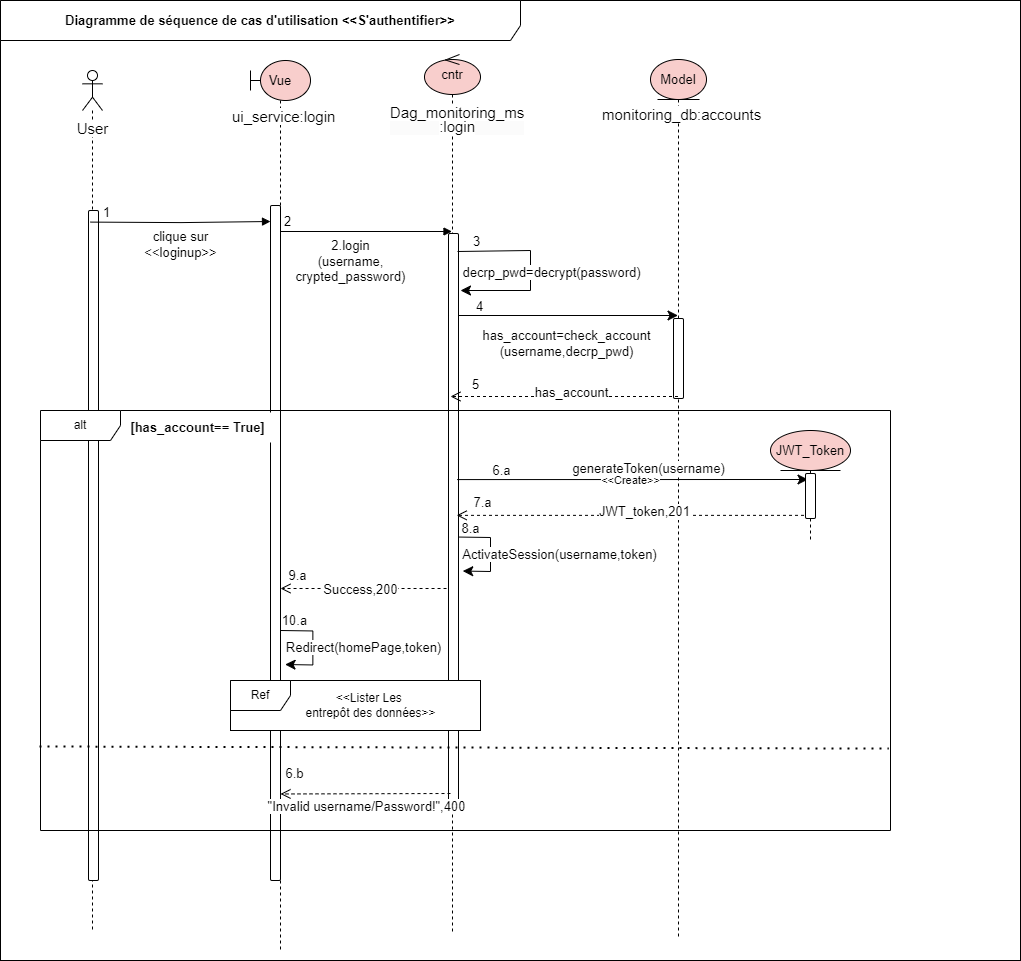
\includegraphics[ height=12cm]{img/conception/login.png}
        \caption{Diagrammme de séquence de cas d'utilisation <<S'authentifier>> }
        \label{fig:seq4}
    \end{figure}
    \par Pour accéder à l'application, l'utilisateur accéde à l'interface de <<login>> en saisisant les données d'authentification (username,mot de passe).
    \par En cliquant sur <<login>>, le contrôleur login\_ctr récupére les données saisies du frontend et décrypte le mot de passe saisie. 
    \par Ensuite, il lance une recherche dans la table \textbf{Accounts} pour vérifier l'existance du compte; 
    \begin{itemize}
        \item \textbf{[Has\_account == True]}: cela signifie que le compte existe déjà, et là le contrôleur crée une instance de l'objet \textbf{JWT Token}, qui est le moyen d'accés à toutes les informations et parties de l'application.
         Une fois l'instance est crée et retourné le contrôleur active la session de connexion de l'utilisateur et retourne la token ainsi que un message de succés au frontend.
        \par Finalement, le frontend redirige l'utilisateur vers la page d'acceuil de l'application.
        \item \textbf{[Sinon (compte inexistant)]}: le contrôleur renvoit un message d'erreur vers le frontend en indiquant que les données saisites sont invalides.
    \end{itemize}
    \section*{Conclusion}
\addcontentsline{toc}{section}{Conclusion }
\par Ce chapitre a établi les bases pour la mise en œuvre technique de notre projet. Les choix architecturaux et conceptuels s'avèrent essentiels pour assurer la stabilité et la performance de notre solution. Dans le prochain chapitre, nous plongerons dans la réalisation concrète de notre projet.
        \clearpage
        
        \chapter{Réalisation}
	
\section*{Introduction}
\addcontentsline{toc}{section}{Introduction }
    Le quatrième chapitre se consacre à la mise en œuvre concrète du projet. Nous explorons les choix techniques que nous avons adoptés et détaillons le travail effectué pour donner vie à notre solution.

\section{Choix technologiques}
\par  Dans cette partie, nous explorerons les décisions stratégiques que nous avons prises concernant les technologies et les outils que nous avons choisis pour la réalisation de notre solution.     
\subsection {Frameworks}   
    \begin{itemize}
        \item \textbf{FastAPI: }
        %code image
        \begin{figure}[!htb]\centering
            \begin{minipage}{0.30\textwidth}
            \centering
              {
\includegraphics[width = 2cm , height=2cm]{img/techno/fast.png}}
              \caption{ \\ FastAPI logo \cite{fastapi}}\label{Fig:Data1}
            \end{minipage}
            \begin {minipage}{0.60\textwidth}
            \par FastAPI est un framework web moderne et rapide (à haute performance) pour la création d'API avec Python,
            basé sur les annotations de type standard de Python\cite{fastapi}. \\
            \par Dans la réalisation de ce projet, nous avons opté pour le choix de FastApi comme notre backend framework vue ces performances extrêmement élevées, comparables à celles de NodeJS et Go, grâce à l'utilisation de Starlette et Pydantic.
            FastAPI est l'un des frameworks Python les plus rapides.\\
            \par Sa Robustesse aussi, car il permet de produire un code prêt pour la production avec une documentation interactive et automatique.
            
            \end{minipage}
        \end{figure}
        %fin
        \item \textbf{React: }
            %code image
            \begin{figure}[!htb]\centering
                \begin{minipage}{0.30\textwidth}
                \centering
                {
\includegraphics[width = 2cm , height=2cm]{img/techno/react.png}}
                \caption{\\ React logo \cite{react}}\label{Fig:Data1}
                \end{minipage}
                \begin{minipage}{0.60\textwidth}
                    \par React est une bibliothèque JavaScript destinée à la création d'interfaces utilisateur (UI) \cite{react}. \\
                    \par Dans la réalisation de ce projet, nous avons opté pour React comme étant notre frontend framework car il  permet de créer des interfaces utilisateur dynamiques et réactives avec une efficacité accrue grâce à sa gestion intelligente des mises à jour via le DOM virtuel.
                \end{minipage}

            \end{figure}
        %fin
    \end{itemize}
    \subsection {Bases de données}
    \newpage
    \begin{itemize}
        \item \textbf{PostgreSQL: }
    
        %code image
        \begin{figure}[!htb]\centering
           \begin{minipage}{0.30\textwidth}
           \centering
             {
\includegraphics[width = 3cm , height=3cm]{img/techno/postgresql.png}}
             \caption{ \\ PostgreSQL logo \cite{pg}}\label{Fig:Data2}
           \end{minipage}
           \begin {minipage}{0.60\textwidth}
           \par PostgreSQL est un puissant système de base de données relationnelle objet open source, développé activement depuis plus de 35 ans, qui lui a valu une solide réputation en termes de fiabilité, de robustesse des fonctionnalités et de performances\cite{pg}. \\
           \par Dans la réalisation de ce projet, nous avons opté pour le choix de PostgreSQL comme étant notre SGBD vue qu'il est est souvent perçu comme un système plus fiable et plus robuste que MySQL pour gérer de grands volumes de données sans risque de corruption.\\
           \par De plus, il permet de stocker des informations de manière plus structurée grâce à une meilleure gestion des relations et des contraintes.
           \end{minipage}
       \end{figure}
    
\end{itemize}
\subsection{Outils de communication}
\begin{itemize}

    \item \textbf{MQTT: }
        %code image
            \begin{figure}[!htb]\centering
            \begin{minipage}{0.30\textwidth}
            \centering
                {
\includegraphics[width = 2cm , height=2cm]{img/techno/mqtt.png}}
                \caption{\\ MQTT logo \cite{mqtt}}\label{Fig:Data1}
            \end{minipage}
            \begin{minipage}{0.60\textwidth}
                \par MQTT est un protocole de messagerie basé sur des normes, ou un ensemble de règles, utilisé pour la communication de machine à machine \cite{mqtt}. \\
                \par Dans la réalisation de ce projet, nous avons opté pour MQTT comme étant un systéme de notification car il MQTT facilite le chiffrement des messages 
                via TLS et l'authentification des clients à l'aide de protocoles d'authentification modernes, tels que OAuth. \\
                \par De plus, sa Légèreté et efficacité car les clients MQTT sont très petits, ils nécessitent peu de ressources. Les en-têtes des messages MQTT sont de petite taille afin d'optimiser la bande passante du réseau.
            \end{minipage}
    \end{figure}
    \item\textbf{RESTful APIs:}
    %code image 
     \begin{figure}[!htb]\centering
        \begin{minipage}{0.30\textwidth}
        \centering
            {
\includegraphics[width = 2cm , height=2cm]{img/techno/rest.png}}
            \caption{\\ REST logo \cite{rest}}\label{Fig:Data1}
        \end{minipage}
        \begin{minipage}{0.60\textwidth}
            \par REST (REpresentational State Transfer) constitue un style architectural et un mode de communication fréquemment utilisé dans le développement de services Web \cite{rest}. \\
            \par Dans la réalisation de ce projet, nous avons opté pour RESTful API comme étant le mode de communiction entre les différents microservices du systéme car ils sont faciles à utiliser avec la plupart des outils. 
            \par De plus REST s'impose progressivement comme le standard pour l'interaction entre systèmes. 
          
        \end{minipage}
    \end{figure}

    \end{itemize}

    \subsection{Bibliothèques pour l'analyse et la manipulation des données}
    \begin{itemize}
        \item \textbf{Snowflake-connector-python: }
       
        %code image 
         \begin{figure}[!htb]\centering
             \begin{minipage}{0.30\textwidth}
             \centering
                 {
\includegraphics[width = 2cm , height=2cm]{img/techno/snowflake.png}}
                 \caption{\\ Snowflake logo \cite{sncn}}\label{Fig:Data1}
             \end{minipage}
             \begin{minipage}{0.60\textwidth}
                 \par Le connecteur Snowflake pour Python fournit une interface pour le développement d'applications Python
                  qui peuvent se connecter à Snowflake et effectuer toutes les opérations standard.\cite{sncn}. \\
                 \par Il a été conçu pour pour gérer les ressources principales de Snowflake, y compris les bases de données, les schémas, les tables, les tâches et les entrepôts, sans utiliser le langage SQL.
        
             \end{minipage}
         \end{figure}
    \item \textbf{psycopg: }
       
       %code image 
        \begin{figure}[!htb]\centering
            \begin{minipage}{0.30\textwidth}
            \centering
                {
\includegraphics[width = 2cm , height=2cm]{img/techno/psycopg.png}}
                \caption{\\ Psycopg logo \cite{psycopg}}\label{Fig:Data1}
            \end{minipage}
            \begin{minipage}{0.60\textwidth}
                \par Psycopg est l'adaptateur de base de données PostgreSQL le plus populaire pour le langage de programmation Python. 
                Il est écrit en C et fournit un moyen d'effectuer toute la gamme des opérations SQL sur les bases de données PostgreSQL\cite{psycopg}. \\
                \par Il a été conçu pour les applications fortement multithreadées qui créent et détruisent de nombreux curseurs et effectuent un grand nombre d'« INSERT “s ou d” »UPDATE « s simultanés. C'est le principal raison pour lequel nous avons choisi cet librairie pour toute interaction avec postgresql.
            
            \end{minipage}
        \end{figure}
        %fin

    \item \textbf{Pandas: }
       
             %code image
             \begin{figure}[!htb]\centering
                \begin{minipage}{0.30\textwidth}
                \centering
                    {
\includegraphics[width = 2cm , height=2cm]{img/techno/pandas.png}}
                    \caption{\\ Pandas logo \cite{pandas}}\label{Fig:Data1}
                \end{minipage}
                \begin{minipage}{0.60\textwidth}
                    \par  Pandas est une bibliothèque de manipulation de données Python qui fournit des structures de données flexibles pour l'analyse des données\cite{pandas}. \\
                    \par Il a été conçu pour facilite l'importation, la manipulation et l'analyse des données, ce qui en fait un choix idéal pour notre projet.
                
                \end{minipage}
            \end{figure}
        %fin
    \item \textbf{GMQTT: }
       
        \par Gmqtt est une bibliothèque de broker MQTT flexible et performante qui implémente entièrement le protocole MQTT V3.x et V5 en golang \cite{gmqtt}. 
   %fin
       
   \end{itemize}
\subsection{Bibliothèques d'interaction avec le système d'exploitation}
\begin{itemize}
    \item \textbf{OS: }
        \par Un module intégré à Python qui permet d'interagir avec le système d'exploitation sous-jacent sur lequel Python est exécuté. 
        Il peut être utilisé pour manipuler le système de fichiers, gérer les variables d'environnement, contrôler les processus, et bien plus encore\cite{os}.

    \item \textbf{Scheduler: }
        \par C'est une bibliothèque simple d'ordonnancement en python avec asyncio, threading ainsi que la prise en charge des fuseaux horaires.\\
         Elle permet de planifiez des tâches en fonction de leurs cycles temporels, d'heures fixes, de jours de la semaine,
         de dates, de poids, de décalages et de comptes d'exécution, et automatisez les tâches\cite{scheduler}.
    \item \textbf{Requests: }
        \par est un standard Python permettant d'effectuer des requêtes HTTP.
         Elle dissimule les subtilités des requêtes derrière une API simple, ce qui vous permet de vous concentrer sur l'interaction avec les services et la consommation de données dans votre application\cite{requests}.
    
\end{itemize}
\subsection{Outils de test}
\begin{itemize}

    \item \textbf{Postman: }
        %code image
            \begin{figure}[!htb]\centering
            \begin{minipage}{0.30\textwidth}
            \centering
                {
\includegraphics[width = 2cm , height=2cm]{img/techno/postman.png}}
                \caption{\\ Postman logo \cite{postman}}\label{Fig:Data1}
            \end{minipage}
            \begin{minipage}{0.60\textwidth}
                \par  Postman agit en tant que client et constitue un excellent outil pour tester des API RESTful. Il offre une interface utilisateur élégante pour effectuer des requêtes HTTP,
                 sans avoir à écrire beaucoup de code uniquement pour tester les fonctionnalités d'une API. \\
                 Postman permet également d'analyser les réponses et de visualiser clairement les en-têtes, le corps et le statut HTTP \cite{postman}. \\
                
            \end{minipage}
    \end{figure}
    \item\textbf{MQTTX:}
    %code image 
     \begin{figure}[!htb]\centering
        \begin{minipage}{0.30\textwidth}
        \centering
            {
\includegraphics[width = 2cm , height=2cm]{img/techno/mqttx.png}}
            \caption{\\ MQTTX logo \cite{mqttx}}\label{Fig:Data1}
        \end{minipage}
        \begin{minipage}{0.60\textwidth}
            \par MQTTX est un client de bureau MQTT 5.0 open-source et multiplateforme initialement développé par EMQ, qui peut fonctionner sur n'importe quel systéme d'exploitation.\\
            \par il rend le développement et le test d'applications MQTT plus rapides et plus faciles\cite{mqttx}.
        \end{minipage}
    \end{figure}
    \end{itemize}
    \newpage
    \subsection{Outils de versionning}
    \begin{itemize}
    
        \item \textbf{Git: }
            %code image
                \begin{figure}[!htb]\centering
                \begin{minipage}{0.30\textwidth}
                \centering
                    {
\includegraphics[width = 2cm , height=2cm]{img/techno/git.png}}
                    \caption{\\ Git logo \cite{git}}\label{Fig:Data1}
                \end{minipage}
                \begin{minipage}{0.60\textwidth}
                    \par Git est, de loin, le système de contrôle de version le plus largement utilisé aujourd'hui. C'est un projet open source avancé, activement maintenu. \\
                     Grâce à sa structure décentralisée, Git illustre parfaitement ce qu'est un système de contrôle de version décentralisé (DVCS)\cite{git}.\\
                    
                \end{minipage}
        \end{figure}
        \item\textbf{Github:}
        %code image 
         \begin{figure}[!htb]\centering
            \begin{minipage}{0.30\textwidth}
            \centering
                {
\includegraphics[width = 2cm , height=2cm]{img/techno/github.png}}
                \caption{\\ Github logo \cite{github}}\label{Fig:Data1}
            \end{minipage}
            \begin{minipage}{0.60\textwidth}
                \par GitHub est un service d’hébergement Open-Source, permettant aux programmeurs et aux développeurs de partager le code informatique de leurs projets afin de travailler dessus de façon collaborative. On peut le considérer comme un Cloud dédié au code informatique\cite{github}.
            \end{minipage}
        \end{figure}
        \end{itemize}
    \subsection{Outils de documentation}
        \begin{itemize}
        
            \item \textbf{Swagger: }
                %code image
                    \begin{figure}[!htb]\centering
                    \begin{minipage}{0.30\textwidth}
                    \centering
                        {
\includegraphics[width = 2cm , height=2cm]{img/techno/swagger.png}}
                        \caption{\\ Swagger logo \cite{swagger}}\label{Fig:Data1}
                    \end{minipage}
                    \begin{minipage}{0.60\textwidth}
                        \par Swagger est un outil spécialisé qui génère automatiquement la documentation des API RESTful de votre application. \\ 
                        Son principal avantage réside dans la possibilité de consulter tous les points de terminaison de l'application et de les tester immédiatement en envoyant des requêtes et en recevant des réponses\cite{swagger}.\\
                        
                    \end{minipage}
            \end{figure}
            \item\textbf{Latex:}
            %code image 
             \begin{figure}[!htb]\centering
                \begin{minipage}{0.30\textwidth}
                \centering
                    {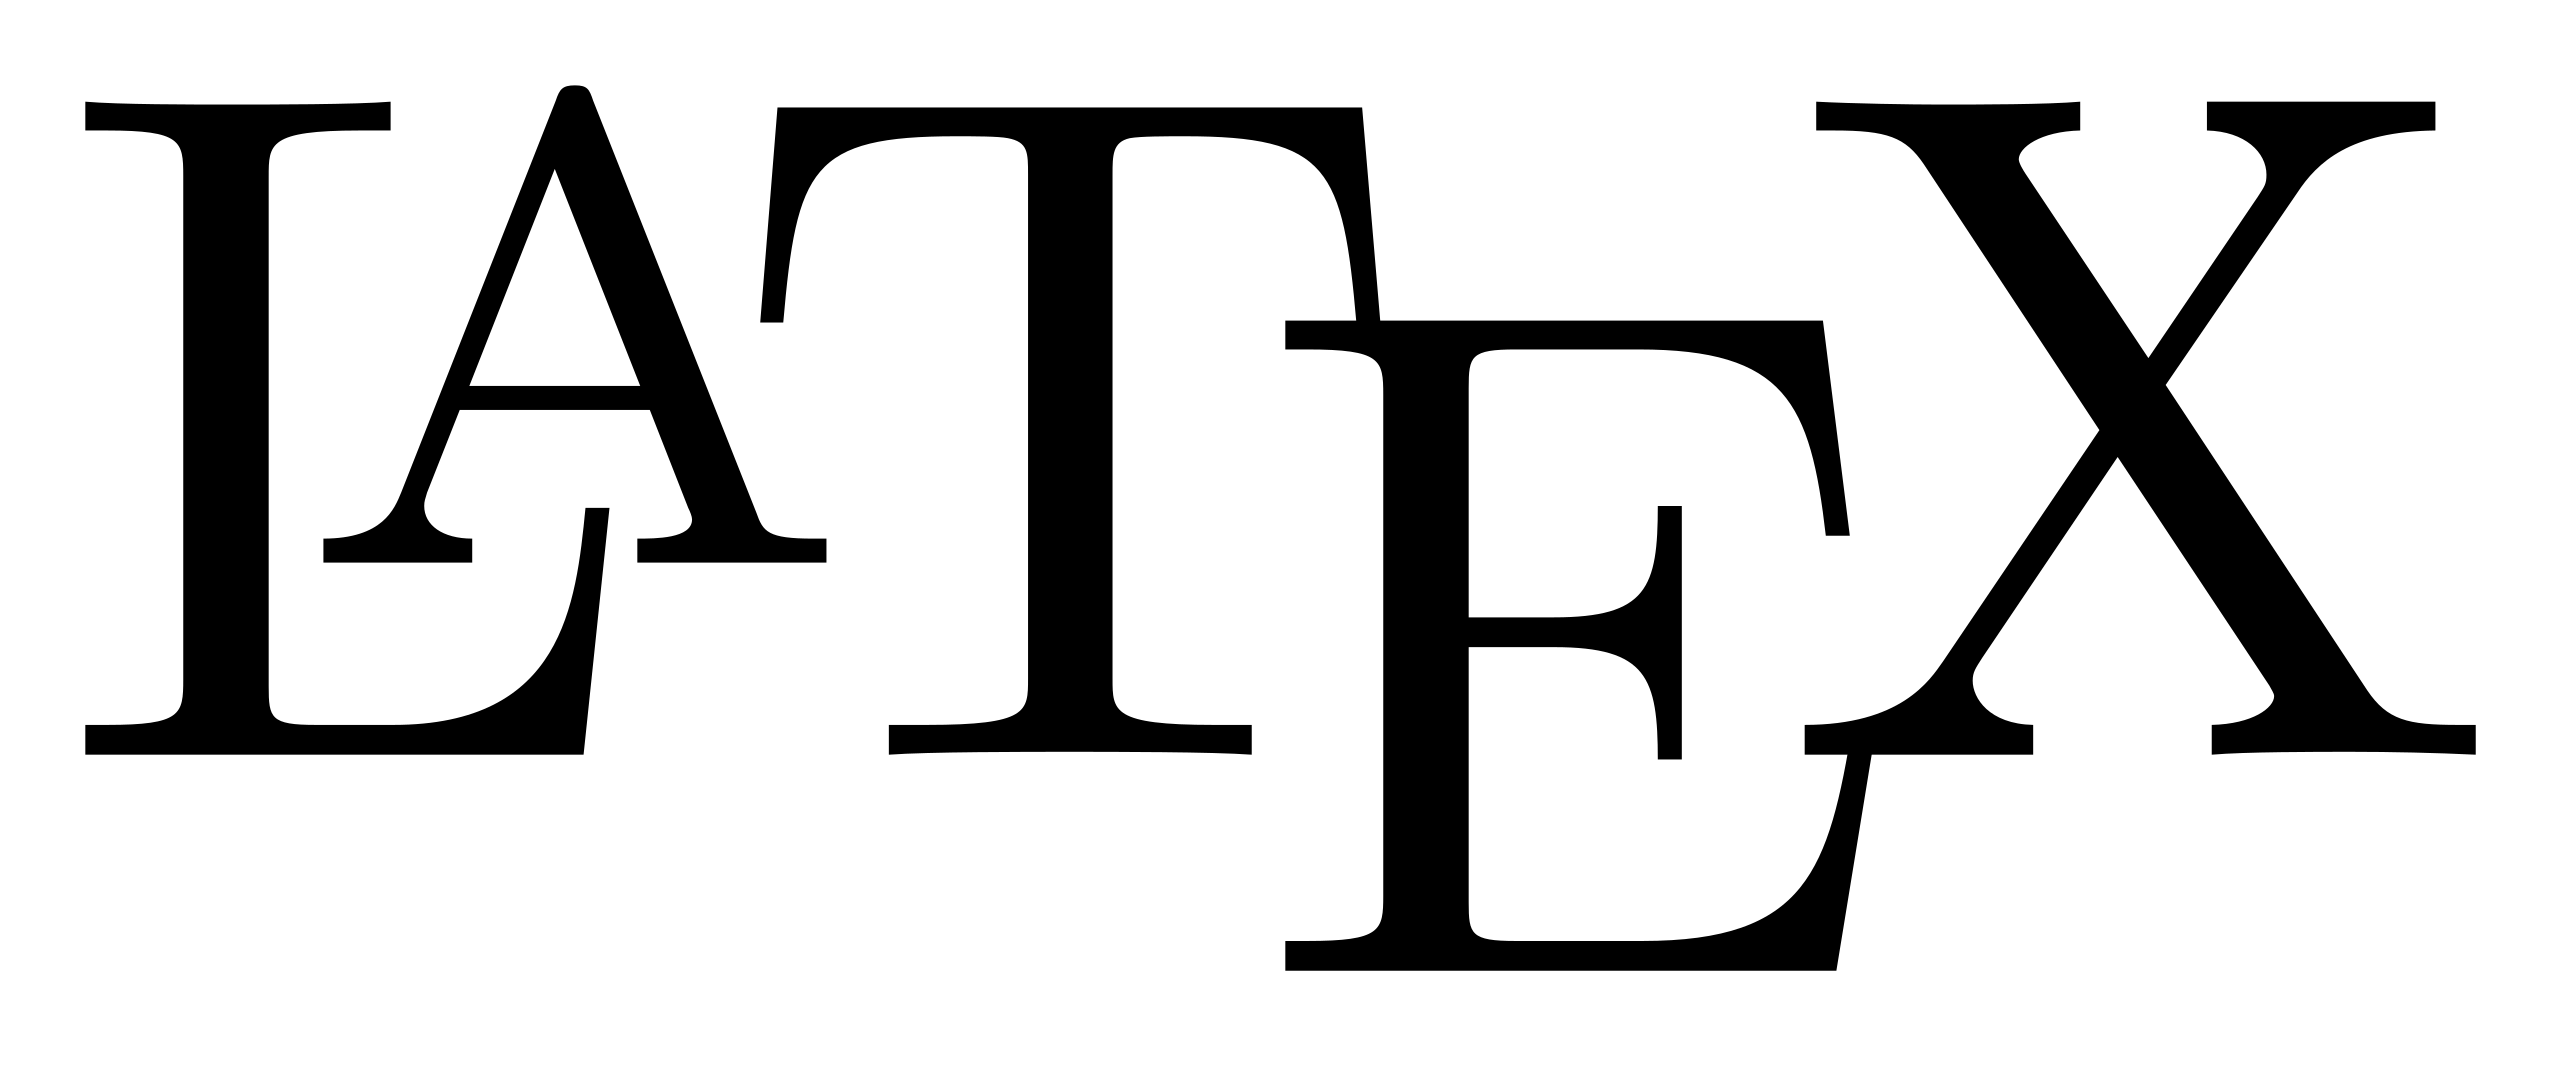
\includegraphics[width = 2cm , height=2cm]{img/techno/latex.png}}
                    \caption{\\ Latex logo \cite{latex}}\label{Fig:Data1}
                \end{minipage}
                \begin{minipage}{0.60\textwidth}
                    \par LaTeX est à la fois un langage de balisage et un logiciel de composition de documents,
                     largement utilisé par la communauté scientifique.\\
                      il facilite la rédaction de documents volumineux comme les mémoires et les thèses\cite{latex}.
                \end{minipage}
            \end{figure}
            \item\textbf{Draw.io:}
            %code image 
             \begin{figure}[!htb]\centering
                \begin{minipage}{0.30\textwidth}
                \centering
                    {
\includegraphics[width = 2cm , height=2cm]{img/techno/draw.png}}
                    \caption{\\ Draw.io logo \cite{draw}}\label{Fig:Data1}
                \end{minipage}
                \begin{minipage}{0.60\textwidth}
                    \par Draw.io est une application en ligne gratuite, accessible via un navigateur web (protocole https), permettant de dessiner des diagrammes et des organigrammes. \\
                    Cet outil offre la possibilité de concevoir toutes sortes de diagrammes et de dessins vectoriels, de les enregistrer au format XML, puis de les exporter \cite{draw}.
                    \end{minipage}
            \end{figure}
            \end{itemize}
\section{Réalisation}
\par Dans cette section, nous allons présenter la réalisation de ce projet en illustant chaque partie avec des captures explicatifs.
\subsection{Micro-service << Authentification\_Service >>}
\par Le micro-service << Authentification\_Service >> est responsable du système d'authentification de notre application 
\begin{itemize}
    \item \textbf{La liste des APIs:}
        \par La liste des APIs présents dans le micro-service d'authentification, documentée par Swagger, sont representés par la figure \textbf{\ref{fig:apiAuth}} suivante:
        \begin{figure}[H]
            \centering
            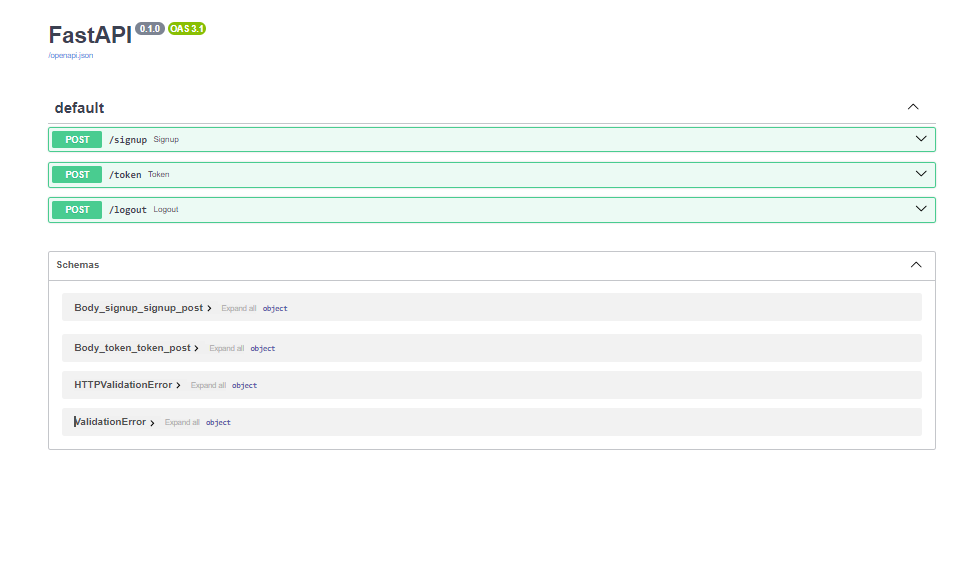
\includegraphics[width =1\linewidth, height=11cm]{img/captures/auth_apis.PNG}
            \caption{Liste des APIs du microservice <<Athentification\_service>> }
                \label{fig:apiAuth}
        \end{figure}
        \item \textbf{Interface de Création de compte <<Sign up>>:}
        \par L'interface de << Sign up>> est representée par la figure \textbf{\ref{fig:signup}} suivante:
        \begin{figure}[H]
            \centering
            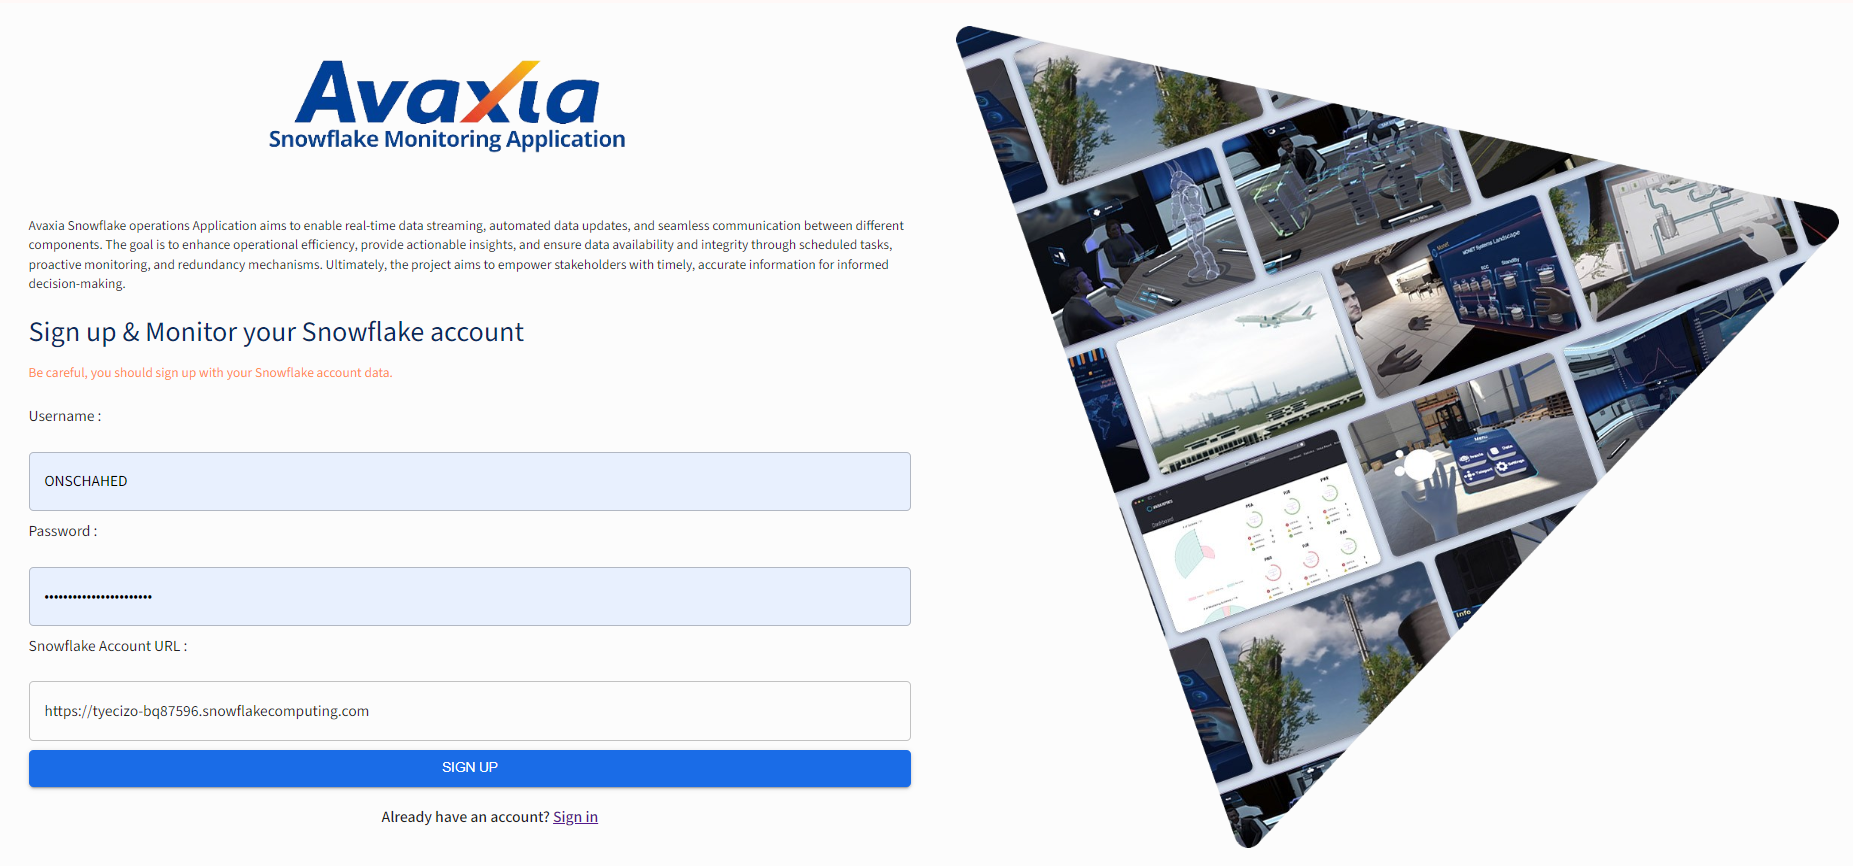
\includegraphics[width =1\linewidth]{img/captures/auth/signup.png}
            \caption{Interface de Création de compte <<Sign up>> }
                \label{fig:signup}
            \end{figure}
            \par Afin de créer un compte, l'utilisateur accède à cette interface en remplissant un formulaire d'inscription avec les données spécifiques à son compte Snowflake (username,mot de passe,l'url de connexion de son compte snowflake).
            Une fois l'utilisateur clique sur le bouton <<SINGUP>>, si les données sont valides: le système redirige l'utilisateur vers la page d'authentification. Sinon, il relance cette interface.
            \item \textbf{Interface d'authentification  <<Login>>:}
            \par L'interface de <<Login>> est representée par la figure \textbf{\ref{fig:login}} suivante:
            \begin{figure}[H]
                \centering
                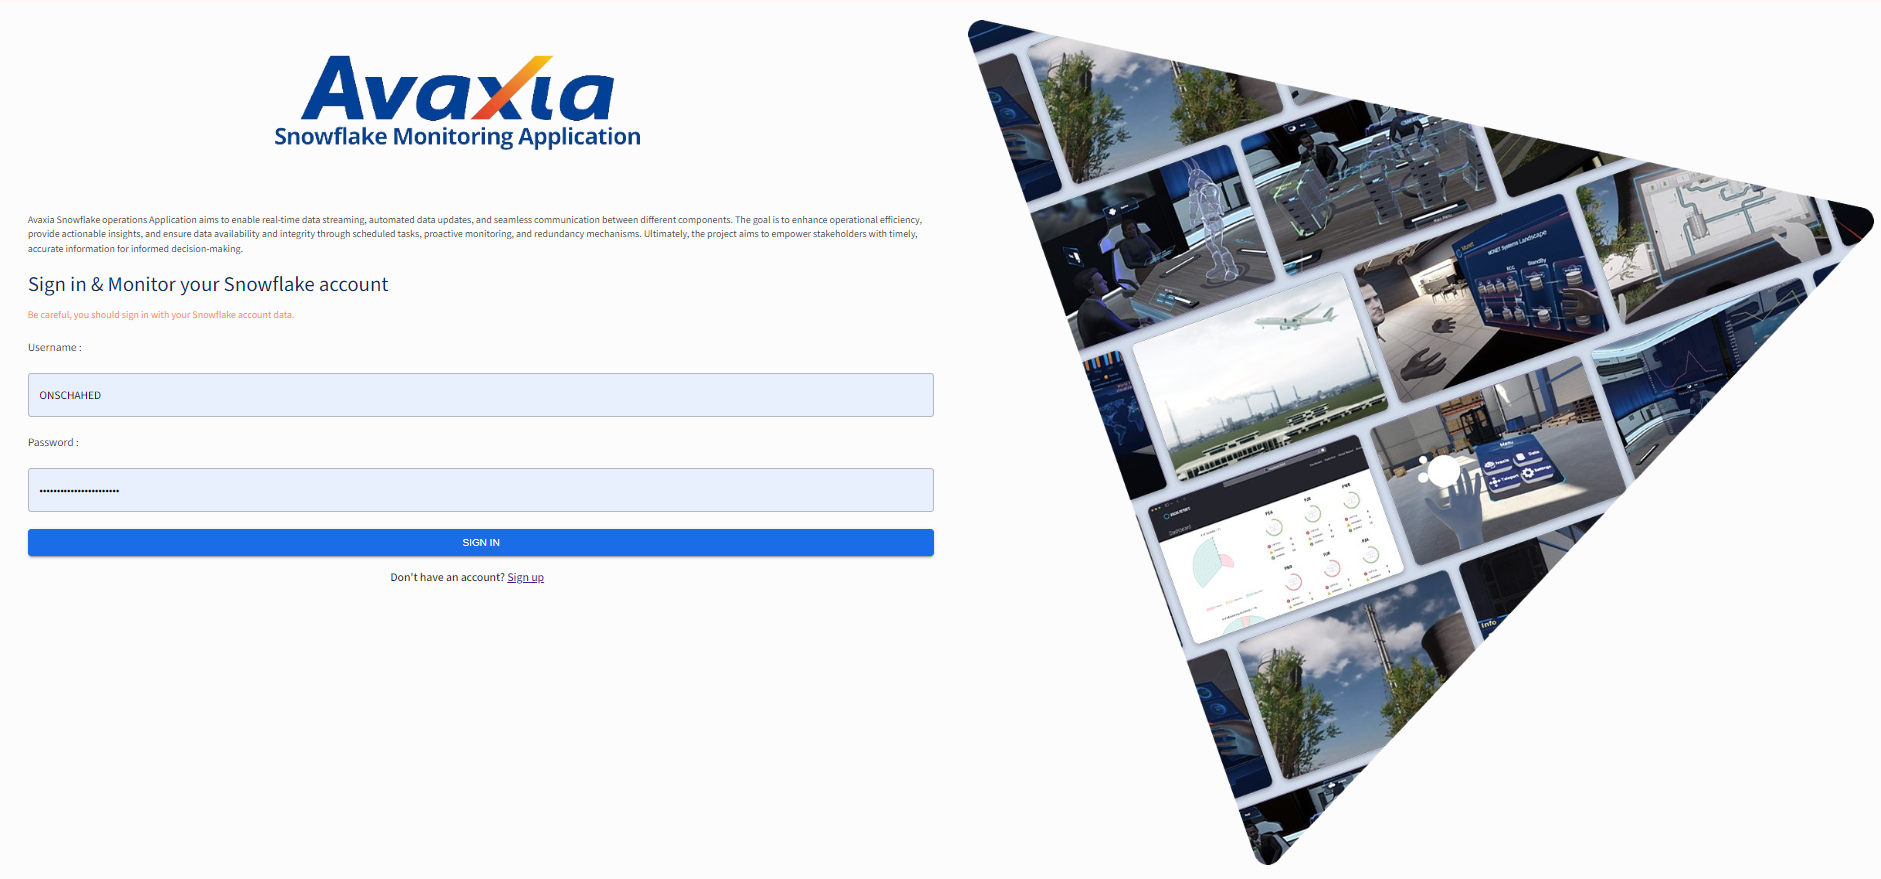
\includegraphics[width =1\linewidth]{img/captures/auth/login.png}
                \caption{Interface d'authentification  <<Login>>}
                    \label{fig:login}
                \end{figure}
                \par Pour accéder a son compte, l'utilisateur remplit le formulaire avec son <<username>> et <<mot de passe>>. Une fois les données sont valides, le système attribut une token d'accées à cet utilisateur et le redirige vers la page d'acceuil. Sinon, il relance la page de <<login>> en indiquant l'erreur.
                \par Si l'utilisateur est authentifié et clique sur le bouton <<Logout>>, indiqué dans la figure \textbf{\ref{fig:logout}}, il est redirigé vers l'interface de login automatiquement.
                \begin{figure}[H]
                    \centering
                    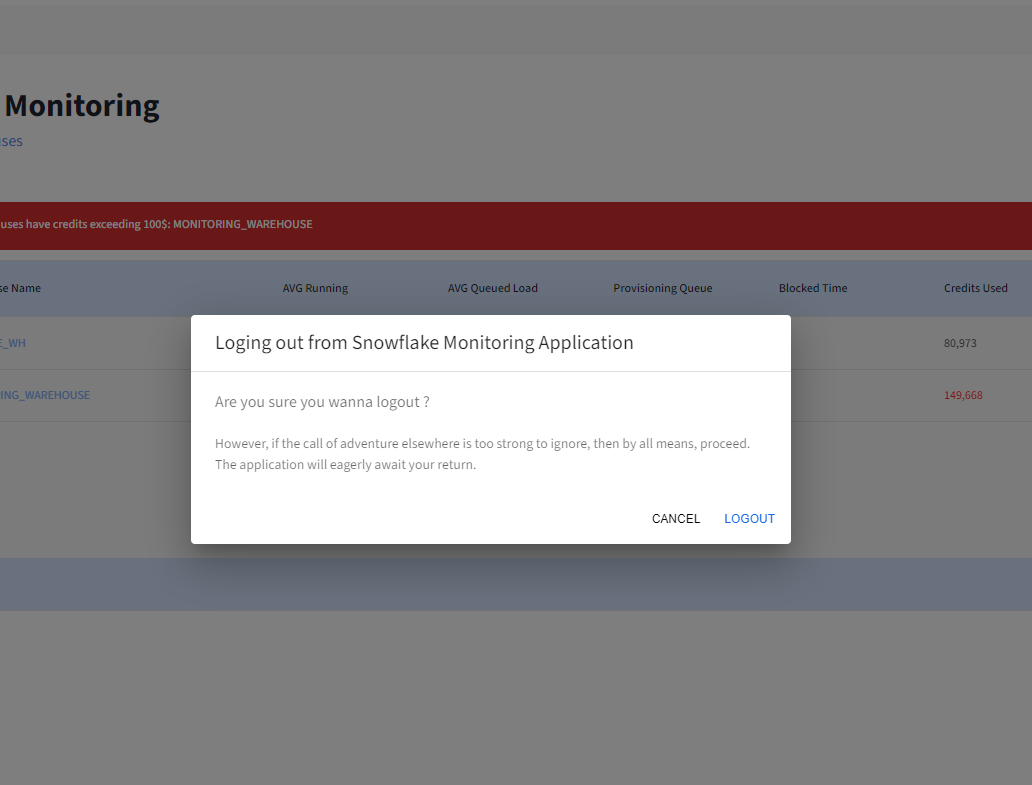
\includegraphics[width =0.8\linewidth]{img/captures/auth/logout.png}
                    \caption{ <<Logout>>}
                        \label{fig:logout}
                    \end{figure}
            \end{itemize}
\subsection{Micro-service << Warehouse\_Monitoring >>}
\par Le micro-service << Monitoring\_Service >> est le service chargé de la surveillance de l'utilisation des entrepôts de données Snowflake.
\begin{itemize}
    \item \textbf{La liste des APIs:}
        \par La liste des APIs présents dans ce micro-service, documentée par Swagger, sont representés par la figure \textbf{\ref{fig:apiWare}} suivante:
        \begin{figure}[H]
            \centering
            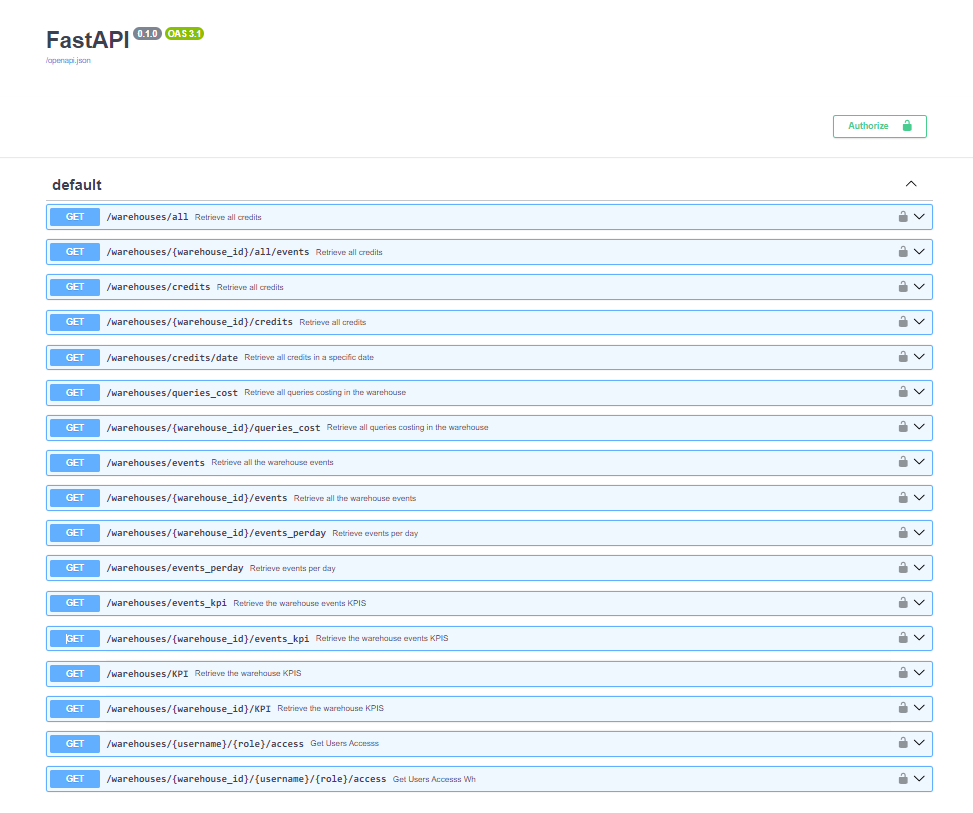
\includegraphics[width =1\linewidth]{img/captures/warehouses_apis.PNG}
            \caption{Liste des APIs du microservice <<Warehouse\_Monitoring>> }
                \label{fig:apiWare}
        \end{figure}

        \item \textbf{Interface de la liste des entrepôts de données:}
        \par L'interface de  de la liste des entrepôts de données est representée par la figure \textbf{\ref{fig:warehouse1}} suivante:
        \begin{figure}[H]
            \centering
            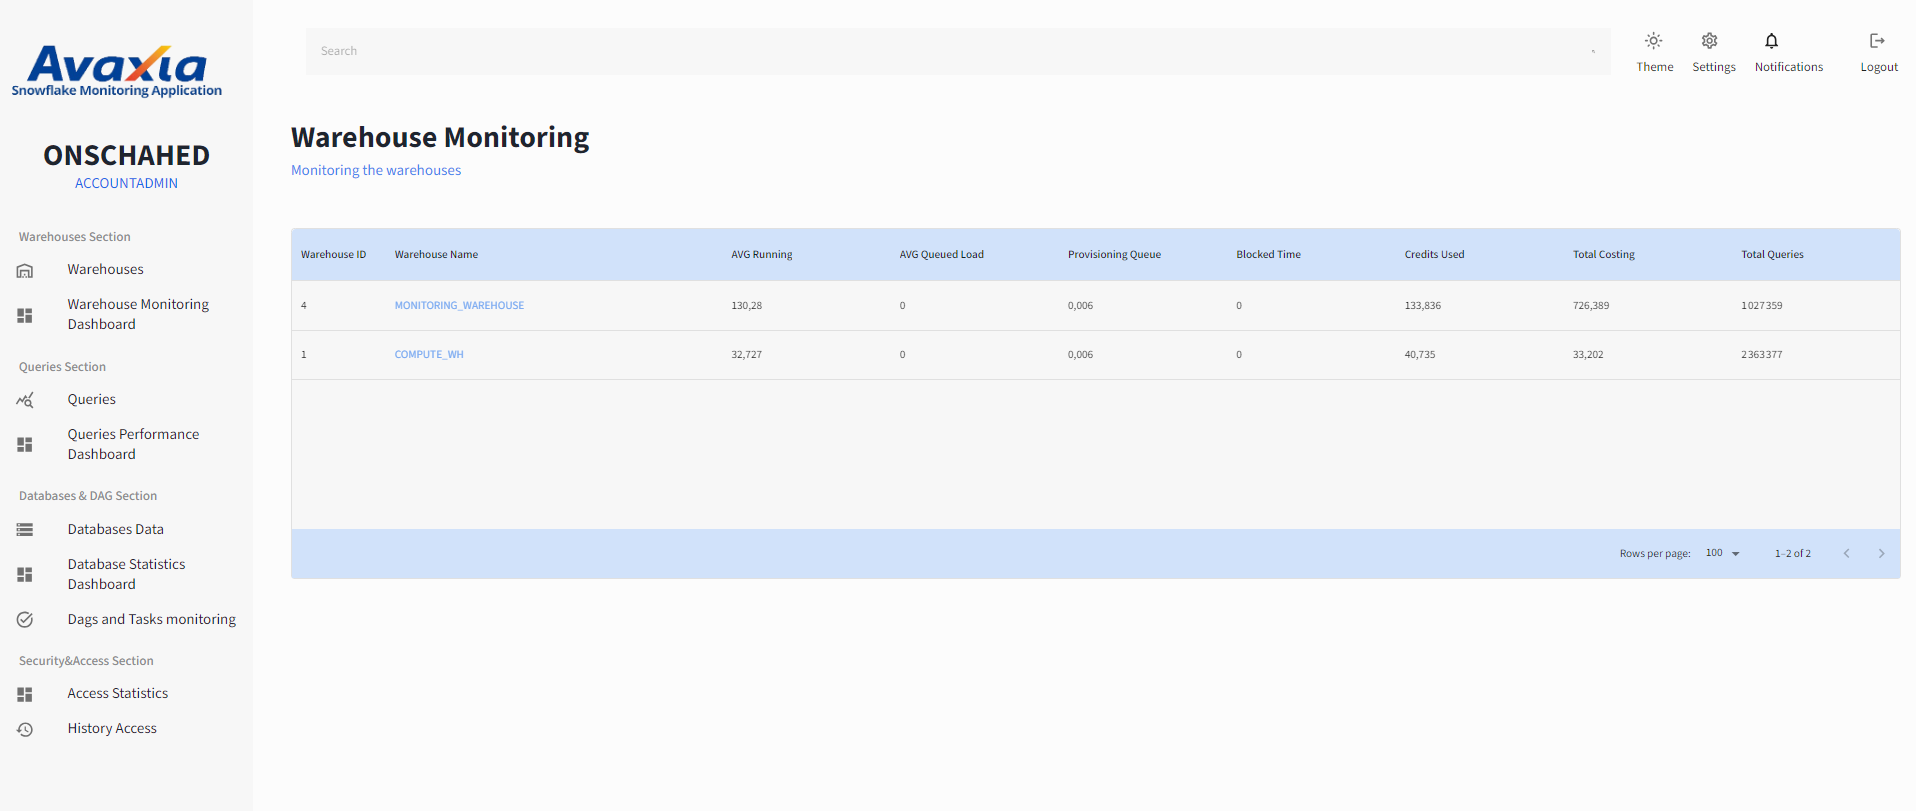
\includegraphics[width =1\linewidth]{img/captures/warehouse/liste.png}
            \caption{Interface de la liste des entrepôts de données}
                \label{fig:warehouse1}
            \end{figure}
            \par Le tableau présente des informations détaillées sur les différents entrepôts surveillés, notamment leur ID, leur nom, leurs métriques de performance (débit moyen, charge moyenne, file d'attente de provisionnement, temps bloqué, crédits utilisés, coût total) ainsi que le nombre total de requêtes. \\
            \item \textbf{Tableau de bord du surveillance des entrepôts des données}
            \par Les deux tableaux de bord du surveillance des entrepôts des données \textbf{<<Monitoring\_warehouse>>} et \textbf{<<Compute\_WH>>} sont representées par les deux figures \textbf{\ref{fig:warehouse2}} et \textbf{\ref{fig:warehouse3}}:
                \begin{figure}[H]
                    \centering
                    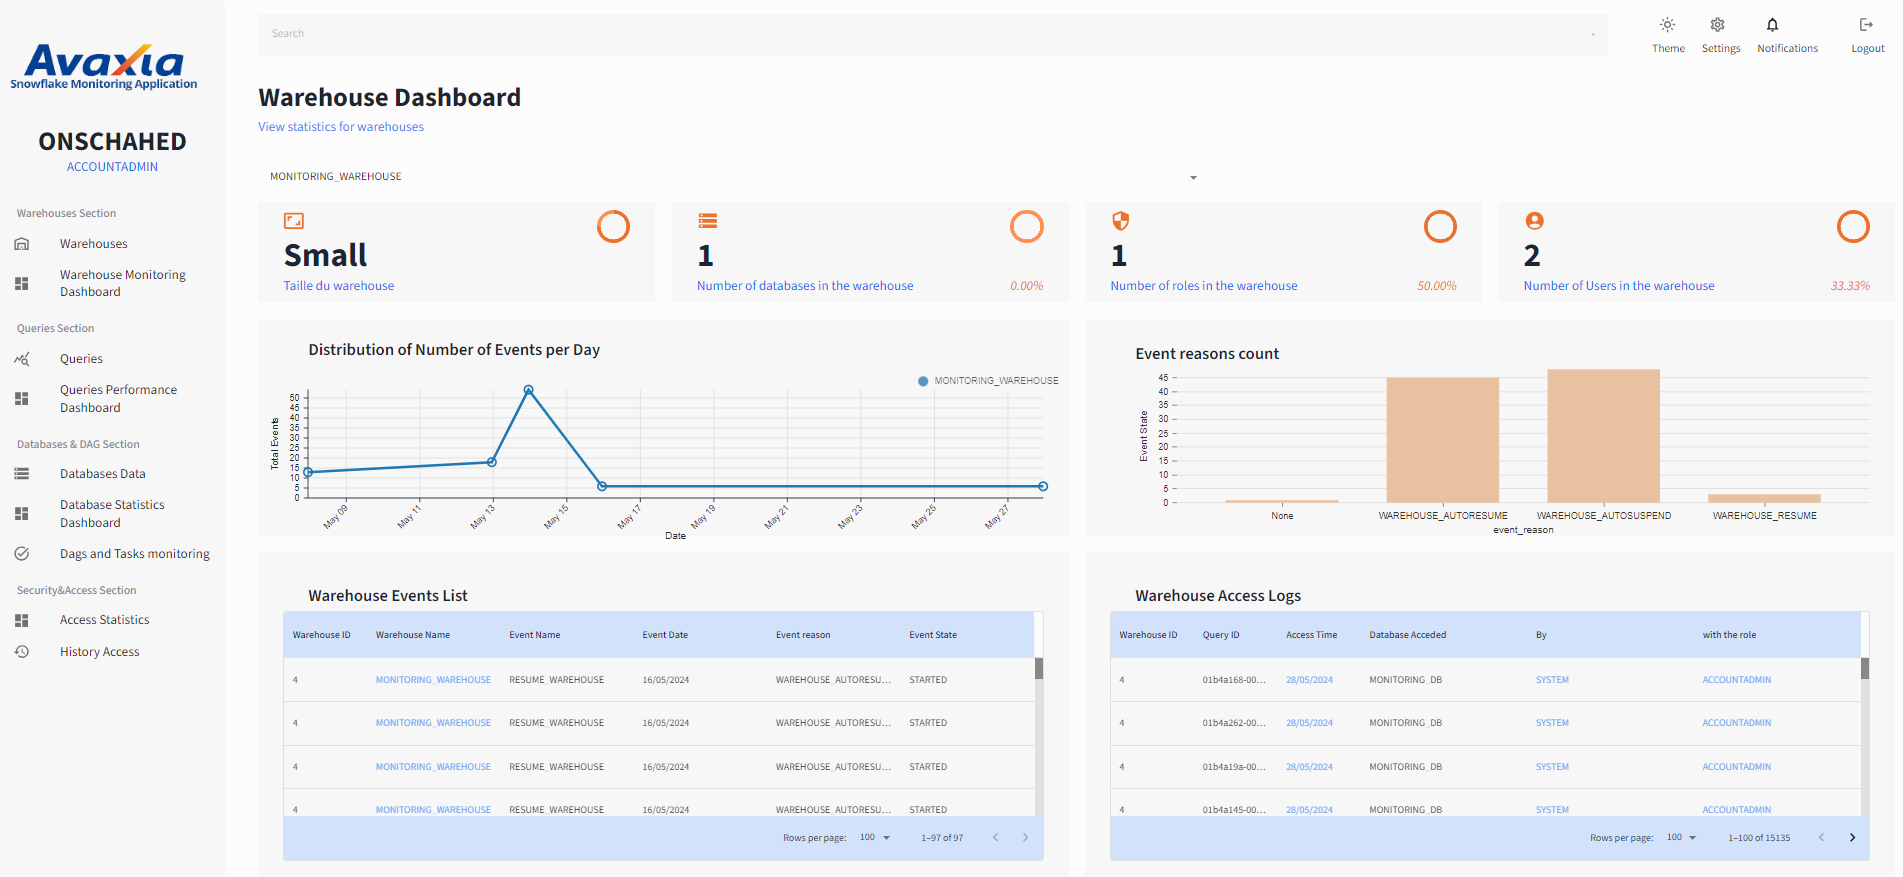
\includegraphics[width =1\linewidth]{img/captures/warehouse/warehouse_dash.png}
                    \caption{Tableau de bord du surveillance d l'entrepôts des données <<Monitoring\_warehouse>>}
                        \label{fig:warehouse2}
                \end{figure}
                \begin{figure}[H]
                    \centering
                    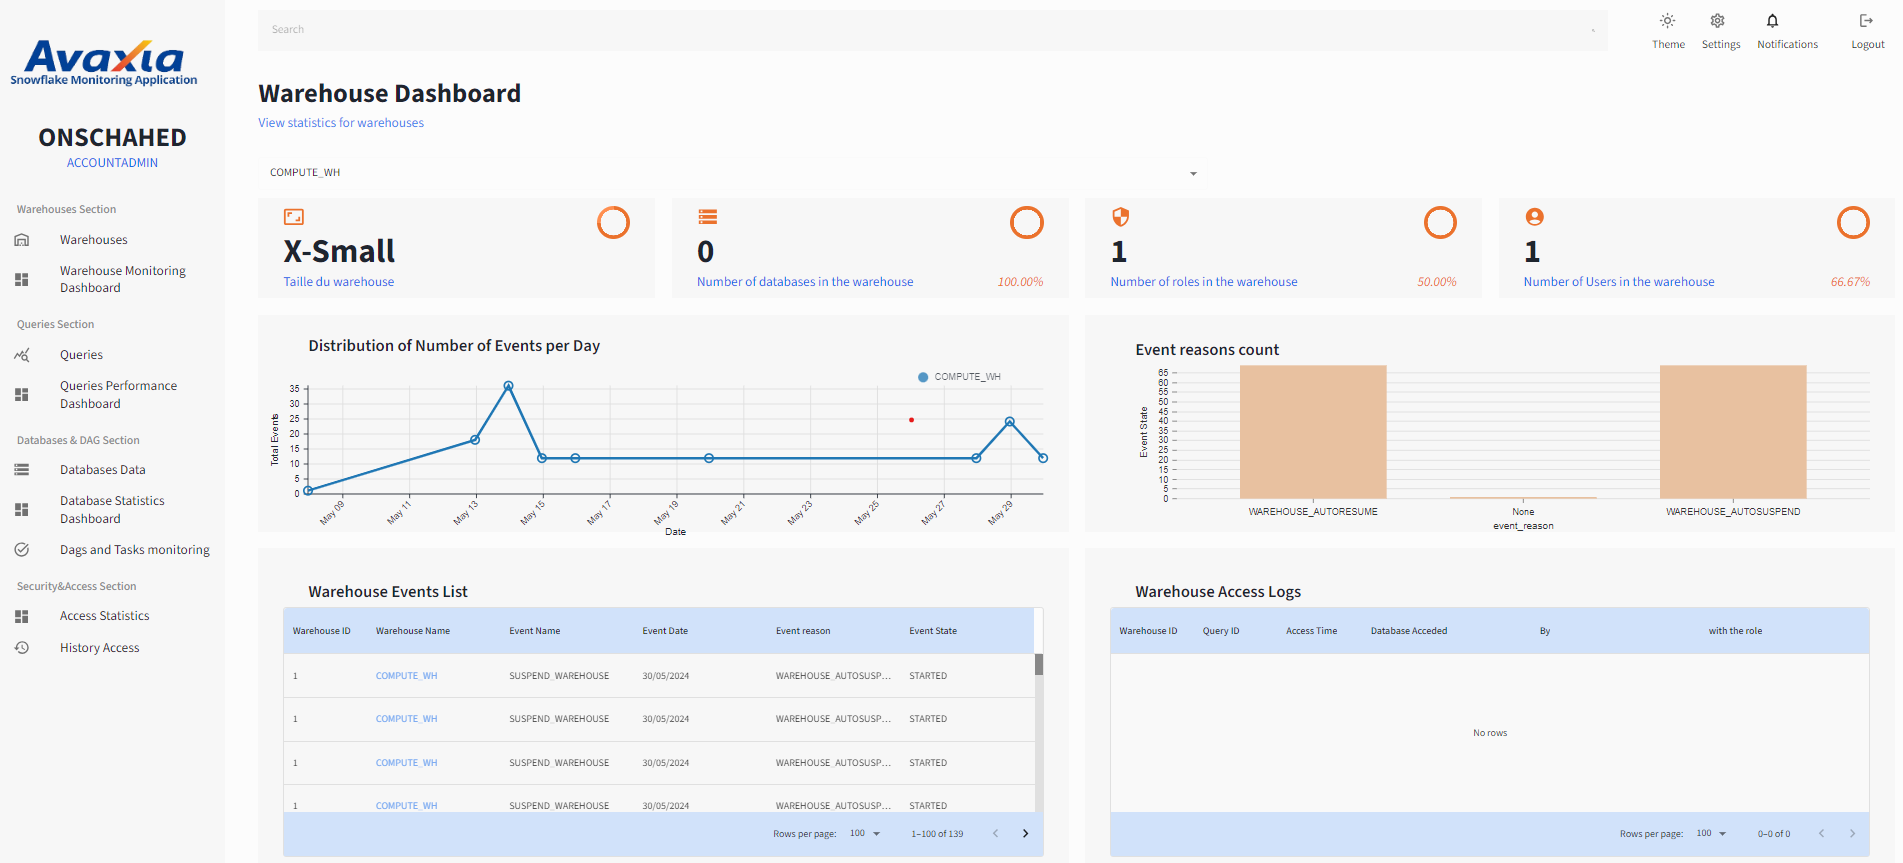
\includegraphics[width =1\linewidth]{img/captures/warehouse/compute.png}
                    \caption{Tableau de bord du surveillance d l'entrepôts des données <<Compute\_WH>>}
                        \label{fig:warehouse3}
                \end{figure}
                \par Ces tableaux de bord des entrepôts Snowflake offrent un aperçu complet des activités et de l'utilisation de l'infrastructure de données. Ils présentent des informations clés sur la taille, la composition et l'utilisation des entrepôts, notamment le nombre de bases de données, nombre des evenments effectuées dans l'entrepôt ainsi que le nombre de rôles et d'utilisateurs.
                
                 
            \item \textbf{Changement des variables globaux}
            \par Le changement des paramétres globaux peut reflecter les vues de ce micro service une fenêtre s'affiche lorsque on clique sur le bouton <<Settings>> du topbar. Selon les besoins de l'utilisateur/administrateur  :
                \begin{enumerate}
                    \item[-] \textbf{Changement du rôle d'utilisateur/Administrateur:}
                    \begin{figure}[H]
                        \centering
                        \begin{tabular}[b]{c}
                        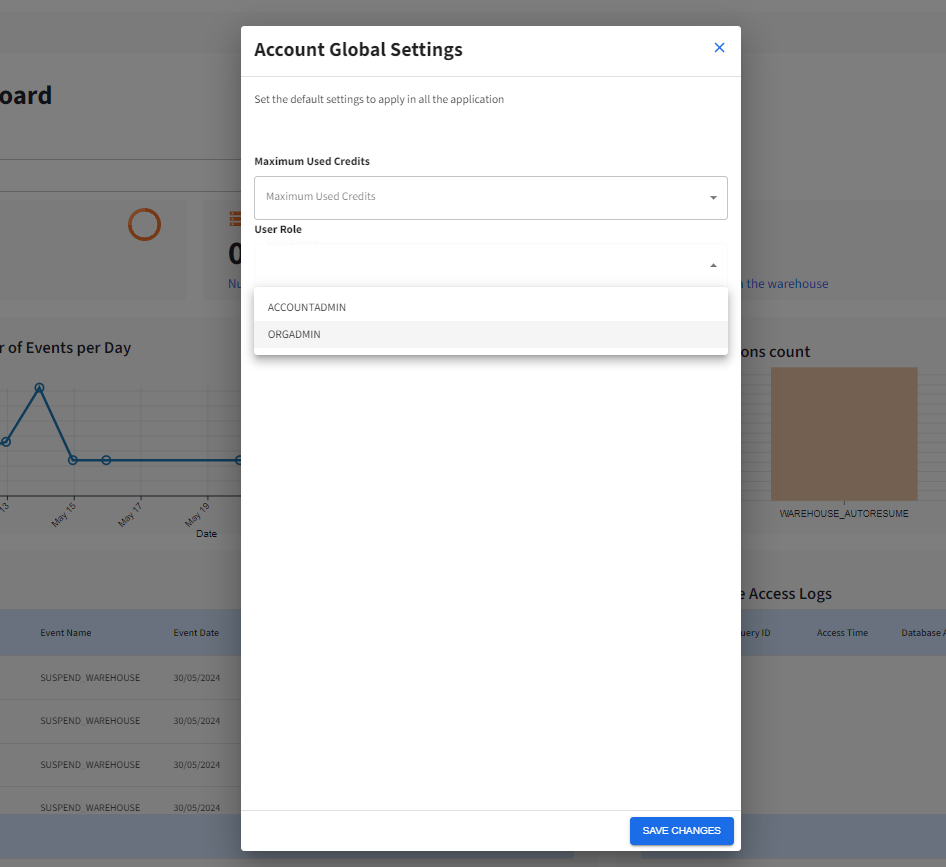
\includegraphics[width=.3\linewidth, height=5cm]{img/captures/warehouse/global_set_role.png} \\
                        
                        \end{tabular} 
                        \begin{tabular}[b]{c}
                        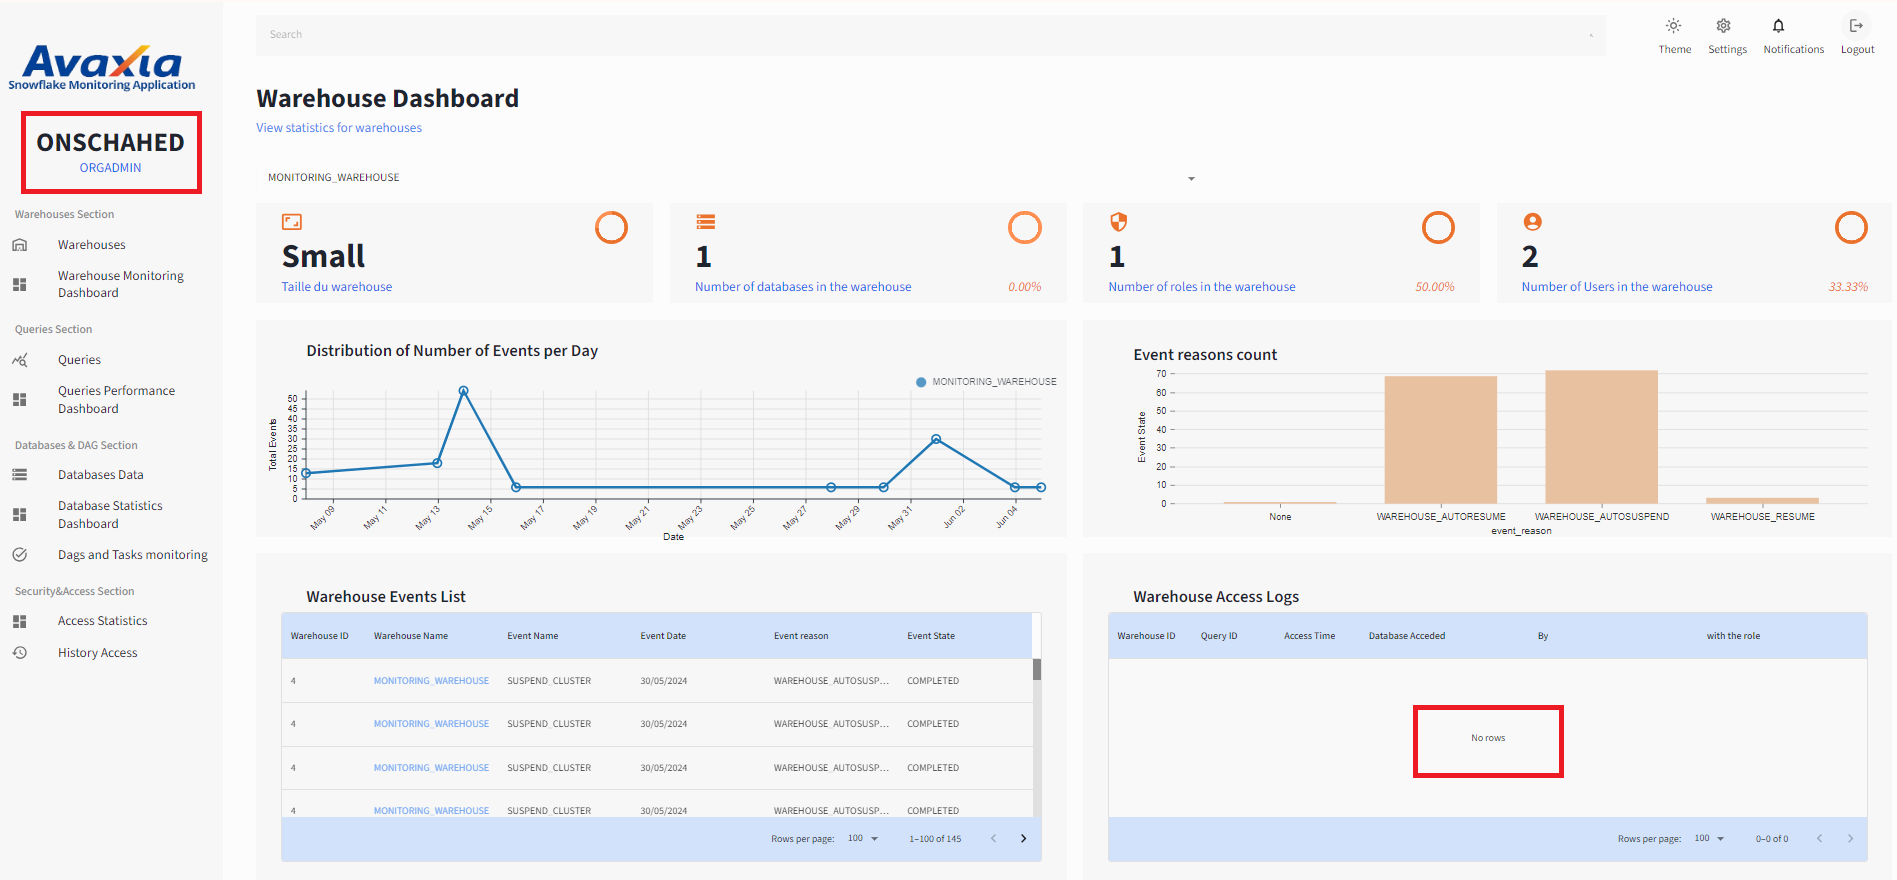
\includegraphics[width=.6\linewidth, height=5cm]{img/captures/warehouse/sysorg.png} \\
                        
                        \end{tabular}
                        \caption{Changement du role de l'utilisateur de <<ACCOUNT ADMIN>> vers <<ORGADMIN>>                    }
                    \end{figure}
                    \par Lorsque l'utilisateur  modifit les paramètres globaux, telque le rôle de compte utilisateur, les journaux d'accès aux entrepôts ne sont plus affichés dans cette interface. Cela signifie que les administrateurs doivent être conscients que certaines informations peuvent ne pas être visibles dans certaines configurations.
                    \item[-] \textbf{Changement du seuil maximum des crédits d'utilisation:}
                    \begin{figure}[H]
                        \centering
                        \begin{tabular}[b]{c}
                        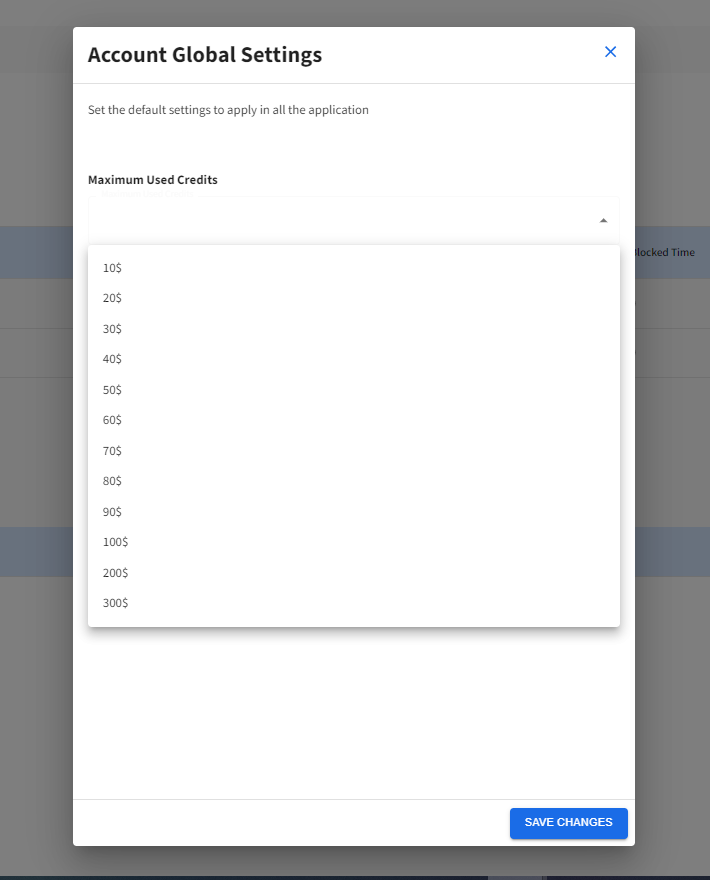
\includegraphics[width=.2\linewidth, height=5.5cm]{img/captures/warehouse/global_set_credits.png} \\
                        
                        \end{tabular} 
                        \begin{tabular}[b]{c}
                        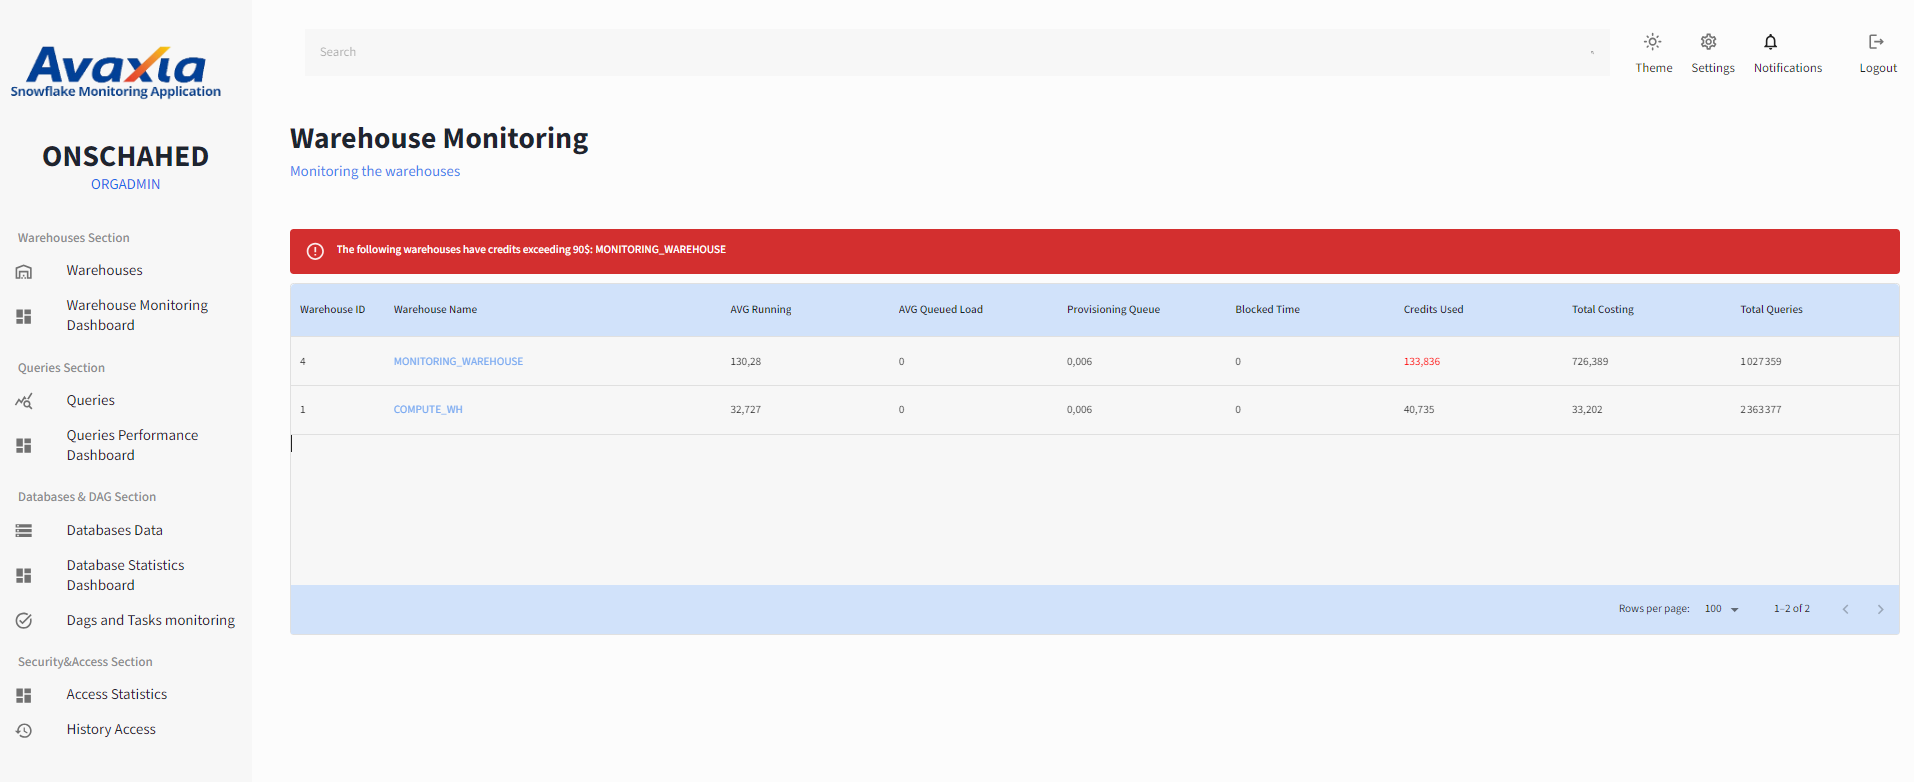
\includegraphics[width=.7\linewidth, height=5.5cm]{img/captures/warehouse/90.png} \\
                        
                        \end{tabular}
                        \caption{Changement de seuil de credits vers <<90\$>>                    }
                    \end{figure}
                    \par Lorsque l'utilisateur modifie les paramètres globaux, notamment le seuil de crédits maximum utilisés, une notification permanente devrait être affichée si les crédits utilisées de l'un des entrepôt de donneés à depacer cette seuil pour informer l'utilisateur de cette malveuillance.
            \end{enumerate}

\end{itemize}
\par Dans l'ensemble, cet microservice offre une visibilité essentielle sur les performances et l'utilisation des entrepôts, facilitant la prise de décisions éclairées pour l'infrastructure de données.
\subsection{Micro-service << Query\_Performance >>}
\par Le micro-service << Monitoring\_Service >> est le service chargé de la surveillance des requêtes SQL effectuées au sein du compte Snowflake.
\begin{itemize}
    \item \textbf{La liste des APIs:}
        \par La liste des APIs présents dans ce micro-service, documentée par Swagger, sont representés par la figure \textbf{\ref{fig:apiquery}} suivante:
        \begin{figure}[H]
            \centering
            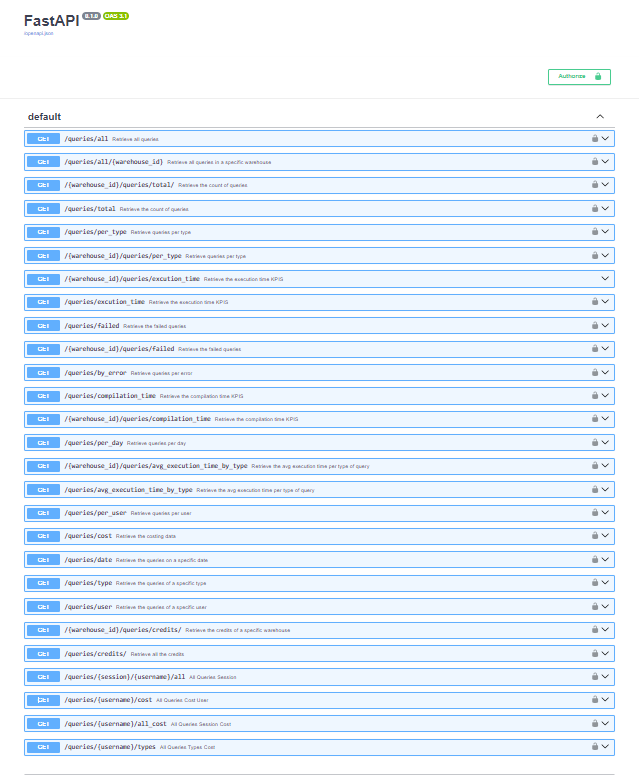
\includegraphics[width =1\linewidth]{img/captures/queries_apis.PNG}
            \caption{Liste des APIs du microservice <<Warehouse\_Monitoring>> }
                \label{fig:apiquery}
        \end{figure}

        \item \textbf{Interface de historique des requêtes de l'utilisateur:}
        \par L'interface de la liste des entrepôts de données est representée par la figure \textbf{\ref{fig:listqueries}} suivante:
        \begin{figure}[H]
            \centering
            \includegraphics[width =1\linewidth]{img/captures/queries/queries_list.png}
            \caption{Interface de la liste des entrepôts de données}
                \label{fig:listqueries}
            \end{figure}
            \par Cette vue représente l'historique des requêtes dans l'application de surveillance Snowflake.
             Elle fournit un aperçu détaillé de chaque requête exécutée. \\ 
             Cet l'historique permet aux administrateurs de surveiller en détail les requêtes exécutées afin de pouvoir identifier les éventuels problèmes liés aux ces derniers dans le compte Snowflake en question.
            \item \textbf{Tableaux de bord du surveillance des Requêtes SQL}
            \begin{enumerate}
                \item[-] \textbf{Les informations générale sur la totalité des requêtes dans le compte de l'utilisateur:  }
                    \par La figure \textbf{\ref{fig:queriesglob}} illustre le tableau de bord global des requêtes SQL du compte Snowflake:
                    \begin{figure}[H]
                        \centering
                        \includegraphics[width =1\linewidth]{img/captures/queries/global_queries_dash.png}
                        \caption{Tableau de bord du surveillance des entrepôts des données}
                            \label{fig:queriesglob}
                    \end{figure}
                    \item[-] \textbf{Selection  de l'entrepôts des données appriori:}
                    
                    \par Une fois l'utilisateur selectionne un entrepôt de données, depuis la liste de ces entrepôts, qui s'affiche en cliquant sur la liste déroulante <<select warehouse>> comme l'indique la figure \textbf{\ref{fig:select}}, les données spécifique à cet entrepôt vont être affichées.
                    \begin{figure}[H]
                        \centering
                        \includegraphics[width =1\linewidth]{img/captures/queries/queries_selection_warehouse.png}
                        \caption{Tableau de bord du surveillance des entrepôts des données}
                            \label{fig:select}
                    \end{figure}
                    \par La figure \textbf{\ref{fig:queriesdash1}} illustre le tableau de bord de l'entrepôt <<Monitoring\_Warehouse>>:
                    \begin{figure}[H]
                        \centering
                        \includegraphics[width =1\linewidth]{img/captures/queries/monitoring_dash.png}
                        \caption{Tableau de bord du surveillance de l'entrepôt des données <<Monitoring\_Warehouse>> }
                            \label{fig:queriesdash1}
                    \end{figure}
                    \par La figure \textbf{\ref{fig:queriesdash2}} illustre le tableau de bord de l'entrepôt <<Compute\_WH>>:
                    \begin{figure}[H]
                        \centering
                        \includegraphics[width =1\linewidth]{img/captures/queries/compute_dash.png}
                        \caption{Tableau de bord du surveillance de l'entrepôt des données <<Compute\_WH>>}
                            \label{fig:queriesdash2}
                    \end{figure}
                    \par ces tableaux de bord présentent des indicateurs clés sur les requêtes exécutées, tels que le nombre total de requêtes, le coût total, le temps d'exécution moyen et le taux de requêtes en échec. Cette vision synthétique permet aux administrateurs d'avoir une compréhension globale des performances.
                    \\ Les graphiques complémentaires apportent une analyse approfondie des tendances par type de requête. Ils montrent la variation du temps d'exécution et de compilation, ainsi que la répartition du nombre total de requêtes et du temps d'exécution par type de requête. Cette granularité permet d'identifier les domaines à optimiser pour améliorer l'efficacité du système.
            \end{enumerate}

\end{itemize}
\par Le service  << Query\_Performance >> constitue un outil essentiel pour les équipes en charge de l'exploitation et de l'optimisation de l'infrastructure Snowflake. Il offre une visibilité complète sur les activités de requêtes, permettant de prendre des décisions éclairées afin d'améliorer la fiabilité, les performances et la rentabilité globale du système.
\subsection{Micro-service << Databases\_Statistics >>}
\par Le micro-service << Databases\_Statistics >> est le service chargé de la surveillance des base de données créees au sein du compte Snowflake.
\begin{itemize}
    \item \textbf{La liste des APIs:}
        \par La liste des APIs présents dans ce micro-service, documentée par Swagger, sont representés par la figure \textbf{\ref{fig:apiData}} suivante:
        \begin{figure}[H]
            \centering
            \includegraphics[width =1\linewidth]{img/captures/database_apis.PNG}
            \caption{Liste des APIs du microservice<< Databases\_Statistics >> }
                \label{fig:apiData}
        \end{figure}

        \item \textbf{La liste des bases de données et ces diffrents schémas:}
        \par L'interface de la liste des bases de données et ces diffrents schémas est representée par la figure \textbf{\ref{fig:dblist}} suivante:
        \begin{figure}[H]
            \centering
            \includegraphics[width =1\linewidth]{img/captures/database/1.png}
            \caption{La liste des bases de données}
                \label{fig:dblist}
            \end{figure}
            \par La section "List of Databases" affiche les détails des différentes bases de données, y compris leur ID, leur nom, leur propriétaire et leurs dates de création et de dernière modification.\\ 
            Une fois l'utilisateur selectionne une base de données, La liste des schémas d'affiche comme l'indique la figure \textbf{\ref{fig:schemas}} suivante:
                \begin{figure}[H]
                \centering
                \includegraphics[width =1\linewidth]{img/captures/database/2.png}
                \caption{Liste des schémas de base de données}
                    \label{fig:schemas}
                \end{figure}

             Ensuite, pour qu'on puisse lister les objets présents et créeés dans cette base de données, l'utilisateur selectionne le schéma appriori pour lister ces objets.
            \par La figure \textbf{\ref{fig:objects}} ilusstre cette action:
            \begin{figure}[H]
                \centering
                \includegraphics[width =1\linewidth]{img/captures/database/3.png}
                \caption{Liste des objets dans la base de données}
                    \label{fig:objects}
                \end{figure}
            \par Ces informations permettent aux administrateurs de l'application de surveiller et de gérer son compte Snowflake, en ayant une vue d'ensemble des bases de données, des schémas et des objets utilisés dans le système de surveillance.
             \item \textbf{Tableaux de bord du surveillance des bases de données:}
             \par La figure \textbf{\ref{fig:dashdata}} représente le tableau de bord du surveillance des bases de données:
             \begin{figure}[H]
                \centering
                \includegraphics[width =1\linewidth]{img/captures/database/database_dash.png}
                \caption{Tableaux de bord du surveillance des bases de données}
                    \label{fig:objects}
                \end{figure}
                \par Cette interface de tableau de bord des statistiques des bases de données fournit une vue d'ensemble complète des principales métriques liées à l'utilisation et à la gestion des données dans l'environnement Snowflake. 
                Elle présente des indicateurs clés tels que le nombre de tables, le coût total des bases de données, le stockage total utilisé et le nombre total de requêtes affectées.
                Les graphiques détaillés complètent ces informations en montrant l'évolution de l'utilisation du stockage, la répartition des types d'objets de base de données, la distribution des bases de données par rôle et par type, ainsi que l'évolution du coût quotidien des requêtes. \\ 
                
\end{itemize}
\par Ce microservice  offre aux administrateurs un outil complet et puissant pour surveiller les performances des bases de données, identifier les tendances clés et prendre des décisions éclairées afin d'optimiser l'utilisation et la gestion des coûts de leurs comptes.
\subsection{Micro-service << Access\_Statistics >>}
\par Le micro-service << Access\_Statistics >>  est le service chargé de la surveillance des access aux comptes Snowflake.
\begin{itemize}
    \item \textbf{La liste des APIs:}
        \par La liste des APIs présents dans ce micro-service, documentée par Swagger, sont representés par la figure \textbf{\ref{fig:apiAccess}} suivante:
        \begin{figure}[H]
            \centering
            \includegraphics[width =1\linewidth]{img/captures/access_apis.PNG}
            \caption{Liste des APIs du microservice << Access\_Statistics >> }
                \label{fig:apiAccess}
        \end{figure}

        \item \textbf{L'historique des accées de l'utilisateur ONS CHAHED:}
        \par L'interface de l'historique d'accées est representée par la figure \textbf{\ref{fig:accesslist}} suivante:
        \begin{figure}[H]
            \centering
            \includegraphics[width =1\linewidth]{img/captures/user/history.png}
            \caption{Historique des accées}
                \label{fig:accesslist}
            \end{figure}
            \par Cette interface d'historique des accès fournit une traçabilité complète des activités dans l'environnement Snowflake. 
            Elle enregistre de manière détaillée chaque événement d'accès, capturant des informations clés telles que l'identité de l'utilisateur, l'heure d'accès et les méthodes d'authentification utilisées. \\
            Ce journal d'activité exhaustif représente un outil de gouvernance et de surveillance essentiel pour les administrateurs. 
            Il leur permet de suivre les mouvements des différents acteurs au sein du système, de détecter d'éventuelles activités suspectes et d'assurer la sécurité globale de l'infrastructure.
            \item \textbf{Tableaux de bord du surveillance des accéess des utilisateurs:}
             \par Les figures \textbf{\ref{fig:acess1}} et \textbf{\ref{fig:acess2}} représentent les tableaux de bord du surveillance des accées de l'utilisateur <<ONS CHAHED>> et l'utilisateur système <<Snowflake>>:
             \begin{figure}[H]
                \centering
                \includegraphics[width =1\linewidth]{img/captures/user/1.png}
                \caption{Tableau de bord du surveillance des accéess de l'utilisateur <<ONS CHAHED>>}
                    \label{fig:acess1}
                \end{figure}
                \begin{figure}[H]
                    \centering
                    \includegraphics[width =1\linewidth]{img/captures/user/2.png}
                    \caption{Tableau de bord du surveillance des accéess de l'utilisateur <<SNOWFLAKE>>}
                        \label{fig:acess1}
                    \end{figure}
                \par Ces tableaux de bord offrent une visibilité complète sur l'activité des différents utilisateurs au sein de l'environnement Snowflake. Ils permettent de suivre des indicateurs clés tels que le nombre de sessions, de requêtes exécutées, d'applications utilisées et les coûts associés. Ces données quantitatives fournissent une image détaillée de l'utilisation du système par chaque utilisateur.
                \\ L'historique détaillé des sessions et des requêtes autorisées complète ce tableau, donnant aux administrateurs une traçabilité exhaustive des actions entreprises par chaque utilisateur. Cet outil de suivi leur permet de détecter les éventuelles anomalies et de s'assurer du respect des politiques d'accès.
                Ils fournissent aux équipes opérationnelles les informations nécessaires pour prendre des décisions éclairées en matière de sécurité, de contrôle d'accès et d'utilisation des ressources.
\end{itemize}
\par Ce microservice de surveillance des accès est bien plus qu'un simple registre. C'est un levier puissant pour les équipes en charge de la gouvernance et de l'exploitation des systèmes de données, leur permettant de prendre des décisions éclairées et de maintenir la fiabilité et la résilience de l'environnement Snowflake dans le temps.
\subsection{Micro-service << DAG\_Monitoring >>}
\par C'est le service responsable du suivi et de la surveillance en temps réelle des flux de taches (<<DAG>>) exécutés et programmées dans Snowflake. 
\par Dans cette section, nous allons surveiller l'éxécution d'un ensemble des tâches en temps réelle. 
\\ Ces tâches la sont deja crées dans notre compte Snowflake de test,La figure \textbf{\ref{fig:show}} illustre la liste des tâches, dont nous allons monitorer, dans snowflake qui apparâitre en exécutant la command << Show TASKS >>:
    \begin{figure}[H]
            \centering
            \includegraphics[width =1\linewidth]{img/captures/dag/show.PNG}
            \caption{Résultat du command <<Show tasks>> }
                \label{fig:show}
        \end{figure}
    \par Simultanément, dans notre application, les tâches sont illustrés par la figure \textbf{\ref{fig:sus}} dans le même état <<SUSPENDED>> que dans snowflake:
    \begin{figure}[H]
        \centering
        \includegraphics[width =1\linewidth]{img/captures/dag/1/ok/0.png}
        \caption{Etat initial du DAG}
            \label{fig:sus}
    \end{figure}

\section*{Conclusion}
\addcontentsline{toc}{section}{Conclusion }
    Ce chapitre résume le travail accompli pour donner forme à notre projet. Les choix techniques et le workflow nous ont fourni un cadre solide pour concrétiser notre vision. Chaque étape de ce processus s'avère cruciale pour l'atteinte de nos objectifs.
    \par Dans la conclusion générale à venir, nous réunirons l'ensemble de notre travail et soulignerons les perspectives pour l'avenir.
        \clearpage
        
        \chapter*{Conclusion générale}
\addcontentsline{toc}{chapter}{Conclusion générale}
\markboth{Conclusion générale}{}

\par Dans un monde de plus en plus orienté vers les données, l'analyse des données joue un rôle crucial, particulièrement dans le domaine de l'informatique et de la technologie de l'information. Dans le cadre de notre projet au sein d'Avaxia Consulting, nous avons pu constater l'importance capitale de l'analyse des données pour obtenir des informations exploitables et prendre des décisions éclairées. Cette démarche ne se limite pas à une simple collecte de données, mais elle englobe une exploration approfondie, une interprétation et une transformation de ces données brutes en connaissances qui guident nos actions.
\par Au cœur de notre projet, l'analyse des données représente un catalyseur puissant, permettant d'optimiser les performances, de dégager des tendances significatives, et de cerner les domaines nécessitant des améliorations. Elle est le moteur qui propulse l'informatique vers des sommets de plus en plus élevés, contribuant ainsi au succès et à l'efficacité de notre équipe et, par extension, de l'ensemble du secteur des technologies de l'information.
\par Le premier chapitre de ce rapport a établi les bases de notre projet chez Avaxia Consulting. Nous avons présenté le contexte global du projet, mettant en lumière les objectifs que nous visons. De plus, nous avons donné un aperçu de l'organisme d'accueil, Avaxia Consulting, en expliquant ses services et son rôle dans le domaine de la technologie de l'information. Ce chapitre nous a fourni une solide fondation pour les étapes ultérieures du projet, en clarifiant la portée de notre travail et en soulignant notre ambition d'avoir un impact positif dans ce secteur en constante évolution.
\par Dans le deuxième chapitre, nous avons effectué une analyse minutieuse des besoins. Cela incluait une classification rigoureuse des besoins fonctionnels et non fonctionnels, ainsi qu'une définition claire du flux de travail et du backlog du produit. Ce chapitre a servi de fondement essentiel pour la phase ultérieure de planification et de développement.

\par Le troisième chapitre a été dédié à l'architecture et conception. Nous avons justifié notre choix d'architecture en couches et avons fourni des détails sur l'architecture logique et physique de notre solution.

\par Le quatrième chapitre s'est concentré sur la réalisation pratique du projet. Nous avons abordé en détail les choix techniques et le travail effectué pour donner vie à notre solution. De plus, nous avons décrit notre workflow en cinq étapes, de l'extraction à la visualisation des données. Chacune de ces étapes est cruciale pour la réussite du projet, et nous avons mis en place des mécanismes solides pour garantir la qualité et la fiabilité de notre travail.
\par Le potentiel d'amélioration réside également dans les tableaux de bord que nous avons créés. Ils sont actuellement conçus pour fournir des informations essentielles, mais ils pourraient être étendus pour inclure des fonctionnalités plus avancées, telles que des analyses prédictives et des recommandations automatisées. Ces améliorations contribueraient à renforcer la capacité d'Avaxia Consulting à prendre des décisions stratégiques et à anticiper les tendances futures.

\par En résumé, bien que nous ayons rencontré des défis et des contraintes, ce projet représente une étape essentielle vers la réalisation de perspectives prometteuses pour Avaxia Consulting. Il souligne l'importance de l'analyse des données dans le secteur de la technologie de l'information et montre comment des améliorations continues peuvent renforcer la compétitivité et la réussite de l'entreprise. Notre engagement envers l'excellence et l'innovation nous encourage à explorer davantage ces perspectives pour offrir une valeur accrue à Avaxia Consulting.


        \clearpage
        
        % @author: Stoufa
		% the command `\nocite{*}` is mandatory to avoid the “no \citation commands” error
        % https://tex.stackexchange.com/questions/18045/problem-with-compiling-bibtex-no-citation-commands-error
        \nocite{*}
        \printbibliography[heading=bibintoc]
        
        \clearpage

    \backmatter
        %===== File containing the back cover of the document =====%
%                                                          %
% Copyright (C) ISI - All Rights Reserved                  %
% Proprietary                                              %
% Written by Med Hossam <med.hossam@gmail.com>, April 2016 %
%                                                          %
% @author: HEDHILI Med Houssemeddine                       %
% @linkedin: http://tn.linkedin.com/in/medhossam           %
%==========================================================%

%== It's advised to not modify the content of this file ===%
% To set your information, go to global_config.tex file    %
%==========================================================%

\thispagestyle{backcover}
\newgeometry{bottom=25mm,left=15mm,top=20mm,right=15mm}

\begin{changemargin}{3mm}{0cm}
    \begin{minipage}[c]{0.96\columnwidth}
        
        \selectlanguage{arabic}
        
        {\LARGE\textbf{ملخّص}}
        \vskip1mm
            \begingroup
                \small
                \@arabicAbstract
            \endgroup
        \vskip1mm
        {\textbf{كلمات مفاتيح : } 
            \begingroup
                \@arabicAbstractKeywords
            \endgroup
        }
        
        {\ifthenelse{\boolean{wantToTypeCompanyAddress}}
        {% IF TRUE
            \vskip5mm
        }{\vskip8mm}}
        
        \selectlanguage{french}
        
        {\LARGE\textbf{Résumé}}
        \vskip1mm
            \begingroup
                \large
                \@frenchAbstract
            \endgroup
        \vskip1mm
        {\textbf{Mots clés : }
            \begingroup
                \@frenchAbstractKeywords
            \endgroup
        }
        
        {\ifthenelse{\boolean{wantToTypeCompanyAddress}}
        {% IF TRUE
            \vskip5mm
        }{\vskip8mm}}
        
        \selectlanguage{english}
        {\LARGE\textbf{Abstract}}
        \vskip1mm
            \begingroup
                \large
                \@englishAbstract
            \endgroup
        \vskip1mm
        {\textbf{Keywords : }
            \begingroup
                \@englishAbstractKeywords
            \endgroup
        }
    \end{minipage}
    
\end{changemargin}
\end{document}